\part{Evaluierung} % (fold)
\label{prt:evaluierung}

\section*{Einleitung} % (fold)
\label{sec:evaluierung_einleitung}
\thispagestyle{empty}

Nach der nun erfolgten Beschreibung der Umsetzung des Werkzeugs wird in diesem Teil die Überprüfung der Verwendbarkeit des Werkzeugs und seiner Effekte behandelt. Ziel dieser Arbeit war es, explizite „Articulation Work“ zu unterstützen. Ziel dieses Teils ist, diese Anforderung hinsichtlich ihrer Erfüllung oder Nicht-Erfüllung zu überprüfen. 

Wie in Kapitel \ref{cha:mentale_modelle} argumentiert, führt der Weg zur Unterstützung expliziter „Articulation Work“ über die (kollaborative) Externalisierung mentaler Modelle. Die aus dieser Externalisierung resultierenden Strukturen sind ihrerseits diagrammatische Modelle. Die Qualität dieser Modelle ist vielschichtig bewertbar, im Kontext des hier verfolgten Verwendungszwecks sind aber einige Bewertungsdimensionen identifizierbar, die bei der Unterstützung von „Articulation Work“ relevant sind. Diese Dimensionen werden ebenfalls hinsichtlich ihrer Ausprägung im hier vorgestellten Werkzeug zu bewerten sein. 

Letztendlich wird die Externalisierung mentaler Modelle technisch durch ein Tabletop Interface unterstützt. Auch die technische Umsetzung bzw. deren Verständlichkeit und Verwendbarkeit hat Auswirkungen auf den Erfolg der Externalisierung und damit der durchgeführten Articulation Work. Das Werkzeug selbst und seine Nutzung muss also ebenfalls untersucht und im Kontext der Anforderungen in dieser Arbeit bewertet werden. 

Entsprechend dieser Ausführungen wurde die hier beschriebenen Untersuchung durchgeführt. Sie gliedert sich in drei Teile, die sich mit dem Werkzeug selbst, den erstellten Modellen und den Auswirkungen durchgeführten expliziten „Articulation Work“ auseinandersetzen. Die Struktur dieses Teiles spiegelt diese Aufteilung wieder. In Kapitel \ref{cha:konzeptuelle_evaluierung} wird das Werkzeug aus Sicht seiner Eigenschaften als Tabletop Interface theoretisch-konzeptuell betrachtet und aus den in diesen Bereich verfügbaren Analyse- und Beschreibungsframeworks mögliches Verbesserungspotential identifiziert. Kapitel \ref{cha:eval_ueberblick} beschreibt die Grundlagen der empirischen Untersuchung, in der das hier entwickelte Werkzeug hinsichtlich seiner Verwendbarkeit und Wirkung untersucht wurde. In Kapitel \ref{cha:eval_werkzeug} werden Design und Umsetzung jener Tests beschrieben, in denen die Benutzbarkeit und Verständlichkeit des Werkzeugs überprüft wurden. Die Überprüfung der Effekte des Werkzeugs beginnt im darauf folgenden Kapitel \ref{cha:eval_modell}, in dem die erstellten Modelle und deren Entstehungsprozess Gegenstand der Betrachtung sind. Letztendlich wird in Kapitel \ref{cha:eval_aw} auf die Wirkung des Werkzeugs auf „Articulation Work“ und damit letztendlich auf die im jeweiligen Anwendungsfall zu erzielenden Effekte eingegangen.

% section evaluierung_einleitung (end)

\chapter{Konzeptuelle Evaluierung} % (fold)
\label{cha:konzeptuelle_evaluierung}

\section{Einordung in das Ordnungssystem von Holmquist et al.}

Grundlage der Einordung in diesem Abschnitt ist der Ansatzes von \citep{Holmquist99}, der in Abschnitt \ref{sub:containers_tokens_tools} beschrieben wurde.

\subsection{Abbildung}

Die von \citeauthor{Holmquist99} verwendete Terminologie ist im Wesentlichen direkt auf jene abbildbar, die in dieser Arbeit verwendet wurde. Die Modellierungstokens und einbettbaren Tokens entsprechen im Wesentlichen \emph{Tokens}. Dies ist dadurch begründbar, dass die Art eines Modellierungstokens in einem Modell immer im gleichen Zusammenhang mit der Art der Information steht, die durch dieses repräsentiert wird. Eine Eigenschaft, die eher \emph{Containern} zuzuordnen ist, ist jedoch die dynamische Festlegbarkeit der Bedeutung einer Art von Modellierungstokens - die physischen Elemente ansich sind vor Beginn der Modellbildung generisch (also \emph{Container}), werden aber im Zuge der Modellierung mit Bedeutung belegt (die dann für alle Instanzen dieser Art von Modellierungstokens gilt) und sind dann eher als \emph{Tokens} zu klassifizieren. 

Die Werkzeugtokens des hier vorgestellten Systems entsprechen in ihrer Konzeption den \emph{Tools}. Sie manipulieren digitale Information, lösen Aktionen aus oder versetzten das System in einen anderen Zustand und entsprechen damit exakt der Definition von \emph{Tools}, die von den Autoren gegeben wird.

\emph{Information Faucets} sind im Kontext des hier vorgestellten Systems einerseits die Tischoberfläche, über die Information zu Modellierungstokens abgerufen werden kann, andererseits ist die Registrierungskamera ein klassisches Faucet im Sinne der Definition, da sie dem Abruf oder der Assoziation von Information an ein Token dient, sobald dieses in den Erfassungsbereich der Kamera gerät.

\subsection{Bewertung}

Die konzeptuellen Elemente des hier vorgestellten Systems sind also auf das Ordnungsstem von \citet{Holmquist99} abbildbar. Die Problematik der nicht eindeutigen Zuordnung von Modellierungstokens zur Kategorie \emph{Tokens} oder \emph{Constraints} ist einerseits auf eine der grundlegenden Design-Paradigmen des hier entwickelten Werkzeugs -- der Flexibiltät der Abbildung -- zurückzuführen, weist aber andererseits auch auf mögliches Verbesserungspotential hin.

Durch die Flexibilisierung nicht nur der Bindung zwischen physischen Elementen und digitaler Repräsentation sondern auch der Verwendung von unterschiedlichen physischen Elementen selbst könnten Modellierungstokens eher \emph{Token}-artiger werden. Indem Modellierende eigenen physische Elemente (auf ihrem Arbeitskontext) einbringen können, könnte die Erfassbarkeit der Bedeutung der physischen Repräsentation unter Umständen verbessert werden können.

\section{Einordnung in die Taxonomie von Fishkin}

Grundlage der Einordnung in diesem Abschnitt ist der Ansatzes von \citep{Fishkin04}, der in Abschnitt \ref{sub:taxonomie_fishkin} beschrieben wurde.

\subsection{Abbildung}
Das in dieser Arbeit entwickelte Werkzeug überspannt aufgrund seiner komplexen Struktur in beiden von \citeauthor{Fishkin04} vorgeschlagenen Dimensionen zur Klassifikation von Tangible Interfaces mehrere Ausprägungen. Um eine umfassende und ins Detail gehende Einordnung vornehmen zu können, werden im Folgenden Einzelaspekte des Systems betrachtet und eingeordnet. Während die Dimension "Embodiment" bereits in Kapitel \ref{cha:visualisierung} betrachtet wurde, um eine strukturierte Zuordnung der Ausgabekanäle vornehmen zu können, werden hier die einzelnen Funktionalitäten des Systems (siehe Abschnitt \ref{sec:benutzerinteraktion_mit_dem_werkzeug}) jeweils beiden Dimensionen zugeordnet (siehe Tabelle \ref{tab:einordnungFishkin})

\begin{table}[htbp]
	\centering
	\begin{tabular}{| p{6cm} || p{3cm} | p{3cm} |} \hline
		 & Embodiment & Metaphor \\ \hline \hline
		Platzieren und Benennen von Modellelementen & distant, nearby (Tastatur), full (Haftnotiz) & verb (Tastatur), verb + noun (Haftnotiz) \\ \hline
		Erstellen von Verbindern & nearby & verb bis noun+verb (Werkzeugtokens), verb (räumliche Nähe)\\ \hline
		Löschen von Verbindern & environmental bis nearby & noun \\ \hline
		Einbetten von Information & full & noun + verb \\ \hline
		Abrufen von Information & distant & verb \\ \hline
		Erstellen von Snapshots & environmental bis nearby & none \\ \hline
		Navigation in der Modell-Historie & distant & verb \\ \hline
		Wiederherstellen eines Modell-Zustandes & nearby & noun + verb\\ \hline
	\end{tabular}
	\caption{Einordnung des Systems in die Taxonomie nach Fishkin}
	\label{tab:einordnungFishkin}
\end{table}

Beim \emph{Platzieren und Benennen von Modellelementen} ist die Benennung auf zwei Arten möglich, die unterschiedlich in die Taxonomie einzuordnen sind. Bei Benennung mittels Auswahl und Tastatur ist durch die Projektion der Benennung die Embodiment-Ausprägung "nearby" zu wählen. Der Vorgang der Auswahl und Benennung kann als analog zur realen Welt gesehen werden, die eingesetzten Werkzeuge sind aber generischer Natur -- Metaphor ist also als "verb" zu klassifizieren. Bei der Benennung mittels Haftnotitz ist durch die unmittelbar auf den Tokens angebrachten Benennungen Embodiment "full", Der Vorgang des Beschriftens wird analog zur realen Welt durchgeführt, auch die Informationsträger (Haftnotizen) entsprechen jenen der realen Welt, Metaphor ist also "verb + noun", wobei  der notwendige Vorgang der expliziten Erfassung einer Beschriftung durch das System eine Klassifikation "full" verhindert und sogar die Einstufung "noun + verb" etwas abschwächt (keine Analogie des Vorgangs zur realen Welt).

Zur \emph{Herstellung von Verbindern} existieren ebenfalls zwei Möglichkeiten. In beiden Fällen ist durch die Projektion der Verbindung die Ausprägung in Embodiment "nearby", sie unterscheiden sich jedoch hinsichtlich "Metaphor". Bei der Verwendung von Werkzeugtokens ist der Vorgang der Auswahl der Endpunkte analog zur realen Welt zu sehen und somit als "verb" einzustufen. Die Verwendung von spezifischen Werkzeugtokens zur Herstellung gerichteter Verbinder zeigt sogar Züge von "noun + verb", da die durch das Token dargestellte Pfeilspitze eine Analogie zur realen Welt bildet.

Das \emph{Löschen von Verbindern} wird durch das Lösch-Token vorgenommen. Dieses ist durch einen Radiergummi symbolisiert, der jedoch nicht als solche eingesetzt wird sondern das System nur in einen Löschmodus versetzt. Die Klassifikation in Metaphor ist demnach "noun". Die Visualisierung des Löschzustandes erfolgt unspezifisch durch die Umfärbung der gesamten Tischoberfläche, womit ein Embodiment von "nearby" oder "environmental" (aufgrund der Unspezifität) gerechtfertigt wäre.

\emph{Einbetten von Information} erfolgt durch die Verwendung der Modellierungstokens als Container und Hineinlegen von kleineren Tokens. Embodiment ist in diesem Fall "full", die die Einbettung physisch nachvollzogen wird. Metaphor ist durch die Analogie des "Hineinlegens" von Information in "Container" in die Ausprägung "noun + verb" einzuordnen.

Das \emph{Abrufen von Information} wird über den sekundären Ausgabekanal abgewickelt und ist daher in Embodiment als "distant" einzuordnen. Der Vorgang des Herausnehmens von Information aus einem Container existiert analog zur realen Welt, das bei diesem Vorgang im Zentrum stehende Objekt, das einbettbare Token, ist jedoch generisch und weist nicht auf die Art der eigebetteten Information hin. Eine Klassifikation von "verb" in Metaphor erscheint daher gerechtfertigt.

Beim \emph{Erstellen von Snapshots} wird die gesamte Tischoberfläche als Feedbackkanal genutzt. Insofern ist Embodiment wie im Falle des Löschens von Verbindern im Bereich "environmental" bis "nearby" anzusiedeln. Das Snapshot-Token selbst ist ein generisches Objekt, das keine Analogie zur realen Welt aufweist. Metaphor ist daher "none".

Die \emph{Navigation in der Modell-Hierarchie} erfolgt mit dem runden Navigations-Token. Zur Ausgabe der gespeicherten Modell-Zustände wird der sekundäre Ausgabekanal
verwendet. Embodiment ist deshalb "distant". Metaphor beschränkt sich auf "verb", da der Drehvorgang zur Navigation analog zum Einstellen einer Uhr erfolgt, das Token selbst aber bis auf seine runde Form generisch ist.

Das \emph{Wiederherstellen eines Modellzustandes} erfolgt durch spezifische Anweisungen auf der Modellierungsoberfläche. Embodiment ist also als "nearby" einzustufen. Der Vorgang der Wiederherstellung erfolgt durch Verschieben der Modellierungstokens, was im Wesentlichen analog zur realen Welt abläuft. Da unmittelbar die Objekte manipuliert werden, kann Metaphor als "noun + verb" eingestuft werden.

\subsection{Bewertung}

Die Taxonomie nach \citeauthor{Fishkin04} ermöglicht eine strukturierte Erfassung einzelner Aspekte eines Tangible User Interfaces. Eine aussagekräftige Gesamteinordnung ist nur bei einfachen \glspl{TUI} möglich, komplexe, mit vielen Interaktionsmöglichkeiten ausgestattete Systeme tendieren dazu, ein sehr breites Spektrum der Taxonomie abzudecken. Für die detaillierte Betrachtung eines komplexen Gesamtsystems erscheint die Taxonomie dennoch geeignet, da einerseits aus den einzelnen Teileinordnungen für den jeweiligen Anwendungsfall ggf. Verbesserungspotentiale abgeleitet werden können und andererseits (nach der Betrachtung des hier entwickelten Systems) scheint, als ob ein die Taxonomie breit abdeckendes Gesamtsystem potentiell Inkonsistenzen im Interaktionsdesign aufweist bzw. unterschiedliche Interaktionsparadigmen vermischt wurden. Vor allem "Ausreißer" aus einem vorwiegend einheitlichen Gesamtbild scheinen einer näheren Betrachtung hinsichtlich eines möglichen Redesigns wert.

Konkret können diese Vermutungen im vorliegenden System vor allem an der Konzeption des Lösch-Tokens und des Snapshot-Tokens festgemacht werden. Der Großteil der Interaktionen mit dem System beinhaltet in der Dimension Metaphor den "verb"-Aspekt (zu etwa gleichen Teilen ausschließlich und in der Kombination mit "noun"). Die Funktionalitäten, die die beiden erwähnten Tokens einbeziehen, laufen diesem Trend entgegen und zeigen in Metaphor die Ausprägung "noun" bzw. "none". Tatsächlich zeigt sich in der Praxis, das die die Anwendbarkeit dieser Tokens von Benutzern missverstanden bzw. nicht verstanden wird. Ein Redesign dieser Tokens mit expliziterer bzw. eher aktivitätsorientierter Metaphor erscheint deshalb untersuchenswert.

Zusammenfassend scheint die Taxonomie vor allem im Zusammenhang mit der Sicherung von konsistenter Interaktion an der Benutzungsschnittstelle sinnvoll anwendbar zu sein. Der Mehrwert des Ansatzes zeigt sich hier nicht so sehr in den absoluten Ausprägungen auf den beiden Dimensionen sondern vielmehr in den relativen Unterschieden, die zwischen den einzelnen Teilen des Tangible User Interfaces auftreten.

\section{Zusammenfassung}

% chapter konzeptuelle_evaluierung (end)

\chapter{Überblick über die empirische Untersuchung}
\label{cha:eval_ueberblick}

In diesem Kapitel wird ein Überblick über die in dieser Arbeit durchgeführte empirische Untersuchung gegeben. Dabei wird auf die einzelnen zu untersuchenden Aspekte, deren theoretische Grundlagen und die Durchführung der Untersuchung gegeben.

Die im Rahmen der empirischen Evaluierung zu untersuchenden Aspekte sind Gegenstand des ersten Abschnitts. Neben einer wiederholenden grundlegenden Betrachtung werden hier die jeweiligen Untersuchungsfragen festgelegt. Eine nähere Betrachtung der einzelnen Aspekte, die Festlegung der Methodik und deren Operationalisierung im Rahmen des konkreten Untersuchungsdesigns erfolgt im Rahmen der übrigen Kapitel in diesem Teil der Arbeit.

Im zweiten Abschnitt wird ein Überblick über das globale Untersuchungsdesign gegeben. Auf Basis der zu evaluierenden Aspekte werden die konkret durchgeführten Teile der Evaluation (im Folgenden: "Evaluierungsblöcke") beschrieben und den Aspekten zugeordnet. Diese Evaluierungsblöcke werden überblicksweise hinsichtlich der intendierten Ziele, der Aufgabenstellung und der jeweiligen Anzahl der Teilnehmer beschrieben. Die Beschreibung bildet die Grundlage für die Beschreibung der Evaluierung der zu prüfenden Aspekte in den folgenden Kapiteln.

\section{Untersuchungsaspekte} % (fold)
\label{sec:untersuchungsaspekte}

Ziel dieser Arbeit ist die Unterstüztung von expliziter Articulation Work. Eine Möglichkeit, explizite Articulation Work zu unterstützen, ist die Externalisierung und Abstimmung der mentalen Modelle über den betreffenden Arbeitsvorgang, die den Handlungen der beteiligten Personen zugrunde liegen (siehe Kapitel XY). Die Externalisierung mentaler Modelle ist mittels unterschiedlicher Methoden möglich, wobei sich Ansätze, die auf der Abbildung mentaler Modelle in diagrammatischen Strukturen basieren, als gut geeignet erwiesen haben (siehe Kapitel XY). Zwei derartige Methoden sind Concept Mapping und Strukturlegetechniken, die beide Vor- und Nachteil hinsichtlich des Einsatzes in kollaborativen Szenarien zeigen (siehe Kapitel XY). In dieser Arbeit wird deshalb versucht, die Vorteile der beiden Ansätze methodisch zu vereinigen und zur Vermeidung der Nachteile durch ein Tabletop Interface zu unterstützen (siehe Kapitel XY).

Anhand dieser Argumentationskette zeigt sich, dass zwischen der Zielformulierung und dem konkreten Werkzeug zur Zielerreichung einige argumentative Schritte liegen, die vorerst lediglich (aus der Literatur begründete) Annahmen darstellen. Im Zuge der Evaluation der Ergebnisse dieser Arbeit müssen nun diese Schritte einzeln betrachtet werden und hinsichtlich der jeweiligen Zielerreichung überprüft werden. Untersuchungsgegenstand ist dabei jeweils das erstellte Werkzeug, die betrachteten Aspekte unterscheiden sich je nach Argumentationsschritt. Die Untersuchungsfragen, die die Argumentationsschritte abdecken sind:
\begin{itemize}
 \item Unterstützen Werkzeug und Methode Articulation Work? (Aspekt: Werkzeug)
 \item Erlauben Werkzeug und Methode die Abbildung semantisch offener diagrammatischer Modelle? (Aspekt: Modell)
 \item Sind das Werkzeug und dessen Komponenten verständlich und wie intendiert einsetzbar? (Aspekt: Articulation Work)
\end{itemize}

Diese Fragen decken die Aspekte der oben beschriebene Argumentationskette ab, die Detaillierung der Fragestellungen ist in den folgenden Abschnitten beschrieben. Die Beschreibung der zu prüfenden Hypothesen sowie die Operationalisierung der Untersuchungsfragen erfolgt in den Kapitel XY bis XY.

\subsection{Evaluierung des Werkzeugs}
\label{sub:eval_werkzeug}

Die Evaluierung des Werkzeugs an sich beschäftigt sich mit der Beantwortung der dritten Untersuchungsfrage. Diese zielt auf die Verständlichkeit des Werkzeugs im weiteren Sinn ab. Unter Verständlichkeit im weiteren Sinn ist hier zu verstehen, dass einerseits geprüft werden muss, ob die Bedeutung und grundlegende Verwendung der Komponenten des Werkzeugs von Benutzern erfasst und verstanden werden und ob andererseits die Interaktionsabläufe, die zur Auslösung bzw. Abwicklung einer Funktion des Werkzeugs führen, für Benutzer verständlich und nachvollziehbar sind. Mögliche Metriken sind hier die Faktoren zur Evaluierung interaktiver Systeme nach Shneiderman (REF).

Neben der quantitativen Bewertung anhand dieser Metriken ist bei der Untersuchung dieses Aspektes vor allem auch das qualitative Feedback der Benutzer notwendig, um Ansatzpunkte zur Verbesserung der Verwendbarkeit des Werkzeugs zu erhalten. Diese Anregungen können im Sinne eines iterativen Designprozesses umgesetzt und deren Auswirkungen erneut einer Evaluierung unterzogen werden. Neben der Erhebung dieser zusätzlich funktionalen Anforderungen für einen iterativen Designprozess sind in diesem Zusammenhang auch Hinweise hinsichtlich nicht-funktionaler Aspekte des Systems zu berücksichtigen, die der Verwendbarkeit negativ beeinflussen bzw. auch unkritisch sein können.

Die Verwendbarkeit des Werkzeugs kann nicht entkoppelt von der Anwendungsdomäne betrachtet werden, muss also im Kontext der Aufgabe, für die es eingesetzt wird, gesehen werden. Das Werkzeug ist zwar grundsätzlich für die Repräsentation beliebiger diagrammatischer Modelle ausgelegt, eignet sich aufgrund der unterschiedlichen Anforderungen jedoch nicht gleich gut für alle möglichen Anwendungsfälle (so sind z.B. ausschließlich Verbindungen mit zwei Endpunkten erstellbar, Verbindung mit mehr Endpunkten werden nicht unterstützt). Die Prüfung der Verwendbarkeit des Werkzeugs kann hier fokussiert auf die in dieser Arbeit verfolgten Anwendungsfälle durchgeführt werden, die im Bereich der konzeptionellen Netze (im Wesentlichen Varianten von Concept Maps) und im Bereich der Abbildung von Arbeitsvorgängen (im Wesentlichen kausale Zusammenhänge mit Kontextinformation) zu finden sind. Die Unterstützung anderer Anwendungsfälle ist möglich und unter Umständen erstrebenswert, stellt jedoch kein Beurteilungskriterium dar.

\subsection{Evaluierung der Modellrepräsentationen}
\label{sub:eval_modell}

Der zweite zu evaluierende Aspekt sind die mit dem Werkzeug erstellten Modelle, die als Mittel zur Durchführung expliziter Articulation Work dienen. Eine wesentliche Eigenschaft, die Modelle dabei aufweisen müssen, ist die Adäquatheit der Modellierungssprache hinsichtlich der durch die Benutzer zu repräsentierenden Information. Diese Eigenschaft wird in der vorliegenden Arbeit durch den in Kapitel XY beschriebenen Ansatz der semantischen Offenheit abgedeckt, der jedoch vor allem hinsichtlich der intersubjektiven Verständlichkeit der Modelle und deren Eindeutigkeit nicht nur Vorteile bringt. Grundlegende ist in dieser Phase zu evaluieren, ob die erstellten Modelle den im Rahmen des Einsatzes zur Unterstützung von Articulation Work intendierten Zweck erfüllen. Dabei sind sowohl das Modell als auch das (hier von den Benutzern festgelegte) Metamodell zu betrachten. Anhaltspunkte zur Identifikation der zu evaluierenden Objekte sowie zum Vorgehen bieten hier der Ansatz der "Interactive Process Models" \citep{Jorgensen04} und die "Grundsätze der ordnungsgemäßen Modellierung" \citep{Becker00} sowie von diesen Arbeiten abgeleitete Ansätze.

Die eben beschriebenen Ansatzpunkte erlauben eine Evaluierung der erstellten Modelle hinsichtlich der Abbildbarkeit der Kernaspekte von "Articulation Work" im engeren Sinne (Strauss' "salient dimensions": \emph{"who, where, when, what and how"} \citep{Fjuk97}), decken also im Wesentlichen eine an organisationalen Abläufen orientierten Sicht auf Modelle ab. Im Sinne der Offenheit der Abbildung müssen aber auch Modelle berücksichtigt werden, die nicht diese "salient dimensions" zur Grundlage haben, also "Concept Maps" \citep{Novak06} im allgemeinen Sinn sind und damit die Abbildung mentaler Modelle nicht nur über unmittelbare Arbeitsaspekte sondern über beliebige Sachverhalte erlauben \citep{Ifenthaler06}. Dabei sind Metriken notwendig, die die erstellten Modelle selbst betrachten und deren Eigenschaften und Verwendung beim Concept Mapping bzw. im Rahmen von Strukturlegetechniken berücksichtigen.

Wie bereits im letzten Abschnitt angeführt, ist auch bei diesem Aspekt der Evaluierung der in dieser Arbeit verfolgte Anwendungszweck des Werkzeugs (bzw. hier: der Modelle) zu berücksichtigen. Dies ist insofern ein einschränkender Faktor, als dass hier Modelle lediglich im Kontext der Externalisierung mentaler Modelle und zur Unterstützung von Articulation Work berücksichtigt werden. Das Werkzeug selbst erlaubt auch die Erstellung von Modellen zu anderen Anwendungszwecken, die jedoch hier nicht weiter berücksichtigt werden.  

\subsection{Evaluierung der Articulation Work}
\label{sub:eval_articulation_work}

Letztendlich muss auch die durchgeführte Articulation Work selbst beurteilt werden. In der Literatur zum Thema "Articulation Work" werden zumeist lediglich das Phänomen "Articulation Work" und dessen konkrete Ausprägungen beschrieben (siehe Kapitel XY), Ansätze zur Bewertung des Erfolgs von Articulation Work sind jedoch selten zu finden. Aus der Verschränkung zwischen Articulation Work und Production Work, also jenem Anteil der Arbeit, der unmittelbar der Zielerreichung dient, die von mehreren Autoren, unter anderem \citep{Fujimura87} und \citep{Strauss93}, erwähnt wird, lassen sich jedoch Ansatzpunkte ableiten.

Articulation Work tritt immer dann auf, wenn eine Zielerreichung in der Production Work aufgrund von Unklarheiten oder Problemen zwischen den beteiligen Individuen nicht möglich ist. Ein erfolgreicher Abschuss der Production Work bei am Beginn oder während der Arbeit bestehenden Unklarheiten weißt also unter Umständen auf erfolgreich durchgeführte Articulation Work hin. Articulation Work manifestiert sich im Arbeitsprozess auf unterschiedliche Arten, so dass bei der Evaluierung hinsichtlich der Auswirkungen des Werkzeugs diese von den übrigen Einflussfaktoren (also auf anderen Wegen durchgeführte Articulation Work) getrennt werden muss. Dazu ist eine Betrachtung des gesamten Arbeitsablaufs unter Berücksichtigung von Production und Articulation Work notwendig. Metriken, die bei der Bewertung des Erfolgs von Articulation Work zu berücksichtigen sind, sind also einerseits im Ergebnis des Arbeitsprozesses, andererseits auch im Arbeitsprozess selbst zu finden.

Ein zweiter Ansatzpunkt zur Bewertung des Erfolgs von Articulation Work liegt in den Aussagen von \citet{Strauss93} hinsichtlich der wahrgenommenen "Problematik" einer Arbeitssituation, die Articulation Work notwendig macht. Diese Wahrnehmung ist individueller Natur, d.h. Articulation Work ist dann notwendig, wenn zumindest einer am Arbeitsablauf beteiligten Person Aspekte der Arbeit unklar sind oder problematisch erscheinen. Im Gegenzug ist keine Articulation Work notwendig bzw. diese abgeschlossen, wenn alle beteiligten Personen die Situation als unproblematisch empfinden bzw. mit den im Rahmen der (expliziten) Articulation Work erzielten Ergebnissen zufrieden sind. Hier liegt der Ansatzpunkt für eine Evaluierung des Erfolgs der durchgeführten Articulation Work, der auf diese auf Basis der individuellen Wahrnehmungen der beteiligten Personen beurteilt.
% section untersuchungsaspekte (end)

\section{Globales Untersuchungsdesign}
\label{sec:globales_untersuchungsdesign}

Die oben beschriebenen Aspekte müssen nun im Rahmen einer empirischen Untersuchung getestet werden. Während die detaillierten Untersuchungsdesigns in den folgenden Kapiteln, die sich jeweils einem der drei zu evaluierenden Aspekte widmen, beschrieben werden, wird an dieser Stelle ein Überblick über das globale Untersuchungsdesign und die im Rahmen der Evaluierung durchgeführten Anwendungen des Werkzeugs gegeben.

Im ursprünglichen globalen Untersuchungsdesign war vorgesehen, jedem der zu untersuchenden Aspekte einen Block an Anwendungen des Werkzeugs mit einer auf den jeweiligen Aspekt abgestimmten Aufgabenstellung zuzuordnen. Nach Durchführung der ersten beiden Blöcke wurde offensichtlich, dass sich während der Evaluierung zusätzlich Hypothesen zu einem Aspekt bildeten, die -- um sie in die Evaluierung einfließen zu lassen -- in einem späteren Block getestet werden mussten. Außerdem wurde offensichtlich, dass vor allem zur Evaluierung des Werkzeugs in allen Blöcken Verbesserungspotential identifiziert werden konnte bzw. Anregungen der Anwender rückgemeldet wurden, die zum Teil im Rahmen des iterativen Entwicklungsprozesses in das Werkzeug einflossen und entsprechend in einem späteren Block erneut getestet werden musste. 

Letztendlich wurden die Blöcke, sofern die jeweilige Aufgabenstellung geeignet war, für die Evaluierung mehrerer bzw. aller Aspekte herangezogen. Bei der nun folgenden Beschreibung der Anwendungs-Blöcke wird deshalb jeweils angegeben und begründet, inwieweit diese in die Evaluierung welcher Blöcke einfließen. Ein Überblick über das globale Untersuchungsdesign mit einer erneuten, überblicksweisen Zuordnung zwischen den zu evaluierenden Aspekten und den Anwendungsblöcken wird in Abschnitt \ref{sec:eval_ueberblick_zusammenfassung} gegeben.

\subsection{Block 1: Technische Evaluierung}
\label{sub:eval_1}

Die Intention von Block 1 war die grundlegende Verständlichkeit und Verwendbarkeit des Werkzeugs zu klären. Fokus dieses Blocks an Anwendungen des Werkzeugs war also die Untersuchung der Eigenschaften des Werkzeugs selbst. Zusätzlich sollte explorativ Hypothesen für die übrigen zu evaluierenden Aspekte gebildet werden.

\subsubsection{Kontext} % (fold)
\label{ssub:1_kontext}

Die Untersuchung wurde im Rahmen einer Diplomarbeit durchgeführt (REF Bohninger), wobei die Untersuchungen in keinen einheitlichen realen Arbeitskontext eingebettet waren. Allerdings war die Aufgabenstellung so formuliert, dass die erstellten Modelle aus den Arbeitskontexten der jeweiligen Teilnehmer stammten.

% subsubsection kontext (end)

\subsubsection{Aufgabenstellung und Ablauf} % (fold)
\label{ssub:1_aufgabenstellung}

Den modellierenden Teilnehmern wurde mitgeteilt, dass sie einen Aspekt aus ihrem täglichen Arbeits- oder Privatleben abbilden sollten, der regelmäßig auftritt oder bereits mehrmals für Probleme sorgte. Die bewusste Offenheit der Aufgabenstellung sollte dabei bewirken, dass sich die Teilnehmer nicht zu sehr auf den abzubildenden Sachverhalt, sondern eher auf den Abbildungsprozess selbst fokussierten. Die Modellbildung erfolgte jeweils individuell.

Nur die Hälfte der Teilnehmer erstellte Modelle. Die zweite Hälfte wurde zur Überprüfung der Verständlichkeit der Modelle sowie der Verwendung des Werkzeugs zur kollaborativen Modellierung herangezogen. Dazu wurde nach Abschluss einer Modellbildung jeweils ein nicht modellierender Teilnehmer an die Modellierungsoberfläche gebeten und gebeten, die Abbildung zu interpretieren. Die Beurteilung der Adäquatheit dieser Interpretation erfolgte durch den modellierenden Teilnehmer.

In einer dritten Phase wurden beide Teilnehmer aufgefordert, dass Modell gemeinsam zu reflektieren und gegebenenfalls zu verändern, um es den Ergebnissen der Reflexion anzupassen. In dieser Phase war das vorrangige Ziel, die Verwendung des Werkzeugs bei der Veränderung von Modellen und dessen kollaborativer Anwendung zu testen. 

Entsprechend dieser Beschreibung ist die Phase 1 dieses Blocks dem Anwendungsszenario „Verfeinerung mentaler Modelle“ (siehe Abschnitt \ref{sub:verfeinerung_individueller_mentaler_modelle}) zuzuordnen. Die Phasen 2 und 3 sind dem Anwendungsszenario „Wissenstransfer“ (siehe Abschnitt \ref{sub:wissenstransfer}) zuzuordnen.

% subsubsection aufgabenstellung (end)

\subsubsection{Anwendungen und Teilnehmer} % (fold)
\label{ssub:1_teilnehmer}

Insgesamt wurden neun Anwendungen des Werkzeug wie oben beschrieben durchgeführt. Zusätzlich wurde das Untersuchungsdesign im Rahmen von drei Anwendungen getestet (Pretest), woraus hinsichtlich der technischen Eigenschaften des Werkzeugs ebenfalls bereits Erkenntnisse gewonnen werden konnten. Insgesamt nahmen also 24 Personen an diesem Block von Anwendungen teil, 6 davon in der Pretest-Phase.

Die Teilnehmer stammten aus unterschiedlichen beruflichen Hintergründen (DETAILS) und unterschieden sich auch in Art der höchsten abgeschlossenen Ausbildung (DETAILS). Die Altersspanne lag zwischen XY und XY Jahren, XY Teilnehmer waren weiblich, XY männlich.

Die Modellierungsphasen dauerten im Schnitt XY Minuten, die kürzeste Modellbildung dauerte XY Minuten, die längste XY Minuten. Die Interpretations- und Reflexionsphasen (nicht separat aufschlüsselbar, da zum Großteil ineinander übergehend) dauerten im Schnitt XY Minuten. 

% subsubsection teilnehmer (end)

\subsubsection{Verwendung der Ergebnisse} % (fold)
\label{ssub:1_verwendung_der_ergebnisse}

Die Ergebnisse dieses Blocks flossen in die Evaluierung des Werkzeugs und in die Hypothesenbildung hinsichtlich der erstellten Modelle ein. Für die Evaluierung der Modelle konnten erste Erkenntnisse hinsichtlich der Verständlichkeit der mittels offener Semantik gewonnen werden. Keine Ergebnisse brachte dieser Block für die Evaluierung der durchgeführten Articulation Work.

% subsubsection verwendung_der_ergebnisse (end)

\subsection{Block 2: Aushandlung von Zusammenarbeit 1}
\label{sub:eval_2}

In Block 2 lag der Fokus der Evaluation erstmals auf der Unterstützung von Articulation Work. In diesem Rahmnen wurden auch die Verwendbarkeit des Werkzeugs im praktischen Anwendungskontext und die Eigenschaften der erstellten Modelle sowie deren Rolle im Prozess der expliziten Articulation Work untersucht.

\subsubsection{Kontext} % (fold)
\label{ssub:2_kontext}

Block 2 wurde im Rahmen eines Seminars aus Wirtschaftsinformatik mit Studierenden derselben Studienrichtung durchgeführt. Die im Seminar zu erstellenden wissenschaftlichen Arbeiten wurden von den Studierenden in Gruppen zu 2-3 Personen ausgearbeitet. Die Gruppen wurden so gebildet, dass sich die Teilnehmer nicht persönlich kannten oder zumindest nicht bereits in anderen Kontexten zusammengearbeitet hatten. Ziel dieser Maßnahme war die Vermeidung der Verfälschung der Untersuchungsergebnissse durch bereits eingespielte Gruppen (Erfahrungen in Seminaren der Vorjahre zeigen tendentiell schlechtere Ergebnisse bei der Zusammenarbeit von einander nicht persönlich bekannten bzw. nicht eingespielten Teilnehmern).

Im Rahmen des Seminars wurden sechs Forschungsgebiete ausgewählt, die in Zusammenhang mit der Erstellung und Verwendung sozio-technischer Systeme stehen (konkret: Organisationales Lernen, eLearning, \gls{CSCW}, Mentale Modelle, Articulation Work und semantische Contentanreicherung). Den Gruppen wurden jeweils zufällig zwei dieser Themen zugewiesen, die Aufgabe für die wissenschaftliche Arbeit war das Finden und Beschreiben einer möglichen Verknüpfung oder eines möglichen Zusammenhanges zwischen diesen Themen. Dieser Zusammenhang sollte im Zentrum der Seminararbeit stehen und aus beiden Grundlagen-Themen argumentiert sein. Ziel dieser Maßnahme war es, die Seminararbeit so offen wie möglich zu gestalten und eine Themenfindungs bzw. -konkretisierungsprozess in den Ablauf zu integrieren. Außerdem wurde so ein Setting geschaffen, in dem eine strikte Arbeitsteilung der Gruppenteilnehmer ohne weitere Zusammenarbeit sich tendenziell stark auf das Ergebnis auswirkt und sich konkret der fehlenden oder schwachen Verknüpfung der Grundlagen-Themen zeigt.

% subsubsection kontext (end)

\subsubsection{Aufgabenstellung und Ablauf} % (fold)
\label{ssub:2_aufgabenstellung}

Das Werkzeug wurde im Rahmen des Seminars für jede Gruppe zweimal eingesetzt. Die erste Anwendung fand zu Beginn des Seminars nach der Themenzuteilung statt. Die Aufgabe war die Aushandlung der Modalitäten der Zusammenarbeit mit der Zielsetzung, das an der resultierenden wissenschaftlichen Arbeit die Ko-Autorenschaft nicht mehr zu erkennen sein sollte (etwa durch plötzlich wechselnde Schreibstile oder Brüche in der Argumentationskette). Den Teilnehmern wurde das Werkzeug und dessen Funktionen vorgestellt und ohne weitere Vorgaben zur Verfügung gestellt (insbesondere wurden weder Vorgaben hinsichlich der Topologie des zu erstellenden Modells oder der Bedeutung der Modellierungselemente gemacht).

In der zweiten Anwendung wurde der Zusammenarbeitsprozess reflektiert und gegebenenfalls eine Adaption vereinbart. Die zweite Anwendung fand in der Mitte des Semesters nach Abschluss der Literaturrecherche und der Grobkonzeption, aber vor der Erstellung der eigentlichen wissenschaftlichen Arbeit statt. Konkrete Zielsetzung für die Teilnehmer war hier, auf Basis der bisherigen Erfahrungen die weitere Zusammenarbeit zu vereinbaren. Das Werkzeug wurde ohne neuerliche Vorstellung und ohne Vorgaben zur Verfügung gestellt.

Entsprechend dieser Beschreibung ist die erste Anwendung des Werkzeugs in diesem Block dem Anwendungsszenario „Aushandlung mentaler Modelle“ (siehe Abschnitt \ref{sub:aushandlung_individueller_mentaler_modelle}) zuzuordnen. Die zweite Anwendung ist in das Anwendungsszenario „Abstimmung mentaler Modelle“ (siehe Abschnitt \ref{sub:abstimmung_individueller_mentaler_modelle}) einzuordnen.
% subsubsection aufgabenstellung (end)

\subsubsection{Anwendungen und Teilnehmer} % (fold)
\label{ssub:2_teilnehmer}

Insgesamt nahmen an diesem Block 19 Personen in 9 Gruppen zu 2 bzw. einmalig 3 Personen teil. Jede der Gruppen setzte das Werkzeug zweimal ein, wodurch insgesamt 18 Anwendungen die Grundlage für die Auswertung der Ergebnisse bilden.

Die Teilnehmer waren allesamt Studierende der Wirtschaftsinformatik im zweiten Studienabschnitt. 18 Personen waren männlich, eine weiblich. Vier Personen hatten insofern Erfahrung mit wissenschaftlichen Arbeiten bzw. den konkreten Anforderungen in der betreffenden Lehrveranstaltungen, als dass sie bereits zuvor eine Lehrveranstaltung gleichen Typs besucht hatten.

In der ersten Runde dauerten die Anwendungen durchschnittlich XY Minuten, in der zweiten Runde lediglich XY Minuten.

% subsubsection teilnehmer (end)

\subsubsection{Verwendung der Ergebnisse} % (fold)
\label{ssub:2_verwendung_der_ergebnisse}

Die in diesem Block erhobenen Daten fließen in die Auswertung alle drei zu evaluierenden Aspekte ein. Zur Auswertung hinsichtlich des Erfolgs von Articulation Work liegen neben den Aufnahmen der Modellierungsvorgänge und den erstellten Modellen selbst auch Prozessreflexionen der Teilnehmer über den Erstellungsprozess der Seminararbeiten sowie die Seminararbeit ansich vor. Die Auswirkungen von Articlation Work können also am Ergebnis (im Vergleich zu Ergebnissen auf Lehrveranstaltungen mit identischem Konzept) und am subjektiv wahrgenommenen Verlauf des Erstellungsprozesses der Arbeit bewertet werden.

Hinsichtlich des Auswertung des Modell-Aspektes wird durch diesen Block die Betrachtung von Modellen ermöglicht, die im Kontext der Arbeitsabstimmung erstellt wurden, also im Wesentlichen der Definition von Vorgehen und Schnittstellen dienen. Untersucht werden hier Aufbau und Inhalt der Modelle, wobei besonderes Augenmerk auf der Prozess und Ergebnis der Bedeutungszuweisung zu den Modellelementen liegt.

Im Rahmen der Werkzeug-Evaluation bringt dieser Block die ersten Hinweise auf die Anforderungen an das Werkzeug bei der Verwendung desselben im Rahmen einer realen Aufgabenstellung. Außerdem wurde in diesem Block erstmals ein durchgängig kollaboratives Szenario eingesetzt, bei dem immer mindestens zwei Personen gleichzeitig das Werkzeug verwenden.

% subsubsection verwendung_der_ergebnisse (end)

\subsection{Block 3: Concept Mapping 1}
\label{sub:eval_3}

Der Fokus von Block 3 lag auf der Erstellung von semantisch vernetzten Strukturen im Allgemeinen, wobei das Konzept der Concept Maps als ein etabliertes Werkzeug zur Externalisierung mentaler Modelle eingesetzt wurde. Inhaltlich fokussierte dieser Block nicht auf die Unterstützung von Articulation Work im engeren Sinne, wohl aber auf die Externalisierung und Abstimmung mentaler Modelle, was wie in Kapitel XY beschrieben ein Mittel zur Unterstützung expliziter Articulation Work ist. Im Zentrum der Aufmerksamkeit steht in diesem Block also die Evaluierung der erstellten Modelle und der Nutzen des Werkzeugs zur Aushandlung einer einheitlichen auf einen gegebenen Sachverhalt.

\subsubsection{Kontext} % (fold)
\label{ssub:3_kontext}

Der dritte Block wurde im Rahmen einer Lehrveranstaltung zur Schulung von Methoden der Prozess- und Kommunikationsmodellierung durchgeführt. Diese Lehrveranstaltung ist Teil der im Curriculum definierten Basiskompetenz Wirtschaftsinformatik und wird von Studierenden im zweiten bis dritten Studiensemester besucht.

Im Rahmen der Lehrveranstaltung wurden drei unterschiedliche Prozessmodellierungssprachen (SeeMe \citep{Herrmann04a}, Subjekt-orientierte Modellierung mittels JPass REF und \gls{EPK}s aus dem ARIS-Konzept \citep{Scheer00}) eingeführt und praktisch an einem durchgängigen Beispiel angewandt. Diese Sprachen unterscheiden sich sowohl im Anwendungsgebiet, in den abgebildeten Aspekten des realen Prozesses sowie in der Darstellungsform des Modells. Ziel der letzten Teilaufgabe, die unter Einsatz des hier vorgestellten Werkzeugs durchgeführt wurde, war bei den Studierenden ein Verständnis für die Unterschiede und Gemeinsamkeiten zwischen diesen Sprachen zu erzeugen und sie in die Lage zu versetzen, für einen gegebenen Anwendungsfall eine adäquate Sprache auszuwählen.  

% subsubsection kontext (end)

\subsubsection{Aufgabenstellung und Ablauf} % (fold)
\label{ssub:3_aufgabenstellung}

Die Aufgabe zur Erstellung der Concept Map umfasste zwei Teile, wobei im zweiten Teil das Tabletop Interface eingesetzt wurde. Die Aufgabenstellung lautete in beiden Teilen, eine Concept Map zu erstellen, die die wesentlich erscheinenden Eigenschaften der vorgestellten Sprachen sowie deren Gemeinsamkeiten und Unterschiede darstellt. In der ersten Phase war diese Aufgabe von den Studierenden individuell zu lösen, wobei die Concept Map auf Papier oder mit Hilfe des Werkzeugs CMapTools\footnote{http://cmap.ihmc.us} \citep{Canas04} am Rechner erstellt werden konnte. 

In der zweiten Phase wurden Gruppen zu je drei Teilnehmern gebildet, die nun ihre individuellen Sichten konsolidieren und jeweils eine gemeinsame Concept Map zur gleichen Aufgabenstellung unter Einsatz des hier vorgestellten Werkzeugs erstellen sollten. Die Gruppen wurden zufällig zusammengesetzt, den Teilnehmern war während der individuellen Phase die Zuteilung nicht bekannt, so dass eine Abstimmung vor Anwendung des Werkzeugs weitgehend ausgeschlossen werden kann.

Der zweite Teil der Aufgabenstellung in diesem Block, in dem das Werkzeug zur Anwendung gebracht wurde, entspricht damit einer Ausprägung des Anwendungsszenarios „Abstimmung mentaler Modelle“ (siehe Abschnitt \ref{sub:abstimmung_individueller_mentaler_modelle}).

% subsubsection aufgabenstellung (end)

\subsubsection{Anwendungen und Teilnehmer} % (fold)
\label{ssub:3_teilnehmer}

An den Anwendungen, die in diesem Block durchgeführt wurden, nahmen insgesamt 54 Personen teil, die in 18 Gruppen einmalig mit dem Werkzeug arbeiteten. Alle Teilnehmer waren Studierende der Wirtschaftsinformatik im ersten Studienabschnitt (1-4 Semester), 8 waren weiblich, 46 männlich. Keinem der Teilnehmer war der Ansatz des Concept Mapping vor Beginn der betreffenden Aufgabe bekannt, Erfahrungen mit Prozessmodellierungssprachen (also dem Gegenstand der Concept Map) sammelten alle Teilnehmer erstmals im Rahmen der Lehrveranstaltung, in der dieser Evaluierungs-Block durchgeführt wurde.

Den Teilnehmern wurde das Werkzeug vor Beginn der Anwendung demonstriert und in sämtlichen Anwendungsaspekten erklärt. Die Anwendungen selbst dauerten durchschnittlich XY Minuten, wobei die kürzeste Anwendung XY Minuten, die längste XY Minuten dauerte.
% subsubsection teilnehmer (end)

\subsubsection{Verwendung der Ergebnisse} % (fold)
\label{ssub:3_verwendung_der_ergebnisse}

Die Daten, die aus diesem Block gewonnen werden konnten, gehen in die Evaluierung des Modell-Aspekts ein. Hier können einerseits wiederum die erstellten Modelle hinsichtlich Struktur, Inhalt und semantischen Zuweisungen untersucht werden. Der Modellierungsgegenstand ist in diesem Fall jedoch anders gelagert als im vorhergehenden Fall, anstelle eines Arbeitsabstimmung ist hier ein Vergleich von Konzepten durchzuführen. Andererseits können hier die Abstimmungsprozesse der individuellen mentalen Modelle insofern betrachtet werden, als dass für jede Gruppe neben dem kollaborativ erstellten Ergebnis auch noch die individuellen Concept Maps vorliegen und ausgewertet werden können.

Wie bereits in den zuvor beschriebenen Blöcken können auch hier wieder Erkenntnisse hinsichtlich der Verwendung des Werkzeugs gewonnen werden. Aufgrund der der Aufgabe innewohnenden Wichtigkeit der Verbindungen zwischen Konzepten wird vorallem deren Verwendung bzw. der Vorgang deren Erstellung zu betrachten sein.

Der Aspekt Articulation Work bleibt in diesem Block im engeren Sinne außen vor, als dass kein Arbeitskontext vorliegt, keine aufzulösende Problematik vorliegt und keine Zusammenarbeit auszuhandeln ist. Insofern wird dieser Aspekt in diesem Block nicht explizit behandelt. Aufgrund der Durchführung sämtlicher Schritte, die zur Unterstützung expliziter Articulation Work notwendig sind (Externalisierung, Abstimmung) können aber die einzelnen Anwendungen zur Hypothesenbildung für den Evaluierungs-Aspekt Articulation Work herangezogen werden.

% subsubsection verwendung_der_ergebnisse (end)

\subsection{Block 4: Aushandlung von Zusammenarbeit 2}
\label{sub:eval_4}

Block 4 deckt die erste Anwendung des Werkzeugs im realen Unternehmenskontext ab. Im Rahmen einer Diplomarbeit REF wurde das Werkzeug zur Offenlegung unmittelbar relevanter bzw. urgenter Fragestellungen eingesetzt, die im Rahmen eines Workshops zu den Abläufen in und zur Struktur der IT-Abteilung einer Unternehmensgruppe aus dem Bildungsbereich auftraten. Fokus dieses Blocks war die Untersuchung der Einsetzbarkeit des Werkzeugs im praktischen Kontext und dessen tatsächlicher Unterstützungsleistung für Articulation Work. Dazu wurde neben der Begleitung der eigentlichen Modellierungssession in zeitlichem Abstand auch eine Erhebung der wahrgenommenen Wirkungen auf die Arbeitspraxis durchgeführt.

\subsubsection{Kontext} % (fold)
\label{ssub:4_kontext}

Das Werkzeug wird im Kontext einer österreichweit tätigen Unternehmensgruppe im Aus- und Weiterbildungsbereich eingesetzt. Konkret kam das Werkzeug bei einem Workshop zum Einsatz, der von der Abteilung für technisches Produkt- und Service-Management in der konzernweiten IT-Abteilung abgehalten wurde. Die Abteilung hat rund 30 Mitarbeiter, die sich in insgesamt 5 Unterabteilungen gliedern. Zusätzlich ist ein Mitarbeiter abteilungsweit für die Qualitätssicherung der Arbeitsabläufe verantwortlich. Dieser leitete die Workshops, bei denen das Werkzeug zum Einsatz kam und wählte in Abstimmung mit den jeweils betroffenen Kollegen die Themenauswahl durch.

% subsubsection kontext (end)

\subsubsection{Aufgabenstellung und Ablauf} % (fold)
\label{ssub:4_aufgabenstellung}

In unterschiedlichen Konstellationen mit Gruppengrößen von 2 bis 6 Personen wurden an zwei Workshop-Terminen Themen aus dem täglichen Arbeitskontext behandelt. Dabei wurden zum Einen Unterabteilungs-interne oder -übergreifende Arbeitsabläufe abgebildet und ausgehandelt, die als potentiell problematisch oder neu einzurichten wahrgenommen wurden. Zum Anderen wurde die wahrgenommene Struktur einer Unterabteilung selbst und deren Außenbeziehungen abgebildet, reflektiert und zwischen den Mitgliedern derselben abgestimmt.

Bei Aufgaben der ersten Kategorie begann die Bearbeitung jeweils mit der kooperativen Repräsentation des Ist-Standes und damit einem Abgleich der individuellen Sichten auf den aktuellen Arbeitsablauf. In weiterer Folge wurde anhand des Modells mögliches Optimierungspotential diskutiert und das Modell ggf. dementsprechend adaptiert.

Bei der Darstellung der Struktur einer Unterabteilung wurden im ersten Schritt die relevanten organisationalen Einheiten und Rollen gesammelt und auf der Oberfläche platziert. In weiterer Folge war die Aufgabe die Zusammenhänge innerhalb der Unterabteilung und deren Beziehungen nach außen durch räumliche Anordnung der definierten Einheiten sowie deren Kommunikationskanäle explizit durch Assoziationen darzustellen. Ziel war eine Repräsentation des Ist-Zustands der Abteilung, die soweit abgestimmt wurde, dass alle Teilnehmer ihre individuelle Sicht auf das Modell abbilden konnten.

Die unterschiedlichen Anwendungen in diesem Block sind entsprechend der obigen Beschreibung als Ausprägungen des Anwendungsszenarios „Abstimmung mentaler Modelle“ (siehe Abschnitt \ref{sub:abstimmung_individueller_mentaler_modelle}) zu betrachten.
% subsubsection aufgabenstellung (end)

\subsubsection{Anwendungen und Teilnehmer} % (fold)
\label{ssub:4_teilnehmer}

Am ersten Workshop-Tag nahmen insgesamt 6 Teilnehmer an 5 Modellierungsdurchgängen in Gruppen von 2 bis 5 Personen teil. Beim zweiten Workshop nahmen insgesamt 8 Teilnehmer an ebenfalls 5 Modellierungsdurchgängen teil. Insgesamt beschäftigten sich 8 Aufgaben mit konkreten Arbeitsabläufen, 2 Aufgaben widmeten sich der Struktur von Unterabteilungen. Die Gruppengröße variierte zwischen 3 und 6 Personen. 10 Teilnehmer nahmen an mehr als einem Modellierungsdurchgang teil, eine Person war an beiden Workshop-Tagen beteiligt.

Durch die Einbindung aller Unterabteilungen kamen Teilnehmer mit unterschiedlichem fachlichen Hintergrund zu Einsatz. Etwa die Hälfte der Teilnehmer war der Gruppe der Techniker oder Softwareentwickler zuzuordnen. Die andere Hälfte setzte sich aus Mitarbeiter im Support, Verkauf, Einkauf sowie der internen Verrechnung zusammen. Eine Teilnehmerin war weiblich, alle anderen Teilnehmer waren männlich.

Allen Teilnehmern wurde einmalig das Werkzeug und dessen Bedienung vorgestellt. Die Modellierungsdurchgänge dauerten zwischen 25 Minuten und etwa 1,5 Stunden. Sämtliche Teilnehmer wurden nach ihrer letzten Teilnahme an einem Durchgang mittels einem Fragebogen (siehe Anhang XY) sowohl nach der Nützlichkeit des Werkzeugs als auch nach dem wahrgenommenen Nutzen des inhaltlichen Ergebnisses befragt. Um die mittelfristigen Auswirkungen der durchgeführten Modellierungsdurchgänge beurteilen zu können, wurde acht Wochen nach dem zweiten Workshop erneut eine Befragung durchgeführt, in der die wahrgenommene Auswirkungen thematisiert wurden (siehe Anhang XY). 

% subsubsection teilnehmer (end)

\subsubsection{Verwendung der Ergebnisse} % (fold)
\label{ssub:4_verwendung_der_ergebnisse}

Die Daten, die das Ergebnis dieses Blocks bilden, werden zur Evaluierung des Aspekts „Articulation Work“ eingesetzt. Betrachtet werden dabei die wahrgenommenen und beobachtbaren Veränderungen am Arbeitsprozess, der unter Einsatz des Werkzeugs reflektiert wurde.

Neben diesem Aspekt werden auch die erstellten Modelle, das in diesem Fall wieder aus der Domäne der Arbeitsabstimmung stammen, betrachtet und hinsichtlich ihrer Struktur und Semantik ausgewertet. 

Der Werkzeug-Aspekt wird in diesem Teil der Untersuchung nicht gesondert betrachtet, Verbesserungs- und Erweiterungspotential wird nur bei Erwähnung oder offensichtlichen Bedienungsfehlern bzw. Verständnisschwierigkeiten explizit identifiziert.

% subsubsection verwendung_der_ergebnisse (end)

\subsection{Block 5: Concept Mapping 2}
\label{sub:eval_5}

In Block 5 wird im Wesentlich der Evaluierungs-Blocks 3 (siehe Abschnitt \ref{sub:eval_3}) inhaltlich erneut durchgeführt (die Modellierungsaufgabe ist identisch). Im Gegensatz zu Block 3, wo die grundlegende Eignung des Werkzeugs zum Concept Mapping im Mittelpunkt stand, wird in Block 5 eine vergleichende Studie durchgeführt, die die Eignung des Tabletop Interfaces zum kollaborativen Concept Mapping mit jener der rechner-basierten CMapTools \citep{Canas04} vergleicht.

\subsubsection{Kontext} % (fold)
\label{ssub:5_kontext}

Die Anwendungssituation ist in diesem Block identisch mit dem in Abschnitt \ref{ssub:3_kontext} beschriebenen Kontext (Lehrveranstaltung im Curriculum Wirtschaftsinformatik zur Schulung von Ansätzen in der Prozess- und Kommunikationsmodellierung).

Der Ablauf der Lehrveranstaltung unterschied sich nur insofern von jenem in Block 3, als dass für jede Modellierungssprache separat eine Reflexion in Gruppen zu zwei Studierenden durchgeführt wurde. In diesen Reflexionen wurden die eigenen Anwendungen der jeweiligen Sprache mit einer Musterlösung gegenübergestellt und hinsichtlich ihrer Korrektheit und dem Vorgehen bei der Modellierung betrachtet.

% subsubsection kontext (end)

\subsubsection{Aufgabenstellung und Ablauf} % (fold)
\label{ssub:5_aufgabenstellung}

Die Aufgabenstellung ist identisch mit jener in Block 3. Ziel ist es, die drei vorgestellten Prozessmodellierungssprachen hinsichtlich ihrer als wesentlich empfundenen Eigenschaften und deren Gemeinsamkeiten und Unterschiede zu betrachten und in einer Concept Map abzubilden. Das Vorgehen unterscheiden sich jedoch wegen der unterschiedlichen Zielsetzung der Untersuchung von jenem in Block 3.

Nach Abschluss der letzten Reflexionsphase (also nach drei Modellierungsphasen und drei Reflexionsphasen) wurde eine Gruppeneinteilung für die kollaborative Erstellung der Concept Map vorgenommen. Die Gruppen wurden aus jeweils zwei zufällig ausgewählten Studierenden gebildet. In der Untersuchung erhielt nun eine Hälfte der Gruppen den Auftrag, die Aufgabenstellung unter Verwendung des Tabletop Interfaces durchzuführen, die andere Hälfte verwendete das rechner-basierte Werkzeug CMapTools \citep{Canas04}, um die Concept Map zu erstellen. Die Gruppen wurden zufällig einem Werkzeug zugeordnet und führten die Aufgabenstellung in beiden Fällen kollaborativ in einer kontrollierten Umgebung durch. Im Gegensatz zu Block 3 entfiel hier die explizit geforderte individuelle Vorbereitungsphase, um eine stärkere inhaltliche Auseinandersetzung mit den Inhalten während der Modellierung zu fördern. 

Wie bereits in Block 3 ist diese Aufgabenstellung eine Ausprägung des Anwendungsszenarios „Abstimmung mentaler Modelle“ (siehe Abschnitt \ref{sub:abstimmung_individueller_mentaler_modelle}).

% subsubsection aufgabenstellung (end)

\subsubsection{Anwendungen und Teilnehmer} % (fold)
\label{ssub:5_teilnehmer}

An der Untersuchung nahmen 49 Studierende in 23 Gruppen teil, wobei 11 Gruppen die Aufgabenstellung unter Verwendung des hier vorgestellen Werkzeugs und 12 Gruppen unter Verwendung der CMapTools durchführten. Die Teilnehmer waren allesamt Studierende der Wirtschaftsinformatik in der ersten Phase des Bakkelauratsstudiums (erstes bis drittes Semester), 40 Teilnehmer waren männlich, 9 weiblich. Keiner der Teilnehmer hatte Vorkenntnisse in der Prozessmodellierung oder im Concept Mapping.

Den Teilnehmern wurde das Werkzeug vor Beginn der Anwendung demonstriert und in sämtlichen Anwendungsaspekten erklärt. Die Anwendungen selbst dauerten durchschnittlich XY Minuten, wobei die kürzeste Anwendung XY Minuten, die längste XY Minuten dauerte.

% subsubsection teilnehmer (end)

\subsubsection{Verwendung der Ergebnisse} % (fold)
\label{ssub:5_verwendung_der_ergebnisse}

Die in diesem Block erhobenen Daten fließen in vorrangig in den Modell-Aspekt der Evaluierung ein. Hier wird eine vergleichende Studie durchgeführt, die das Ziel hat, die Eignung der beiden verwendeten Ansätze für die Externalisierung von mentalen Modellen gegenüberzustellen. Grundlage dieser Beurteilung ist das erstellte Modell, außerdem wird der auch Modellierungsprozess in der Auswertung berücksichtigt.

Hinsichtlich des Werkzeug-Aspekts wird in diesem Block neben der Identifikation von Verbesserungspotential und Verständnisschwierigkeiten auch die Zufriedenheit mit dem Werkzeug bzw. dessen Akzeptanz bei den Benutzern explizit erhoben. 

Der Aspekt Articulation Work wird hier wie schon in Block 3 und aus den dort angeführten Gründen (siehe Abschnitt \ref{ssub:3_verwendung_der_ergebnisse}) nicht weiter berücksichtigt.

% subsubsection verwendung_der_ergebnisse (end)

\section{Eingesetzte Werkzeuge und Verfahren} % (fold)
\label{sec:eingesetzte_werkzeuge_und_verfahren}

Für die Erfassung und Auswertung der erhobenen Daten kamen unterschiedliche Werkzeuge zum Einsatz. Grundsätzlich wurden sämtliche Anwendungen des Tabletop Interface auf Video erfasst, um eine nachträgliche quantitative und qualitative Auswertung zu ermöglichen. In den Evaluierungsblöcken 1, 4 und 5 kamen aufgrund der Fragestellung außerdem Fragebögen zur Erhebung des Vorwissens bzw. der Erfahrungen bei der Benutzung des Werkzeugs zum Einsatz. Die Auswahl bzw. das Design dieser Fragebögen ist abhängig von den jeweils zu testenden Hypothesen und wird dementsprechend im Rahmen der Beschreibung des Untersuchungsdesigns in den folgenden Kapiteln beschrieben. In allen Anwendungen wurden zudem die Modellierungsergebnisse graphisch festgehalten.

Sämtliche erfassten Daten wurden vor der Auswertung digital aufbereitet. Videos wurden als Mediendateien im MPEG4-Format abgelegt, Fragebögen wurden gescannt und im PDF-Format abgelegt, die graphischen Repräsentationen der Modellierungsergebnisse liegen als Bilddateien im PNG- bzw. JPEG-Format vor.

Die Rohdaten wurden einer quantitativen sowie qualitativen Auswertung unterzogen. Die dazu eingesetzten technischen Werkzeuge und methodischen Ansätze werden in den folgenden Abschnitten näher betrachtet.

\subsection{Werkzeuge} % (fold)
\label{sub:werkzeuge}

Zur Erfassung der quantitativen Daten wurde Microsoft Excel 2007\footnote{http://office.microsoft.com/excel} verwendet. Die deskriptiven statistischen Parameter wurden ebenfalls mit Microsoft Excel sowie mit dem Statistik-Paket R\footnote{http://www.r-project.org/} in der Version 2.9.0 berechnet. Die Parameter der schließenden Statistik wurden ebenfalls mit R berechnet. Die im Bereich der schließenden Statistik eingesetzten Methoden sind Gegenstand der folgenden Abschnitte. Zur Visualisierung der deskriptiven Parameter wurde neben R auch die Software OmniGraphSketcher\footnote{http://www.omnigroup.com/applications/omnigraphsketcher} eingesetzt.

Im Bereich der qualitativen Auswertung war vor allem die Benutzung des Tabletop Interface und die Interaktion der Modellierenden untereinander von Interesse. Zur Auswertung kam dabei einerseits offene Items in den eingesetzten Fragebögen und andererseits die von \citet{Hornecker04} vorgeschlagene Variante der Interaktionsanalyse nach \citet{Jordan95} zum Einsatz (siehe Abschnitt \ref{sub:interaktionsanalyse}). Die im Zuge der Durchführung zu erstellenden Transkripte der Interkationsabläufe wurden ohne spezifische Werkzeugunterstützung in einem Texteditor erstellt.
% subsection werkzeuge (end)

\subsection{Signifikanztests} % (fold)
\label{sub:signifikanztests}

Signifikanztests werden verwendet, um zu ermitteln, ob die Unterschiede zwischen zwei Stichproben tatsächlich signifikant sind, d.h. ob sich mit einer gegebenen Irrtumswahrscheinlichkeit (etwa $p<0.05$) auch die beiden den Stichproben zugrundeliegenden Grundgesamtheiten unterscheiden \citep[][S. 496]{Bortz03}. Signifikanztests sind deshalb ein zentraler Bestandteil der quantitativen Hypothesenprüfung.

Je nach Eigenschaften der zugrundeliegenden Grundgesamtheiten und Umfang der Stichprobe müssen unterschiedliche Verfahren zur Signifikanzprüfung eingesetzt werden. In den folgenden Unterabschnitten werden die hier verwendeten Tests kurz beschrieben und die Voraussetzungen für deren Einsatz angeführt. Eine umfassende Beschreibung der Methoden würde den Umfang dieser Arbeit sprengen. Als Grundlage für die Auswahl dienten in dieser Arbeit das einführende Werk von \citet{Bortz03} sowie die Website „Using R for statistical analyses“\footnote{http://gardenersown.co.uk/Education/Lectures/R}. Für eine umfassendere Beschreibung der Methoden sei hier auf diese Quellen verwiesen.

\subsubsection{t-Test} % (fold)
\label{ssub:t_test}

Der t-Test nach Student prüft in der Grundvariante anhand einer Stichprobe, ob der erwartete Mittelwert der entsprechenden Grundgesamtheit gleich, kleiner oder größer einem gegebenen Wert ist. In der -- hier eingesetzten -- Variante für zwei Stichproben prüft der Test, ob der erwartete Mittelwert der der ersten Stichprobe zugrundeliegenden Grundgesamtheit gleich, kleiner oder größer ist als jener der Grundgesamtheit zur zweiten Stichprobe. Für mehr als zwei Stichproben kann der t-Test nicht eingesetzt werden, alternativ kann der Kruskal-Wallis-Test (siehe unten) zur Anwendung gebracht werden.

Der t-Test geht von einer intervallskalierten, normalverteilten Grundgesamtheit aus. Bei Grundgesamtheiten, deren Verteilung unbekannt ist, kann bei ausreichender Stichprobengröße (häufig: $n>30$) auf Grund des zentralen Grenzwertsatzes von einer Normalverteilung ausgegangen werden und der t-Test wiederum eingesetzt werden. Bei kleineren Stichproben kann der t-Test nur dann verwendet werden, wenn eine Normalverteilung der Grundgesamtheit zu erwarten ist. Dies kann auch für kleine Stichproben mit dem Sharpiro-Wilk-Test (siehe unten) überprüft werden. Eine weitere Bedingung für den Einsatz des t-Tests ist, dass die Varianz der Grundgesamtheiten der beiden Stichproben identisch ist. Dies kann mit dem F-Test (siehe unten) festgestellt werden.

% subsubsection t_test (end)

\subsubsection{Wilcoxon-Test} % (fold)
\label{ssub:wilcoxon_text}
Der Wilcoxon-Rangsummentest (oder alternativ: Mann-Whitney-U-Test) ist ein Verfahren zur Überprüfung ob zwei Verteilungen signifikant übereinstimmen. Die Verteilungen müssen im Gegensatz zum t-Test nicht normalverteilt sein, sollten aber eine ähnliche Form aufweisen. Der Wilcoxon-Test ist auch für kleine Stichproben geeignet.

Aufgrund der Stichprobengrößen in den vorliegenden Untersuchungen ist der Wilcoxon-Test dem t-Test hier im Allgemeinen vorzuziehen. 

% % subsubsection wilcoxon_text (end)

\subsubsection{Sharpiro-Wilk-Test} % (fold)
\label{ssub:sharpiro_wilk_test}

Der Sharpiro-Wilk-Test \citep{Shapiro65} testet eine Verteilung auf „Nicht-Normaliät“ (d.h. die Nullhypothese ist, dass die Verteilung nicht normalverteilt ist). Mit einer Irrtumswahrscheinlichkeit von $p<0.05$ kann daher bei Ablehnung der Nullhypothese davon ausgegangen werden, dass die geprüfte Verteilung nicht normalverteilt ist. Dieser Test eignet sich auch für kleine Stichproben (ab $n>3$).

Er wird hier eingesetzt, um zu prüfen, ob der t-Test eingesetzt werden kann oder nicht (da dieser eine Normalverteilung der Parameter voraussetzt).

% subsubsection sharpiro_wilk_test (end)

\subsubsection{F-Test} % (fold)
\label{ssub:f_test}

Der F-Test (oder: Varianzquotienten-Test) überprüft, ob die Varianzen zweier normalverteilter Grundgesamtheiten signifikant übereinstimmen. Er wird hier eingesetzt, um die entsprechende Voraussetzung für den Einsatz des t-Tests zu überprüfen. Muss die Nullhypothese verworfen werden, so muss anstelle des t-Tests der Welch-Test eingesetzt werden, auf den hier nicht näher eingeangen wird.

% subsubsection f_test (end)

\subsubsection{Kruskal-Wallis-Test} % (fold)
\label{ssub:kruskal_wallis_test}

Der Kruskal-Wallis-Test ist wie der Wilcoxon-Test ein Verfahren, mit dem die Übereinstimmung von Verteilungen auf Signifikanz überprüft werden kann. Wie dieser setzt er keine Normalverteilung voraus und eignet sich auch für kleine Stichproben. 

Der Kruskal-Wallis-Test kann jedoch Gegensatz zu den anderen Verfahren auch für die Überprüfung von mehr als zwei Verteilungen gleichzeitig eingesetzt werden. Die Nullhypothese ist dann, dass sich die Verteilungen nicht unterscheiden. Werden detailliertere Hypothesen benötigt, so muss eine paarweise Überprüfung der Verteilungen mit einem der oben beschriebenen Verfahren vorgenommen werden.

Der Kruskal-Wallis-Test kann ab drei Verteilungen mit einer Stichprobengröße von jeweils mindestens 6 sinnvoll eingesetzt werden. In dieser Arbeit kommt er nur selten zum Einsatz, da großteils lediglich die Signifikanz der Übereinstimmung zweier Verteilungen überprüft werden muss.

% subsubsection kruskal_wallis_test (end)

% subsection signifikanztests (end)

\subsection{Interaktionsanalyse} % (fold)
\label{sub:interaktionsanalyse}

Die Interaktionsanalyse nach \citet{Jordan95} dient der qualitativen Auswertung von Interaktionsabläufen zwischen unterschiedlichen Individuen und den dazu eingesetzten Hilfsmitteln. Grundsätzlich wird die Interaktion aufgezeichnet und transkripiert. Das Transkipt enthält dabei nicht nur die verbale Interaktion sondern auch eine exakte Beschreibung der non-verbalen Aktivitäten der Beteiligten. Insbesondere wurde hier auf die Erfassung der Verwendung der verfügbaren Hilfsmittel geachtet. Die Interaktionsanalyse wurde von \citet{Hornecker04} zur Beschreibung der Wirkung von Tangible Interfaces auf Kooperation zwischen Individuen eingesetzt. Die in diesem Kontext vorgeschlagenen vereinfachte Variation der ursprünglichen Methode (v.a. der Verzicht auf interdisziplinär zusammengesetzte Analysegruppen) wurde in dieser Arbeit übernommen. 

Der Fokus der Analyse lag auf der Nutzung und Wirkung des eingesetzten Werkzeugs, weshalb zur Transkription jene Szenen ausgewählt wurden, in denen diese sichtbar wird. Transkripiert wurde jene Szenen, aus denen im Sinne der festgelegten Auswertungsebenen Schlüsse auf die Verwendung des Werkzeugs, die Wirkung bei der Modellbildung oder den Einfluss auf die Interaktion zwischen den Beteiligten gezogen werden können. Dies umfasst Szenen, in denen
\begin{itemize}
  \item das Werkzeug nicht in der in der Beschreibung des Interaktionsdesigns (siehe Kapitel XY) festgelegten Art verwendet wurde,
  \item die Funktionalität oder Bedienung des Werkzeugs missverstanden wurde,
  \item das Modell als Referenz verwendet wurde um Sachverhalte individuell zu reflektieren,
  \item das Modell von einem Teilnehmer als Referenz verwendet wurde um anderen Teilnehmern Sachverhalte zu erklären,
  \item das Modell als Mittel zur Fokussierung der inhaltlichen Diskussion zwischen den Teilnehmern verwendet wurde.
\end{itemize}

\todo Bei der Transkription kam das von \citet{Hornecker04} vorgeschlagene Codierungsschema zum Einsatz, das im folgenden wiedergegeben ist: \emph{Zeilenweise Transkription nach einfachem, sequentiellem Schema. Zeitlicher Ablauf wird durch die Nummerierung vorne wiedergegeben. Fehlt eine Zeilennummer, so findet das Beschriebene mehr oder minder parallel mit dem Geschehen der darüberstehenden Zeile statt. Zusätzlich alle zehn Sekunden Zeitstempel in eigener Zeile. Sprünge in Zeilennummern zeigen Auslassungen in der Transkription an. Nur angedeutet werden Betonung und Zeitverhalten des Sprechens. Die Zeitdauer von Gestik und manueller Handlung ergibt sich aus den Beschreibungen.} 

In der Darstellung werden dieses Codierungsschema wiefolgt dargestellt (ebenfalls angelehnt an \citet{Hornecker04}):
\begin{transkript}
	\emph{Zusammenhang, Auslöser der Situation}\\
	Schritt. \textbf{Teilnehmer:} Aussage\\
	\textbf{Teilnehmer:} simultan getätigte Aussage \emph{bzw. Handlung}\\
	Zeitstempel\\	
	Schritt. \textbf{Teilnehmer:} Aussage \emph{(gleichzeitig mit der Aussage ausgeführte Tätigkeit, eingefügt an jener Stelle, an der die Aktivität beginnt)} Aussage (Fortsetzung)\\
	\emph{Interaktion zwischen Teilnehmern oder der Teilnehmer mit dem System}\\
	Schritt. \textbf{Teilnehmer:} Aussage \textbf{Teil der Interaktion bzw. Aussage, der für die Prüfung der jeweiligen Hypothese relevant ist} Aussage (Fortsetzung)\\
\end{transkript}


Beispielhaft dargestellt kann ein Transkript wiefolgt aussehen:
\begin{transkript}
	\emph{Teilnehmer versuchen mit dem Radiergummi und nur einem anderen Marker einen Verbinder zu entfernen.}\\
	1. \textbf{B:} Können wir die nicht so auch einfach löschen?\\
	2. \textbf{C:} Ja mit dem Radiergummi.\\
	3. \textbf{B:} Muss ich den jetzt zuerst so \emph{(Hält den Radiergummi zur Kamera)} hinhalten?\\
	4. \textbf{A:} Nein, ich glaube, \textbf{den musst du einfach da \emph{(zeigt auf den Verbinder)} drauf legen.}\\
	10s\\
	5. \emph{B legt den Radiergummi auf den vom System automatisch erstellten Verbinder.}\\
	20s\\
	6. \textbf{A:} Und jetzt muss man \emph{(legt ein Markierungtoken auf den Verbinder)} Nein.\\
	\emph{Der Verbinder lässt sich auf diese Art nicht löschen und die Teilnehmer entscheiden sich den Fehler mittels der Wiederherstellungsfunktion zu beseitigen.}
\end{transkript}

% subsection interaktionsanalyse (end)
% section eingesetzte_werkzeuge_und_verfahren (end)

% section eingesetzte_verfahren (end)
\section{Zusammenfassung}
\label{sec:eval_ueberblick_zusammenfassung}

In diesem Kapitel wurde das globale Untersuchungsdesign zur Evaluierung der hier vorgestellten Arbeit beschrieben. In den ersten Abschnitten wurden die zu evaluierenden Aspekte identifiziert und beschrieben. Im Rahmen dieser Beschreibungen wurden auch mögliche Ansatzpunkte für die konkrete Untersuchung angeführt, die die Basis für die detaillierte Konzeption der Evaluierung dieser Aspekte in den Kapiteln XY bis XY bildet. 

Im folgenden Abschnitt wurden die einzelnen im Rahmen der Evaluierung durchgeführten Untersuchungen angeführt. Diese Untersuchungen fokussieren jeweils auf einen der zu evaluierenden Aspekte. Ihnen liegt jeweils ein konkretes Szenario zu Grunde, das in einer Reihe von Anwendungen des Werkzeugs durch verschiedene Benutzer in Modelle umgesetzt wird. Je nach Fokus der Untersuchung werden vor- und nachgelagerte bzw. parallel ablaufende Aktivitäten in die Untersuchung mit einbezogen.

Die ursprüngliche Zuordnung zwischen den zu evaluierenden Aspekten und den einzelnen Evaluierungs-Blöcken ist in Tabelle \ref{tab:evaluierungsMatrixOriginal} nochmals überblicksweise angeführt. Die Zuordnung hatte jeweils Einfluss auf das Szenario, in dem das Werkzeug angewandt wurde sowie auf das Untersuchungsdesign.

\begin{table}[htbp]
	\centering
	\caption{Ursprüngliches globales Untersuchungsdesign}
	\begin{tabular}{| p{3cm} || p{2cm} | p{2cm} | p{2cm} |} \hline
		 & Werkzeug & Modell & Articulation Work \\ \hline \hline
		 Block 1 & x &  &   \\ \hline
		 Block 2 &  &  & x  \\ \hline
		 Block 3 &  & x &   \\ \hline
		 Block 4 &  &  & x  \\ \hline
		 Block 5 &  & x &   \\ \hline
	\end{tabular}
	\label{tab:evaluierungsMatrixOriginal}
\end{table}

Im Zuge der Durchführung der Evaluierung erwies sich die strikte Zuordnung eines Blocks zu genau einem zu evaluierenden Aspekt als nicht durchführbar. Tatsächlich liefern Untersuchungen zu einem (im Sinne der Zielhierarchie) übergeordneten Aspekte (von "unten" nach "oben": Werkzeug -- Modell -- Articulation Work) immer auch Erkenntnisse zu den untergeordneten zu evaluierenden Aspekten. Die Zuordnung der Evaluierungs-Blöcke zu den Aspekten verändert sich also wie in Tabelle \ref{tab:evaluierungsMatrix} angegeben. Diese Zuordnung liegt auch den oben angeführten Beschreibungen der Blöcke zugrunde, in denen jeweils die Beiträge eines Blocks zu den zu evaluierenden Aspekten angegeben wurden.

\begin{table}[htbp]
	\centering
	\caption{Einfluss der Untersuchungen auf die zu evaluierenden Aspekte}
	\begin{tabular}{| p{3cm} || p{2cm} | p{2cm} | p{2cm} |} \hline
		 & Werkzeug & Modell & Articulation Work \\ \hline \hline
		 Block 1 & \textbf{x} &  &   \\ \hline
		 Block 2 & x & x & \textbf{x}  \\ \hline
		 Block 3 & x & \textbf{x} &   \\ \hline
		 Block 4 & x & x & \textbf{x}  \\ \hline
		 Block 5 & x & \textbf{x} &   \\ \hline
	\end{tabular}
	\label{tab:evaluierungsMatrix}
\end{table}

In den folgenden Kapiteln wird nun die Evaluierung der einzelnen Aspekte über die Evaluierungs-Blöcke hinweg im Detail beschrieben. Dabei werden die Hypothesenbildung bzw. die Entwicklung der Hypothesen über die Zeit, die möglichen Ansätze zur Evaluierung der jeweiligen Hypothesen sowie das Untersuchungsdesign das zur Prüfung des Hypothesen führt, beschrieben. Die Kapitel schließen jeweils mit einer Zusammenfassung der Ergebnisse der Hypothesenprüfung und einer Bewertung dieser Ergebnisse im Kontext der globalen Zielsetzung, also der Unterstützung von expliziter Articulation Work.

% section globales_untersuchungsdesign (end)
% chapter eval_ueberblick (end)

\chapter{Evaluierung der Verwendbarkeit des Werkzeugs} % (fold)
\label{cha:eval_werkzeug}

Im ersten Teil der empirischen Untersuchung wird die grundlegende Verständlichkeit und Verwendbarkeit des Werkzeug geprüft. Ziel ist es hier, konzeptuelle und technische Eigenschaften bzw. Verhaltensweisen des Werkzeugs zu identifizieren, die den Modellierungsprozess behindern oder unterbrechen. Darunter fällt grundsätzlich jede Eigenschaft und jede Verhaltensweise, die die Benutzer zwingt, sich mit dem technischen System an sich zu beschäftigen und von der Erfüllung der eigentlichen Aufgabe ablenkt bzw. diese unterbricht. Abbildung \ref{fig:img_Kontextgrafiken_k12} stellt dieses Kapitel und dessen Aufbau im Kontext der anderen inhaltlich vor- und nachgelagerten Kapitel dar.

\begin{figure}[htbp]
	\centering
		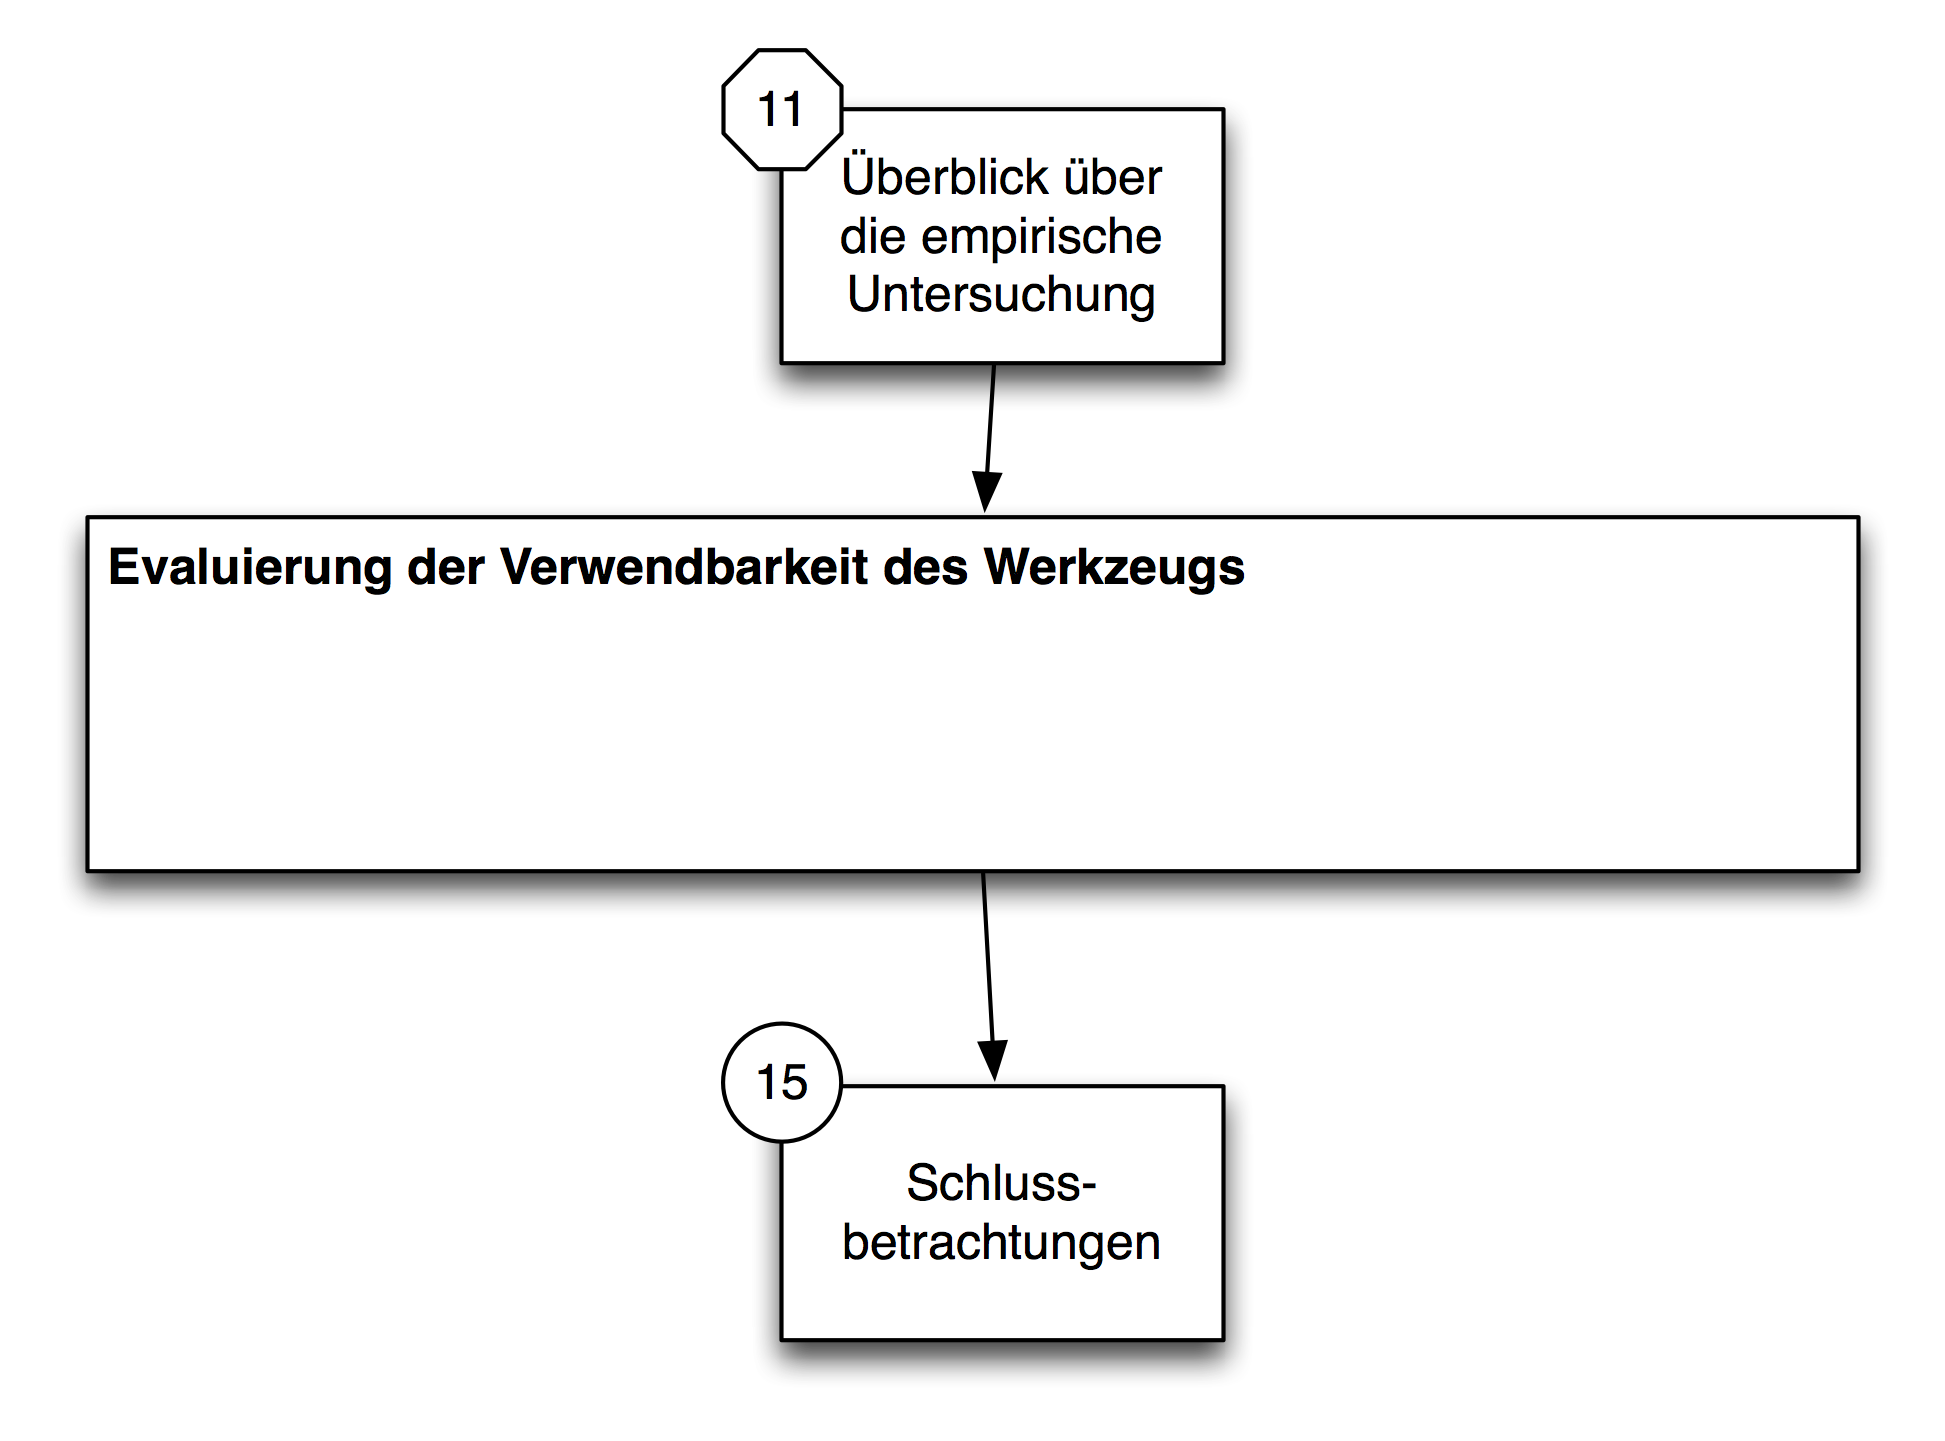
\includegraphics[scale=0.6]{img/Kontextgrafiken/k12.png}
	\caption{Kapitel „Evaluierung der Verwendbarkeit des Werkzeugs“ im Gesamtzusammenhang}
	\label{fig:img_Kontextgrafiken_k12}
\end{figure}

Die Untersuchung wird daneben auch genutzt, um explorativ die inhaltliche Verwendung des Systems zu untersuchen (d.h. wie es für seinen eigentlichen Verwendungszweck -- die Modellierung -- eingesetzt wurde) und aus diesen Beobachtungen Hypothesen abzuleiten, die in weiteren Schritten getestet werden.

\section{Hypothesen} % (fold)
\label{sec:hypothesen}

In diesem Abschnitt werden die Hypothesen angeführt und begründet, die in diesem Teil der empirischen Untersuchung geprüft werden. Die hier angegebenen Hypothesen gehen auf die Eigenschaften des Werkzeugs in der Verwendung durch die Benutzer ein. Bei der Hypothesenbildung wird auf den Verwendungszweck des Werkzeugs -- die Unterstützung der Bildung diagrammatischer Modelle -- zwar Rücksicht genommen, die Modelle selbst sind jedoch nicht Gegenstand der Betrachtung und werden erst im nächsten Kapitel behandelt. Nicht berücksichtigt wird außerdem die Verwendung des Werkzeugs zur Unterstützung von „Articulation Work“ -- diese ist Gegenstand von Kapitel \ref{cha:eval_aw}.

\subsection{Konzeptuell begründete Hypothesen} % (fold)
\label{sub:konzeptuell_begründete_hypothesen}

Die folgenden Hypothesen wurden aus der Aufgabenstellung (siehe Kapitel \ref{cha:einführung}) sowie den Anforderungen an das Werkzeug (siehe Kapitel \ref{cha:anforderungen}) abgeleitet. Neben der Formulierung der Hypothese ist jeweils die Begründung aus der Konzeption des Werkzeugs angeführt.

Der grundlegende Anspruch des Werkzeugs ist es, explizite „Articulation Work“ zu unterstützen. Wie in Teil \ref{prt:grundlagen} dieser Arbeit beschrieben, wird dies durch die Externalisierung und Abstimmung von mentalen Modellen realisiert. Ein gängiges Mittel, um mentale Modelle zu repräsentieren, ist die Verwendung von diagrammatischen Modellen, wozu Methoden zur Externalisierung -- wie Concept Mapping und Strukturlegetechniken -- genutzt werden. Das Werkzeug muss also die Repräsentation diagrammatischer Modelle unterstützen. Die Prüfung der ersten Hypothese ermöglicht damit die Beurteilung der Erfüllung der Anforderung \ref{anf:physische_abbildung_legen_beliebiger_diagrammatischer_modelle} (siehe Seite \pageref{anf:physische_abbildung_legen_beliebiger_diagrammatischer_modelle}). 

\begin{hyp}
	\label{hyp:diagmodelle}
	Das Werkzeug ermöglicht die Repräsentation diagrammatische Modelle.
\end{hyp}

„Articulation Work“ ist immer in einen kooperativen Arbeitszusammenhang eingebettet. Die Kollaboration findet dabei nicht nur im produktiven Teil der Arbeit statt, sondern hat immer auch Auswirkungen auf die „Articulation Work“. Jede Unterstützung von „Articulation Work“ muss damit auch in kooperativen Szenarien einsetzbar sein. Dies gilt auch für das hier vorgestellte Werkzeug, das die kooperative Bearbeitung einer Aufgaben (hier: der Externalisierung und Abstimmung mentaler Modelle) ermöglichen muss. Die Hypothese ist deshalb aus Anforderung \ref{anf:kollaborative_und_unmittelbare_manipulierbarkeit_des_modells} (siehe Seite \pageref{anf:kollaborative_und_unmittelbare_manipulierbarkeit_des_modells}) abgeleitet und ermöglicht die Beurteilung deren Erfüllung.

\begin{hyp}
	\label{hyp:kollaborativ}
	Das Werkzeug ermöglicht kooperatives Arbeiten an einer Aufgabe.
\end{hyp}

Die Aspekte von Arbeit, die im Rahmen von „Articulation Work“ abzustimmen sind, sind unterschiedlicher Natur. Naheliegend ist eine Abstimmung der Abläufe und Schnittstellen zwischen Personen, aber auch nicht-prozedurale Information, wie das Verständnis der Struktur und Elemente eines Arbeitszusammenhangs kann Gegenstand von „Articulation Work“ sein. Gleiches gilt für die im Rahmen der „Articulation Work“ abzustimmenden mentalen Modelle -- diese bilden die Basis für Handlungsentscheidungen, umfassen aber im Allgemeinen (in Abgrenzung zu Schemata) nicht nur handlungsleitende Information, sondern auch Kontextinformation, die die Bewertung der wahrgenommenen Situation ermöglicht. Dementsprechend muss ein Werkzeug zur Unterstützung von expliziter „Articulation Work“ und damit der Externalisierung von mentalen Modellen die Verwendung in unterschiedlichen Kontexten, d.h. für unterschiedliche zu externalisierenden Informationsstrukturen, die in mentalen Modellen abgebildet sind, ermöglichen. Die Prüfung der unten formulierten Hypothese ermöglicht die Beurteilung der Erfüllung der Anforderung \ref{anf:nicht_vorgegebene_semantik_der_modellierungselemente} (siehe Seite \pageref{anf:nicht_vorgegebene_semantik_der_modellierungselemente}).

\begin{hyp}
	\label{hyp:kontexte}
	Das Werkzeug ist gleichwertig für Modellierungsaufgaben in unterschiedlichen Kontexten einsetzbar.
\end{hyp}

Die ersten drei hier formulierten Hypothesen sind unmittelbar aus der globalen Zielsetzung abgeleitet und bilden die grundlegenden Anforderungen an das Werkzeug bei der Unterstützung von „Articulation Work“ ab. Die nun folgenden Hypothesen sind konzeptuell nicht mehr direkt auf die globale Zielsetzung ausgerichtet, sondern prüfen die Funktionalität des Werkzeugs, die den Modellbildungsprozess unterstützen soll. 

Auf Basis der Möglichkeit zur Navigation durch die Entstehungsgeschichte des Modells besteht auch die Möglichkeit, vergangene Modellzustände wiederherzustellen. Das Werkzeug unterstützt dabei die Benutzer durch die Ausgabe von schrittweisen Anweisungen, die den aktuellen Modellzustand in den wiederherzustellenden Zustand überführen. Allgemein bietet diese Funktionalität die Möglichkeit, erkannte Fehler im Modell zu korrigieren, ohne dabei bereits repräsentierte Information zu verlieren. Im kollaborativen Einsatz ermöglicht diese Funktionalität, alternative, individuelle Sichten auf den abzustimmenden Sachverhalt zu repräsentieren und bietet dabei die Möglichkeit, einen für alle Beteiligten akzeptablen Ausgangspunkt wiederherzustellen. Dies sollte die Bereitschaft zur experimentellen Veränderung von Modellen erhöhen. Die Prüfung dieser Hypothese ermöglicht in der Folge die Beurteilung der Erfüllung der Anforderung \ref{anf:ermöglichung_experimenteller_veränderungen_am_modell} (siehe Seite \pageref{anf:ermöglichung_experimenteller_veränderungen_am_modell}).

\begin{hyp}
	\label{hyp:wiederherstellung}
	Die Möglichkeit der Wiederherstellung vergangener Modellzustände fördert die Bereitschaft alternative Repräsentationen auszuprobieren.
\end{hyp}

Die letzten beiden Hypothesen dieses Abschnitts sind ausschließlich auf die Verwendung des Werkzeugs an sich ausgerichtet und stehen nicht im Kontext von „Articulation Work“ oder der Unterstützung der Externalisierung mentaler Modelle. Hypothese \ref{hyp:behinderung} steht für den in der Zielsetzung formulierten Anspruch, dass das Werkzeug in den Hintergrund treten muss und die Beschäftigung mit der eigentlichen Aufgabe nicht behindern darf. Dabei wird hier nicht auf den konkreten Anwendungsfall -- die Erstellung von Modellen -- eingegangen, sondern lediglich die allgemeine Funktionsfähigkeit und Bedienbarkeit des Werkzeugs betrachtet. Ersteres ist Gegenstand der Evaluierung der erstellten Modelle, die in Kapitel \ref{cha:eval_modell} beschrieben werden. Die Prüfung dieser Hypothese ermöglicht die Beurteilung der Erfüllung der Anforderung \ref{anf:physische_abbildung_legen_beliebiger_diagrammatischer_modelle} (siehe Seite \pageref{anf:physische_abbildung_legen_beliebiger_diagrammatischer_modelle}).

\begin{hyp}
	\label{hyp:behinderung}
	Das Werkzeug behindert die Modellbildung nicht.
\end{hyp}

Hypothese \ref{hyp:gewöhnung} geht davon aus, dass bei wiederholter Verwendung des Werkzeugs Lern- und Gewöhnungseffekte auftreten, die die Verwendung erleichtern, beschleunigen und zu weniger Fehlbedienung führen. Dies ist ein Effekt, der bei jedem Werkzeug zu erwarten ist, dessen zugrunde liegenden Konzepte den Benutzern bewusst und verständlich sind. Von dieser Voraussetzung kann durch die inhaltliche Einführung der Benutzer in die das Werkzeug prägenden und motivierenden Ideen ausgegangen werden. Damit wäre zu erwarten, dass das Werkzeug bei wiederholtem Einsatz in den späteren Anwendungen effizienter (im Sinne von „schneller“ und „Fehlbedienungen vermeidend“) verwendet wird. Die Prüfung dieser Hypothese ermöglicht die Beurteilung der Erfüllung der Anforderung \ref{anf:physische_abbildung_legen_beliebiger_diagrammatischer_modelle} (siehe Seite \pageref{anf:physische_abbildung_legen_beliebiger_diagrammatischer_modelle}).

\begin{hyp}
	\label{hyp:gewöhnung}
	Wiederholte Verwendung des Werkzeugs führt zu schnellerer Modellbildung und weniger Fehlbedienungen.
\end{hyp}

Hinsichtlich der in Kapitel \ref{cha:anforderungen} formulierten Anforderungen können die hier formulierten Hypothesen zusammenfassend wie in Tabelle \ref{hyp:eval_tui} dargestellt eingeordnet werden. Die Untersuchung der Hypothesen ist dabei der erste Schritt zur Prüfung der effektiven Unterstützung von „Articulation Work“, für die eine Verwendbarkeit des Werkzeugs für die Durchführung der vorgeschlagenen Methodik eine Voraussetzung ist.

\begin{table}[htbp]
	\centering
	\caption{Hypothesen zur Benutzbarkeit des Werkzeugs und deren Bezug zu den Anforderungen an das Werkzeug}
\begin{tabular}{|c|c|}
  \hline
   Hypothese & Anforderung \\ \hline
   \ref{hyp:diagmodelle} & \ref{anf:physische_abbildung_legen_beliebiger_diagrammatischer_modelle} \\
   \ref{hyp:kollaborativ} & \ref{anf:kollaborative_und_unmittelbare_manipulierbarkeit_des_modells} \\
   \ref{hyp:kontexte} & \ref{anf:nicht_vorgegebene_semantik_der_modellierungselemente} \\
   \ref{hyp:wiederherstellung} & \ref{anf:ermöglichung_experimenteller_veränderungen_am_modell} \\
   \ref{hyp:behinderung} & \ref{anf:physische_abbildung_legen_beliebiger_diagrammatischer_modelle} \\
   \ref{hyp:gewöhnung} & \ref{anf:physische_abbildung_legen_beliebiger_diagrammatischer_modelle} \\ \hline
\end{tabular} 
	\label{hyp:eval_tui}
\end{table}

% subsection konzeptuell_begründete_hypothesen (end)

\subsection{Explorativ gebildete Hypothesen} % (fold)
\label{sub:explorativ_gebildete_hypothesen}

Neben den aus der Aufgabenstellung abgeleiteten Hypothesen wurden einige Hypothesen auch während der Durchführung der einzelnen Evaluierungs-Blöcke gebildet. Diese Hypothesen sind spezifischer auf einzelne Aspekte des Werkzeugs ausgerichtet und decken beobachtete Auffälligkeiten und Missverständnisse in der Verwendung des Werkzeugs ab. 

Die erste in diesem Zusammenhang beobachtete Auffälligkeit betrifft die Herstellung von Verbindern zwischen einzelnen Modellelementen. Wie in Abschnitt \ref{sub:verbinden_von_modellelementen} beschrieben, existieren zwei Möglichkeiten, diese Funktion auszuführen. Einerseits können die beiden Modellelemente, die verbunden werden sollen, mit Markierungs-Tokens ausgewählt werden, woraufhin eine Verbindung hergestellt wird. Andererseits können Verbinder auch durch das Zusammenführen der zu verbindenden Blöcke (bis sich deren Breitseiten berühren) hergestellt werden. In der ersten Implementierung des Werkzeugs, die im Evaluierungsblock 1 und im ersten Teil des zweiten Blocks verwendet wurde, war lediglich die erste Variante verfügbar. Die Möglichkeit zur Herstellung von Verbindern wurde in den in diesen Blöcken durchgeführten Anwendungen kaum eingesetzt. Dies führte einerseits zur Bildung der Hypothese \ref{hyp:keine_verbinder} (siehe Abschnitt \ref{sub:m_explorativ_gebildete_hypothesen}), andererseits wurde bei ersten Auswertungen der Beobachtungen der im Verhältnis zum übrigen Modellierungs-Prozess hohe Zeit-Aufwand bei der Herstellung von Verbindern offensichtlich. Dieser Aufwand ist den Maßnahmen zur Stabilisierung der Erkennungsleistung des Werkzeugs geschuldet und kann mit dem eingesetzten Interaktionsablauf nicht reduziert werden. Aufgrund einer Anregung eines Untersuchungsteilnehmers wurde deshalb die oben beschriebene zusätzliche Möglichkeit zur Herstellung von Verbindungen implementiert. Zu untersuchen ist nun, ob diese Maßnahme die Nutzung von Verbindern bei der Modellbildung tatsächlich erhöht.

\begin{hyp}
	\label{hyp:verbinder}
	Die Einführung der alternativen Möglichkeit zur Verbindungsherstellung erhöht die Nutzung von Verbindern bei der Modellerstellung.
\end{hyp}

Die zweite hier aufgestellte Hypothese betrifft eine Auffälligkeit bei der Verwendung des Löschtokens. Das Löschtoken wird verwendet, um das Werkzeug in einen Modus zu versetzen, in dem Verbinder gelöscht werden können. Schon die konzeptuelle Einordnung des Werkzeugs in Kapitel \ref{cha:konzeptuelle_evaluierung} zeigte Potential für Missverständnisse in der Verwendung dieses Tokens (siehe z.B. die Abschnitte \ref{sec:spezifikation_des_tac_schemas_nach_shaer_et_al_} und \ref{sec:einordnung_in_die_taxonomie_von_fishkin}). Zusammengefasst liegt die aus der Theorie ableitbare Problematik darin, dass durch die äußere Form des Tokens -- einem Radiergummi -- eine Metapher für dessen Verwendung („ausradieren“ von Elementen) suggeriert wird, die in dieser Form im Werkzeug nicht umgesetzt ist, da das Token lediglich als Schalter fungiert. Erste Beobachtungen deuteten darauf hin, dass die Verwendung des Löschtokens in dessen erster Implementierung tatsächlich unverständlich oder missverständlich zu sein scheint. Das Werkzeug wurde auf Basis dieser Beobachtungen reimplementiert. Die Hypothese ist deshalb für beide Varianten zu prüfen.

\begin{hyp}
	\label{hyp:radierer}
	Das Löschtoken ermöglicht intuitives Löschen von Modellelementen.
\end{hyp}

% subsection explorativ_gebildete_hypothesen (end)
% section hypothesen (end)

\section{Untersuchungsdesign und Durchführung} % (fold)
\label{sec:untersuchungsdesign}

In diesem Abschnitt wird auf Basis der oben formulierten Hypothesen das Untersuchungsdesign abgeleitet und die Durchführung der Untersuchung beschrieben. Der erste Teil des Abschnitts beschreibt die Operationalisierung der Hypothesen und damit die Festlegung, wie diese konkret geprüft werden können. Im zweiten Teil des Abschnitts wird die Durchführung der Prüfung beschrieben. Hier erfolgt neben der Zuordnung der einzelnen Evaluierungsblöcke (siehe Abschnitt \ref{sec:globales_untersuchungsdesign}) auch die Darstellung rein beschreibender Parameter der Werkzeugverwendung, die nicht unmittelbar in die Prüfung der Hypothesen eingehen. 

\subsection{Operationalisierung} % (fold)
\label{sub:operationalisierung}

In diesem Abschnitt wird für jede Hypothese identifiziert, in welcher Form sie geprüft werden kann. Dies umfasst die Festlegung der Messpunkte sowie der jeweiligen Mess- und Auswertungsmethode (letztere bezugnehmend auf den in Abschnitt \ref{sec:eingesetzte_werkzeuge_und_verfahren} beschriebenen Verfahren). Zudem werden jene Evaluationsblöcke festgelegt, die für die jeweilige Untersuchung herangezogen wurden.

Für jede Hypothese wird also spezifiziert, anhand welcher Aspekte diese geprüft werden kann (= abhängige Variablen). Zudem wird festgelegt welche Ausgangssituation bei der Anwendung gewählt werden muss, um die Prüfung durchführen zu können (= unabhängige Variable) und welche Faktoren die Beurteilung ggf. ungewollt beeinflussen können (= Störvariablen).

\subsubsection{Repräsentation diagrammatischer Modelle} % (fold)
\label{ssub:repräsentation}

Gegenstand dieses Abschnitts ist die Prüfung der Hypothese \ref{hyp:diagmodelle}. Diese bezieht sich auf die Eignung des Werkzeugs für die Repräsentation diagrammatischer Modelle.

Voraussetzung für die Prüfung der Hypothese ist der Einsatz von Modellierungsaufgaben, die so formuliert sind, dass es grundsätzlich möglich ist, sie durch die Beschreibung in einem diagrammatischen Modell zu erfüllen. Keinen Einfluss auf die Untersuchung haben die eingesetzte Methodik sowie eventuell vorhandene Modellierungsvorkenntnisse, da die grundsätzlich Möglichkeit der Erstellung diagrammatischer Modelle unabhängig von der Art der Verwendung und von der Kompetenz der Benutzer ist. 

Geprüft wird die Hypothese hier an der Repräsentation, die mit Hilfe des Werkzeugs erstellt wurde. Ein diagrammatisches Modell zeichnet nach \citep{Larkin87} aus, dass in ihm Konzepte und deren Zusammenhänge visuell-graphisch dargestellt werden können (in Abgrenzung zu textuellen Beschreibungen). Zur Bewertung der Hypothese werden deshalb die erstellten Repräsentationen herangezogen und überprüft, ob sie den Anforderungen an ein diagrammatisches Modell -- das Vorhandensein von Konzepten und Beziehungen zwischen diesen -- erfüllen.

% subsubsection repräsentation (end)

\subsubsection{Kooperatives Arbeiten} % (fold)
\label{ssub:kollaboratives_arbeiten}

Gegenstand dieses Abschnitts ist die Prüfung der Hypothese \ref{hyp:kollaborativ}. Dabei wird überprüft, ob das Werkzeug kooperatives Arbeiten an einer Modellierungsaufgabe erlaubt.

Dazu muss eine Modellierungsaufgabe gewählt werden, in der die kooperatives Erstellung des Modells vorgesehen ist. Etwaige Modellierungsvorkenntnisse haben keinen Einfluss auf die Beurteilung der hier betrachteten Hypothese.

Zur Beurteilung eignen sich in diesem Fall die Zeitverteilung der Beteiligung der einzelnen Benutzer am Modellierungsvorgang, das Verhalten der Benutzer bei simultaner Manipulation eines Modells auf der Modellierungsoberfläche sowie der subjektive Eindruck der Benutzer über deren Kooperation untereinander. Der erstgenannte Aspekt kann quantitativ gemessen werden, wobei eine tendenziell zeitlich gleichverteilte Einbindung der Beteiligten in die Modellbildung für die Annahme der Hypothese spricht. Zusätzlich kann mittels dem zweiten und dritten Aspekt qualitativ beurteilt werden, ob und wie eine kooperative Manipulation des Modells durch mehrere Benutzer gleichzeitig möglich ist.

% subsubsection kollaboratives_arbeiten (end)

\subsubsection{Einsetzbarkeit in unterschiedlichen Kontexten} % (fold)
\label{ssub:einsetzbarkeit_in_unterschiedlichen_kontexten}

Gegenstand dieses Abschnitts ist die Operationalisierung der Hypothese \ref{hyp:kontexte}. Diese Hypothese zielt dabei auf die Eignung des Werkzeugs zur Modellbildung in unterschiedlichen Kontexten, d.h. für unterschiedliche Modellierungsaufgaben ab. 

Zur Beurteilung dieser Hypothese muss die Modellierungsaufgabe entsprechend den unterschiedlichen Einsatzkontexten variiert werden. Etwaige Modellierungsvorkenntnisse können die individuelle Beurteilung insofern beeinflussen, als dass sie Werkzeuge für eine bestimmte Aufgabe als besser oder schlechter geeignet erscheinen lassen.

Zur Prüfung der Hypothese bieten sich in diesem Fall die Wahrnehmung der Eignung durch die Benutzer, die qualitativ beurteilt wird und die Korrelation der Größe der erstellten Modelle mit der benötigten Modellierungsdauer an. Korrelliert die Modellgröße positiv mit der Modellierungsdauer, so ist der Zeitanteil, der zu Beschäftigung mit dem Werkzeug selbst (und nicht mit der Modellierungsaufgabe) tendenziell stabil. Daraus kann abgeleitet werden, dass das Werkzeug die verglichenen Modellierungsaufgaben gleich gut (oder schlecht) unterstützt.

% subsubsection einsetzbarkeit_in_unterschiedlichen_kontexten (end)

\subsubsection{Wiederherstellung vergangener Modellzustände} % (fold)
\label{ssub:wiederherstellung_vergangener_modellzustände}

Gegenstand dieses Abschnitts ist die Operationalisierung der Hypothese \ref{hyp:wiederherstellung}. Gegenstand der Überprüfung ist die Verwendung der Wiederherstellungsfunktionalität zum Zwecke der versuchsweisen Veränderung des Modells.

Zur Prüfung dieser Hypothese muss die Modellierungsaufgabe so gestaltet sein, dass sinnvoll unterschiedliche Repräsentationen gebildet werden können. Modellierungsvorkenntnisse haben keine Auswirkungen auf diese Untersuchung.

Zur Beurteilung dieser Hypothese wird die Anzahl der Verwendungen der Wiederherstellungsfunktionalität zur Korrektur inhaltlich verworfener Repräsentationen herangezogen. Höhere Werte deuten hier tendenziell auf eine Annahme der Hypothese hin. Zusätzlich können qualitative Aussagen zur Nutzung dieser Funktionalität und deren wahrgenommenen Nutzen zur Beurteilung verwendet werden. 

% subsubsection wiederherstellung_vergangener_modellzustände (end)

\subsubsection{Nicht-Behinderung} % (fold)
\label{ssub:nicht_behinderung}

Gegenstand dieses Abschnitts ist die Operationalisierung der Hypothese \ref{hyp:behinderung}. Dabei wird überprüft, ob bei der Verwendung des Werkzeugs dieses in den Aufmerksamkeitsfokus der Benutzer tritt oder sich diese auf die eigentliche Modellierungsaufgabe konzentrieren können. 

Die Modellierungsaufgabe hat keinen Einfluss auf die Überprüfung dieser Hypothese, lediglich etwaig vorhandene Modellierungsvorkenntnisse können die Beurteilung beeinträchtigen, da sie Einfluss auf die erwartete Funktionalität des Werkzeugs haben kann.

Zur Beurteilung, ob bzw. inwieweit das Werkzeug die Modellbildung behindert, werden sowohl quantitativ als auch qualitativ beurteilbare Metriken herangezogen. Die Anzahl von Fehlfunktionen des Werkzeugs bzw. das Auftreten von Systemabstürzen kann als Indikator für eine behindernde Wirkung des Werkzeugs herangezogen werden. Das Auftreten von Missverständnissen und daraus resultierende Fehlbedienungen können ebenfalls eine Behinderung des Modellierungsvorgangs interpretiert werden. Zudem werden Aussagen der Benutzer hinsichtlich hinderlicher Faktoren bei der Werkzeugbenutzung als Maß für die wahrgenommene Behinderung durch das Werkzeug herangezogen.

% subsubsection nicht_behinderung (end)

\subsubsection{Gewöhnung an das Werkzeug} % (fold)
\label{ssub:gewöhnung_an_das_werkzeug}

Gegenstand dieses Abschnitts ist die Operationalisierung der Hypothese \ref{hyp:gewöhnung}. Dabei wird überprüft, ob wiederholte Benutzung des Werkzeugs Auswirkung auf die Qualität der Interaktion hat. Eine Erhöhung der Qualität äußert sich in schnellerer Modellbildung und weniger Fehlbedienung.

Bei der Prüfung der Hypothese muss eine etwaige veränderte Funktionalität des Werkzeugs zwischen den verglichenen Evaluierungsblöcken berücksichtigt werden, die die Interaktion einerseits erleichtern kann, andererseits aber auch zu Fehlbedienung aufgrund von unbekannten Interaktionsmustern führen kann. Auch unterschiedliche Modellierungsaufgaben, die ein Individuum in den aufeinander folgenden Anwendungen bearbeitet, können die Beurteilung erschweren, weil potentiell andere (noch unbekannte) Funktionen des Werkzeugs zum Einsatz kommen können.

Zur Beurteilung der Qualität der Interaktion sind einerseits die Anzahl der Fehlbedienungen des Werkzeugs pro Zeiteinheit und andererseits die Arbeitsdauer am Werkzeug\footnote{Die Arbeitsdauer am Werkzeug ist im Gegensatz zur gesamten Modellierungsdauer um jenen Zeitanteil reduziert, in dem die Teilnehmer interagieren, ohne am Werkzeug zu arbeiten.} in Abhängigkeit der Modellgröße heranzuziehen. Die Normierung der Arbeitsdauer ist notwendig, um vergleichbare Werte für unterschiedliche Werkzeug-Anwendungen zu erhalten. Sinken beide Werte zwischen zwei Evaluierungsblöcken, die auf der gleichen Stichprobe aufbauen, signifikant, so kann die Hypothese bestätigt werden. Um eine Vergleichbarkeit zwischen den Anwendungen herzustellen, ist es sinnvoll, in beiden Blöcken eine identische Modellierungsaufgabe zu stellen und die Funktionalität des Werkzeugs nicht zu verändern. Identische Modellierungsaufgaben können durch die wiederholte inhaltliche Beschäftigung mit der Aufgabe zu schnellerer Arbeit bzw. zu kompakteren Modellen führen. Dies kann wiederum durch die Berücksichtigung der reinen Arbeitszeit am Werkzeug sowie der Normierung derselben in Abhängigkeit der Modellgröße kompensiert werden.

% subsubsection gewöhnung_an_das_werkzeug (end)

\subsubsection{Herstellung von Verbindern} % (fold)
\label{ssub:herstellung_von_verbindern}

Gegenstand dieses Abschnitts ist die Operationalisierung der Hypothese \ref{hyp:verbinder}. Mit Hilfe dieser Hypothese soll überprüft werden, ob die Einführung der alternativen Möglichkeit zur Herstellung von Verbindern deren Verwendung signifikant gesteigert hat.

Bei der Messung muss der Einfluss der Modellierungsaufgabe (da sie die Anzahl der benötigten Verbinder beeinflussen kann) und eventuell vorhandene Modellierungsvorkenntnisse (da diese Einfluss auf die Struktur des Modells haben können) berücksichtigt werden. Um den Einfluss dieser Aspekte zu reduzieren, wird die Beurteilung in zwei Evaluierungsblöcken vorgenommen, in denen die gleiche Stichprobe mit der gleichen Aufgabenstellung das Werkzeug mit der gleichen Methodik verwendet. Lediglich die Funktionalität des Werkzeugs wurde zwischen den beiden Anwendungen um den alternativen Weg zur Herstellung von Verbindern erweitert.  

Zur Beurteilung des Ausmaßes der Verwendung von Verbindern kann die Connectedness des Modells herangezogen werden. Die Connectedness ist das Verhältnis zwischen der Anzahl der im Modell verwendeten Verbinder und der Anzahl der verwendeten Knoten (Modellierungselemente). Hier ist zu prüfen, ob die Connectedness in jenem Evaluierungs-Block, in dem der alternative Weg zur Herstellung von Verbindungen verfügbar war, signifikant höher ist als in jenem Block, in dem sie nicht verfügbar war.

% subsubsection herstellung_von_verbindern (end)

\subsubsection{Verwendung des Löschtokens} % (fold)
\label{ssub:löschtoken}

Gegenstand dieses Abschnitts ist die Operationalisierung der Hypothese \ref{hyp:radierer}. Dabei wird überprüft, ob das Löschtoken intuitiv korrekt verwendet wird oder ob es zu Fehlinterpretationen kommt.

Die Verwendbarkeit des Löschtokens ist unabhängig von der Modellierungsaufgabe, der angewandten Methodik und auch von eventuell vorhandenen Modellierungsvorkenntnissen. Hinsichtlich des Anwendungskontextes des Werkzeugs sind also keine Voraussetzungen zu beachten.

Zur Beurteilung der intuitiven Verwendbarkeit werden quantitative und qualitative Merkmale der Werkzeugverwendung herangezogen. Quantitativ beurteilbar ist der Anteil der Fehlbedienungen des Löschtokens in Bezug auf alle Anwendungen des Werkzeugs, in denen es grundsätzlich verwendet wurde. Qualitativ wird die Art des Missverständnisses, das zu den jeweiligen Fehlbedienungen führt, beurteilt.

Zur Messung der quantitativen Variablen wird für jede Anwendung die Anzahl der Fehlbedienungen erhoben, die durch das Löschtoken verursacht wurden. Diese Anzahl wird ins Verhältnis zur Gesamtzahl der Anwendungen des Löschtokens bzw. zur gesamten Anzahl der Löschvorgänge gesetzt. Zu letzterer zählen neben den Anwendungen des Löschtokens auch Fehlerkorrekturen durch Verwendung der Wiederherstellungsfunkion. Da die zweite Möglichkeit sowohl zeit- als auch ressourcenaufwändiger zu verwenden ist als der Einsatz der Löschtokens deutet ein hoher Anteil der Verwendung dieser Funktion auf funktionale Probleme oder Verständnisprobleme der eigentlichen Löschfunktion mittels dem Löschtoken hin.  

Qualitativ werden Modellierungssituationen betrachtet, in denen das Löschtoken zum Einsatz kommt. Auf Basis von Transkripten der Interaktion zwischen den Benutzern und dem Werkzeug, bei denen es zu Fehlbedierungen kam, werden die aufgetretenen Missverständnisse explizit identifziert.

% subsubsection löschtoken (end)

% subsection operationalisierung (end)

\subsection{Durchführung} % (fold)
\label{sub:durchführung}

In diesem Abschnitt werden die für diesen Evaluierungs-Teil relevanten deskriptiven Parameter der berücksichtigten Anwendungs-Blöcke angeführt.
Als Grundlage der Überprüfung der Hypothesen werden hier die Evaluierungsblöcke 1 bis 5 verwendet. Dabei wurden für die quantitativ zu prüfenden Variablen die Blöcke 2, 3 und 5 herangezogen, da in diesen die größten Stichproben zur Verfügung standen. In die qualitative Auswertung der Ergebnisse wurden hingegen alle Blöcke (1-5) mit einbezogen.

\subsubsection{Stichprobe} % (fold)

Für die Untersuchung der Hypothesen in diesem Kapitel wurden die Evaluierungsblöcke 1 bis 5 herangezogen. Die Stichprobe setzt sich wie in Tabelle \ref{tab:stichprobe_tui} beschrieben zusammen.

\begin{table}[htbp]
	\centering
	\caption{Stichproben der Evaluierung zur Werkzeugverwendung}

		\begin{tabular}{| c | l || c | c |}
		\hline
			& Evaluierungsblock & $n_{Anwendungen}$ & $n_{Teilnehmende}$ \\ \hline
			1 & technische Evaluierung		  &  9 & 18 \\
			2a & Aushandlung 1 (1. Durchgang)  &  9 & 19 \\
			2b & Aushandlung 1 (2. Durchgang)  &  9 & 18 \\
			3 & Concept Mapping 1			  & 18 & 54 \\
			4 & Aushandlung 2				  & 10 & 13 \\
			5 & Concept Mapping 2 (Tisch)     & 11 & 24 \\  \hline
			& Gesamt						  & 66 & 146 \\ \hline
	\end{tabular}
	\label{tab:stichprobe_tui}
\end{table}

\subsubsection{Dauer der Werkzeugverwendung} % (fold)

Die Dauer der Werkzeug-Verwendung wurde in allen Evaluierungsblöcken erhoben. Die Bearbeitungszeit ist wie in Tabelle \ref{tab:dauer_werkzeugverwendung} dargestellt verteilt (siehe auch Abbildung \ref{fig:img_Evaluierung_usageTimeOverview}\footnote{In allen Boxplots gilt folgende Notation: 
\begin{itemize}
	\item dicke Linie bzw. Box: Bereich zwischen 25\%- und 75\%-Quantil
	\item breite Linie quer zur Hauptachse: Median (in horizontalen Boxen) bzw. Mittelwert (in vertikalen Boxen)
	\item linke bzw. untere schmale Linie: Bereich zwischen 2,5\%- und 25\%-Quantil
	\item rechte bzw. obere schmale Linie: Bereich zwischen 75\%- und 97,5\%-Quantil
	\item Kreuze bzw. Kreise: Ausreißer (außerhalb 2,5\%- und 97,5\%-Quantil)
\end{itemize}
}):

\begin{table}[htbp]
	\centering
	\caption{Dauer der Werkzeugverwendung}
		\begin{tabular}{| l || c | c | c | c |}
		\hline
			Evaluierungsblock & $t_{min}$ & $\overline{t}$ & $sd(t)$ & $t_{max}$ \\ \hline
			technische Evaluierung		  &  5:00 & 07:49 &  2:13 & 12:00 \\
			Aushandlung 1 (1. Durchgang)  & 11:54 & 20:53 &  4:18 & 27:30 \\
			Aushandlung 1 (2. Durchgang)  &  2:05 &  9:49 &  5:20 & 19:29 \\
			Concept Mapping 1			  & 14:01 & 32:32 & 10:07 & 45:00 \\
			Aushandlung 2				  & 15:09 & 36:25 & 13:29 & 60:12 \\
			Concept Mapping 2 (Tisch)     & 21:08 & 34:18 &  9:11 & 54:00 \\  \hline
	\end{tabular} \\
	\footnotesize Format der Zeitangaben: mm:ss
	\label{tab:dauer_werkzeugverwendung}
\end{table}


\begin{figure}[htbp]
	\centering
		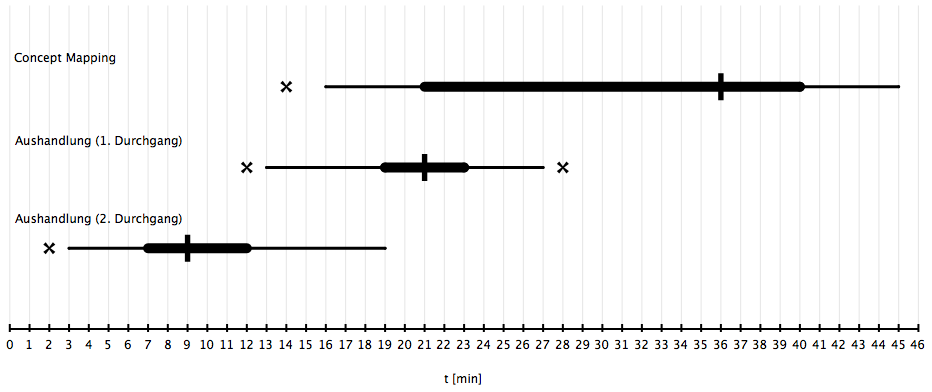
\includegraphics[width=15cm]{img/Evaluierung/usageTimeOverview.png}
	\caption{Dauer der Werkzeugverwendung -- Überblick}
	\label{fig:img_Evaluierung_usageTimeOverview}
\end{figure}

Die erhobene Dauer der Werkzeug-Verwendung teilt sich ein einen Anteil, an dem tatsächlich mit dem Werkzeug interagiert wird und einen Anteil, der anderen Tätigkeiten (wie inhaltlicher Diskussion, Bedeutungsaushandlung, \ldots) gewidmet ist. Diese beiden Anteile sind in den Evaluierungsblöcken 2 und 3 wie in den Abbildungen \ref{fig:img_Evaluierung_usageTimeConceptMapping} und \ref{fig:img_Evaluierung_usageTimeNegotiation} dargestellt verteilt. Diese beiden Evaluierungblöcke wurden prototypisch als Repräsentanten unterschiedlicher Aufgabentypen („ablauforientierte Strukturen“ in Evaluierungblock 2 und „konzeptuelle Strukturen“ in Evaluierungsblock 3) ausgewählt, die auch in den übrigen Evaluierungsblöcken zu identifizieren sind (in Evaluierungsblock 4 traten beide Typen auf, Evaluierungblock 5 erfordert die Abbildung konzeptueller Strukturen).

\begin{figure}[htbp]
	\centering
		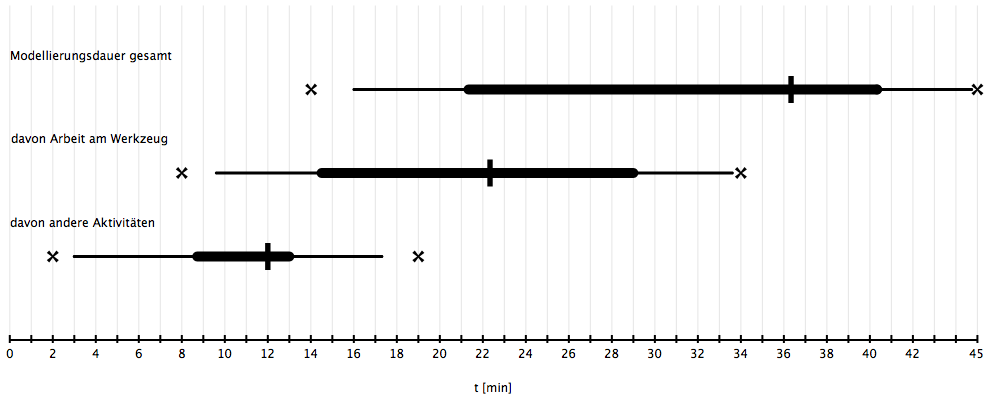
\includegraphics[width=15cm]{img/Evaluierung/usageTimeConceptMapping.png}
	\caption{Dauer der Werkzeugverwendung -- Evaluierungblock 3}
	\label{fig:img_Evaluierung_usageTimeConceptMapping}
\end{figure}

\begin{figure}[htbp]
	\centering
		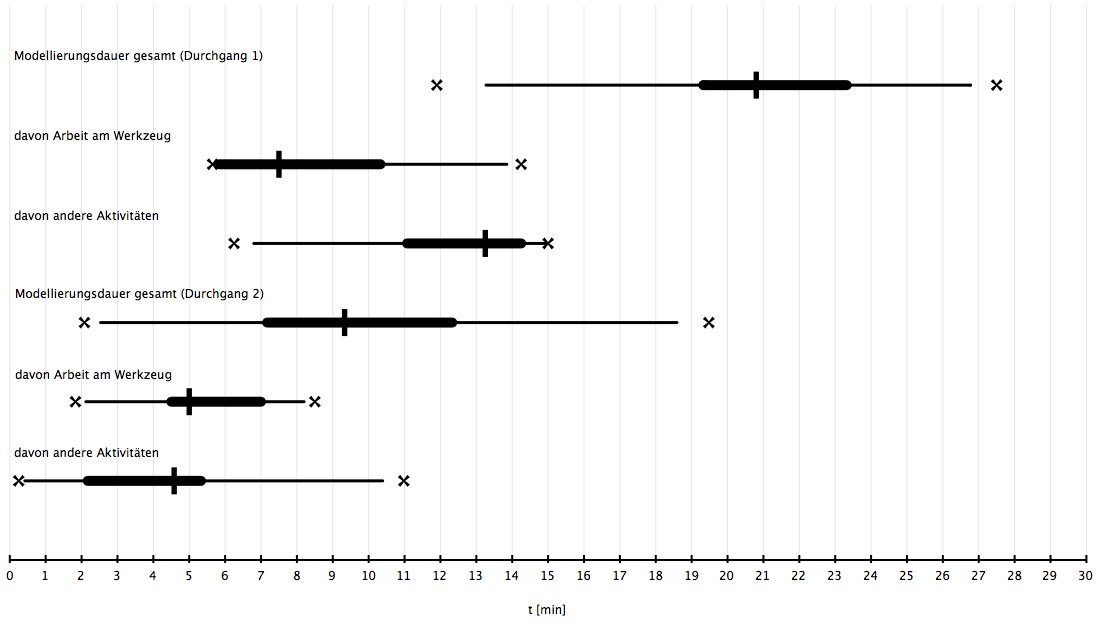
\includegraphics[width=15cm]{img/Evaluierung/usageTimeNegotiation.png}
	\caption{Dauer der Werkzeugverwendung -- Evaluierungblock 2}
	\label{fig:img_Evaluierung_usageTimeNegotiation}
\end{figure}

% subsection durchführung (end)
% section untersuchungsdesign (end)

\section{Ergebnisse} % (fold)
\label{sec:ergebnisse}

In diesem Abschnitt werden die Ergebnisse der Untersuchung gegliedert nach den oben formulierten Hypothesen dargestellt. Zu jeder Hypothese wird die Auswertung der empirischen Daten dargestellt, die Bedeutung der empirischen Belege für die Prüfung der jeweiligen Hypothese diskutiert und letztendlich das Ergebnis zusammenfassend dargestellt.  

\subsection{Repräsentation diagrammatischer Modelle} % (fold)
\label{sub:repräsentation_diagrammatischer_modelle}

Gegenstand der hier beschriebenen Untersuchung ist Hypothese \ref{hyp:diagmodelle} („Das Werkzeug ermöglicht die Repräsentation diagrammatischer Modelle.“). Als Grundlage dieser Untersuchung dienen die Ergebnisse aller Evaluierungsblöcke, da die Aufgaben in allen Fällen auf die Erstellung einer Repräsentation in Form eines diagrammatischen Modells gefordert war.

Ausgewertet wird hier, ob die Ergebnisse der Modellierung jeweils als diagrammatisches Modell zu klassifizieren sind. Ein diagrammatisches Modell zeichnet sich nach \citep{Larkin87} dadurch aus, dass in ihm Konzepte und deren Zusammenhänge visuell-graphisch dargestellt werden. Eine Darstellung von Beziehungen kann durch die explizite Darstellung von Verbindungen zwischen Konzepten oder durch andere graphische Mittel wie Gruppierung von Konzepten in räumlicher Nähe erfolgen. Um eine eindeutige Auswertbarkeit gewährleisten zu können, wird hier auf die explizite Darstellung von Verbindungen eingeschränkt. 

\subsubsection{Auswertung} % (fold)

In allen vorliegenden Modellen wurden Konzepte als Grundelemente des diagrammatischen Modells verwendet. Das Kriterium zur Klassifizierung als diagrammatisches Modell ist im Folgenden also das Vorhandensein von Verbindungen. Bei der Auswertung ergab sich die in Tabelle \ref{tab:modelle_mit_verbindern} dargestellte Verteilung.

\begin{table}[htbp]
	\centering
	\caption{Anzahl der Modelle mit Verbindern}

\begin{tabular}{| c || c | c |}
  \hline
   Block & Modelle gesamt & Modelle mit Verbindern \\ \hline
   1 & 9 & 0 \\ 
   2 & 18 & 9 \\ 
   3 & 18 & 17 \\ 
   4 & 10 & 10 \\ 
   5 & 11 & 11 \\ \hline
   Gesamt & 66 & 47 \\ \hline
\end{tabular}
	\label{tab:modelle_mit_verbindern}
\end{table}

Insgesamt sind in 66 Modellen, die als Ergebnis vorliegen, 47 Modelle zu identifizieren, in denen explizit Verbindungen zur Darstellung von Beziehungen zwischen Konzepten verwendet werden ($71,2\%$). Eine implizite Darstellung von Beziehungen ist jedoch in allen vorliegenden Modellen zu erkennen. Nicht explizit durch Verbindungen abgebildete Beziehungen werden in allen Fällen durch die räumliche Konfiguration der Konzepte zueinander dargestellt.

\subsubsection{Diskussion} % (fold)

Legt man das Kriterium des Vorhandenseins von Verbindungen zwischen Konzepten an, so sind $71,2\%$ der betrachteten Modelle als diagrammatische Modelle zu klassifizieren. Dies erscheint vordergründig ein geringer Wert zu sein, die gegen die allgemeine Gültigkeit der Hypothese sprechen würde. Allerdings sind in allen Modellen implizite Verbindungen zwischen Konzepten eindeutig zu identifizieren. Außerdem ist zu erkennen, dass der Anteil an diagramatischen Modellen über die Evaluierungsblöcke (und damit die Weiterentwicklung des Werkzeugs über die Zeit) hinweg stetig ansteigt, bis er in den letzten beiden Blöcken jeweils $100\%$ erreicht. Dies ist durch technische Fehlfunktionen zu erklären, die es in ersten Evaluierungsblöcken schwer bzw. teilweise unmöglich machten, intentional explizite Verbindungen zu erstellen. Unter Anbetracht dieser Erkenntnisse erscheint die Annahme der Hypothese \ref{hyp:diagmodelle} als gerechtfertigt.

Die Abbildung von Verbindungen durch räumliche Konfiguration ist Gegenstand der Prüfung von Hypothese \ref{hyp:keine_verbinder} in Kapitel \ref{cha:eval_modell} und wird dort einer näheren Betrachtung unterzogen.

\subsubsection{Ergebnis} % (fold)

\textbf{Hypothese \ref{hyp:diagmodelle} kann auf Basis der Untersuchung bestätigt werden.} Die Abbildung von Konzepten und Beziehungen zwischen diesen wurde in allen vorliegenden Modellen erfolgreich umgesetzt, wenngleich die Modellierung von expliziten Verbindungen in den ersten beiden Evaluierungsblöcken aufgrund von technischen Unzulänglichkeiten nicht durchgeführt wurde.

% subsection repräsentation_diagrammatischer_modelle (end)

\subsection{Kooperatives Arbeiten} % (fold)
\label{sub:kollaboratives_arbeiten}

Gegenstand der hier beschriebenen Untersuchung ist Hypothese \ref{hyp:kollaborativ} („Das Werkzeug ermöglicht kooperatives Arbeiten an einer Aufgabe.“). Zur Untersuchung der quantitativ beurteilbaren Aspekte wurden die Werkzeuganwendungen aus den Evaluierungsblöcken 2 ($n=18$), 3 ($n=18$) und 5 ($n=11$) herangezogen, wobei in Block 2 und 5 in Gruppen zu zwei Personen modelliert wurde (in insgesamt drei Fällen drei Personen), in Block 3 in Gruppen zu drei Personen (in drei Fällen nur zwei Personen). Zusätzlich wurden zur qualitative Beurteilung Daten aus den Blöcken 4 und 5 verwendet.

In den Evaluierungsblöcken 4 und 5 wurde hinsichtlich der subjektiven Wahrnehmung der Kooperation eine Befragung der Teilnehmer mittels eines Fragebogens durchgeführt (diese umfasste auch weitere Aspekte, die in späteren Abschnitten besprochen werden). Die Fragestellungen zur Kooperation wurde in geschlossenen Items codiert, die auf einer 7-teiligen Likert-Skala zu beantworten waren (zu den konkreten Fragebogen-Items siehe weiter unten sowie Anhang \ref{cha:daten_der_empirischen_untersuchung}). Zusätzlich wurden offene Fragen hinsichtlich der Nützlichkeit der Werkzeugs eingesetzt, die an dieser Stelle ebenfalls hinsichtlich Aussagen zur Kooperation zwischen den Teilnehmern ausgewertet werden. 

Zur Auswertung dieser Hypothese wurden außerdem die Interaktionsanalyse berücksichtigt, die in den Evaluierungsblöcken 2 bis 5 durchgeführt wurden. Herangezogen wurden dabei jene Szenen, in denen die Kooperation zwischen den jeweiligen Teilnehmern im Vordergrund stand.

\subsubsection{Auswertung} % (fold)

Grundlage des ersten Teils der Auswertung ist die Verteilung der Modellierungsdauer zwischen den Teilnehmern. Um die unterschiedliche Gesamt-Modellierungsdauer in den einzelnen Anwendungen zu kompensieren, wurden die Berechnungen auf Basis der prozentuellen Zeitanteile der einzelnen Teilnehmer durchgeführt. Die einzelnen Datensätze wurden so sortiert, dass die anteilsmäßige Modellierungsdauer von Teilnehmer A bis Teilnehmer C (bzw. B) abnimmt. In den einzelnen Evaluierungsblöcken ergeben sich die in Abbildung \ref{fig:img_Evaluierung_timeDist} dargestellten Verteilungen.

\begin{figure}[htbp]
	\centering
		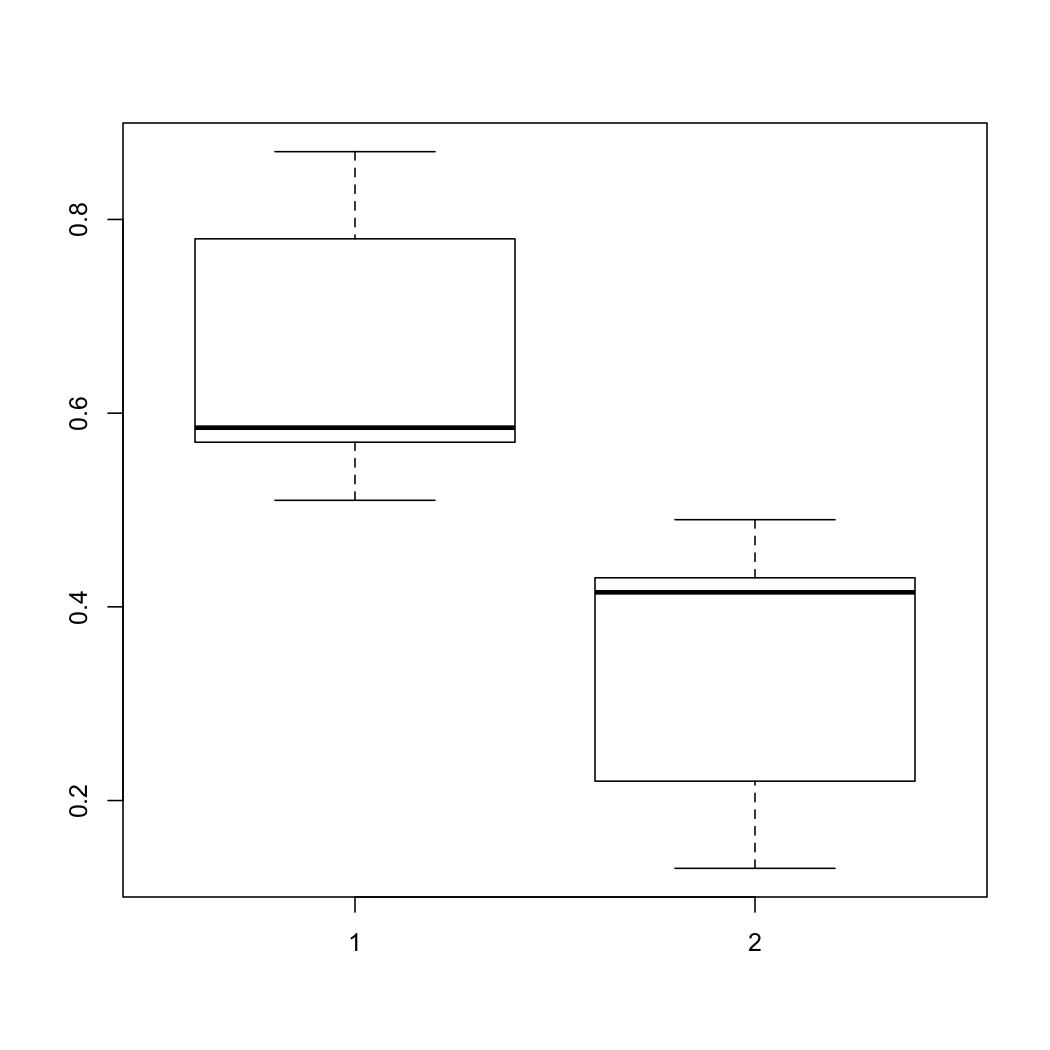
\includegraphics[height=2.5in]{img/Evaluierung/timeDist2TN.png}
		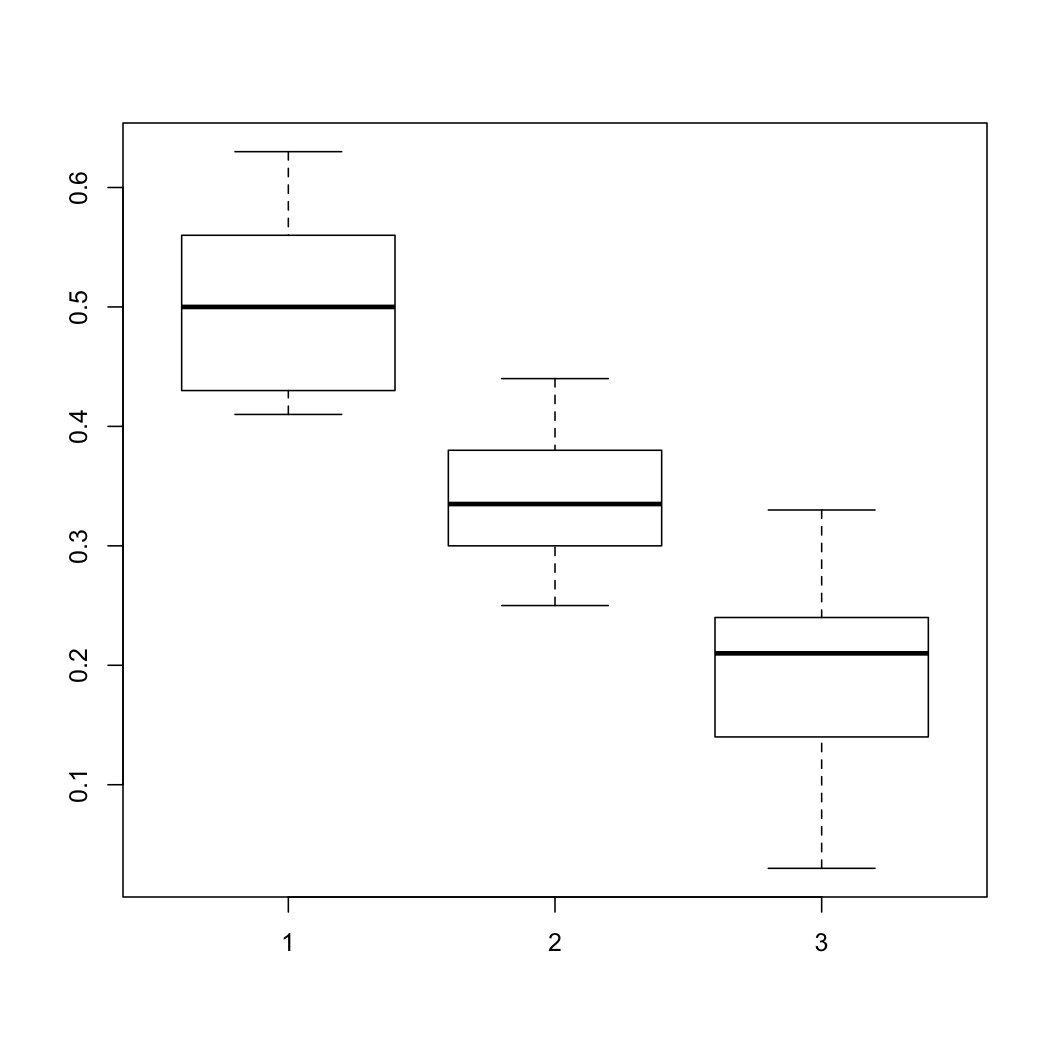
\includegraphics[height=2.5in]{img/Evaluierung/timeDist3TN.png}
	\caption[Zeitverteilung zwischen den Teilnehmern]{Zeitverteilung zwischen den Teilnehmern (1 .. TN A, 2 .. TN B, 3 .. TN C)}
	\label{fig:img_Evaluierung_timeDist}
\end{figure}

Zu prüfen ist hier, ob die Zeit-Anteile der einzelnen Teilnehmer signifikant unterschiedlich sind. Dazu wird für über die Evaluierungsblöcke hinweg die Signifikanz zwischen den Verteilungen der einzelnen Teilnehmerklassen berechnet (eine Teilnehmerklasse setzt sich aus all jenen Teilnehmern zusammen, die am längsten, am zweitlängsten bzw. am drittlängsten aktiv waren).

Für jene Anwendungen, an denen 2 Teilnehmer beteiligt waren ($n=28$) lag der durchschnittliche Zeitanteil an der Modellierung für Teilnehmer A bei $65.4\%$ ($SD=12.2\%$), jener von Teilnehmer B lag bei $34.6\%$ ($SD=12.2\%$). Die Zeitanteile unterscheiden sich damit signifikant voneinander, es ist keine Gleichverteilung der Modellierungszeiten gegeben (zweiseitiger Wilcoxon-Test für gepaarte Stichproben: $V=351, p<0.005$\footnote{Der t-Test kann nicht angewandt werden, da beide Stichproben nicht normalverteilt sind (Shaprio-Wilk-Test: $W_{TN A}=0.826, p_{TN A}<0.005$, $W_{TN B}=0.820, p_{TN B}<0.005$).}).

Für jene Anwendungen, an denen 3 Teilnehmer beteiligt waren ($n=19$) lag der durchschnittliche Zeitanteil an der Modellierung für Teilnehmer A bei $49.3\%$ ($SD=7.2\%$), jener von Teilnehmer B lag bei $33.1\%$ ($SD=5.9\%$) und jener von Teilnehmer C bei $17.6\%$ ($SD=8.2\%$). Die Zeitanteile unterscheiden sich damit signifikant voneinander, es ist keine Gleichverteilung der Modellierungszeiten gegeben (Kruskal-Wallis-Test für mehr als zwei Stichproben: $\chi^{2}=43.65, df=2, p<0.005$\footnote{Der t-Test könnte grundsätzlich für die paarweise Testung ebenfalls angewandt werden, da für alle drei Stichproben nicht davon ausgegangen werden kann, dass sie nicht normalverteilt sind (Shaprio-Wilk-Test: $W_{TN A}=0.9075, p_{TN A}=0.078$, $W_{TN B}=0.9523, p_{TN B}=0.463$, $W_{TN C}=0.9523, p_{TN C}=0.463$) und auch der Test der Varianzen eine Gleichheit derselben vermuten lässt (paarweiser F-Test: $F_{AB}=1.47, p_{AB}=0.434$, $F_{AC}=0.778, p_{AC}=0.610$, $F_{BC}=0.528, p_{BC}=0.199$). Die errechneten paarweisen Werte für t weisen ebenfalls jeweils einen signifikanten Unterschied der Zeitanteile hin ($t_{AB}=7.32, t_{AC}=12.30, t_{BC}=6.49$, $p$ jeweils $<0.005$)}).

In den Evaluierungsblöcken 4 und 5 wurden die Teilnehmer quantitativ und qualitativ nach dem Einfluss des Werkzeugs auf die Kooperation befragt. In der quantitativen Auswertung wurden 4 Items (Abschnitt „Kollaboration beim Modellieren“ in Block 4 -- siehe Anhang \ref{sub:fb_eval4} -- und Abschnitt „Kollaboratives Modellieren“ in Block 5 -- siehe Anhang \ref{sub:fb_eval5}) betrachtet. Die Items lauten im Einzelnen:

\begin{enumerate}
	\item Die Zusammenarbeit als Team empfand ich als angenehm.
	\item Die Zusammenarbeit als Team fand ich als nützlich.
	\item Ich konnte meine persönliche Meinung und Ideen ausreichend einbringen.
	\item Das Werkzeug hat die Zusammenarbeit als Team erleichtert.
\end{enumerate}

Insgesamt wurden $n=37$ Teilnehmer befragt. Die Ergebnisse sind in Tabelle \ref{tab:kooperative_modellierung} und Abbildung \ref{fig:img_Evaluierung_kollaboration} zusammengefasst dargestellt. Neben dem Mittelwert und der Standardabweichung wurde für jedes Item auch geprüft, ob die Einschätzung als signifikant positiv zu bezeichnen ist. Dazu wurde ein einseitiger Wilcoxon-Test für die Stichprobe gegenüber dem Skalenmittelwert 4 durchgeführt {Der Wilcoxon-Test muss angewandt werden, da die Stichprobe in allen vier Fällen nicht normalverteilt ist (Shapiro-Wilk-Test: $W_{1}=0.723, p{1}<0.005$, $W_{2}=0.494, p{2}<0.005$, $W_{3}=0.751, p{3}<0.005$, $W_{4}=0.853, p{4}<0.005$)}).

\begin{table}[htbp]
	\centering
	\caption{Befragung Kooperative Modellierung -- Itemauswertung}

\begin{tabular}{| c || c | c || c | c |}
  \hline
   Item & M & SD & $V_{M<4}$ & $p_{M<4}$ \\ \hline
   1 & $1.51$ & $0.61$ & 0 & <0.005 \\ 
   2 & $1.62$ & $1.04$ & 27.5 & <0.005 \\ 
   3 & $1.62$ & $0.79$ & 0 & <0.005 \\ 
   4 & $2.16$ & $1.14$ & 4 & <0.005 \\ \hline
\end{tabular}
	\label{tab:kooperative_modellierung}
\end{table}

\begin{figure}[htbp]
	\centering
		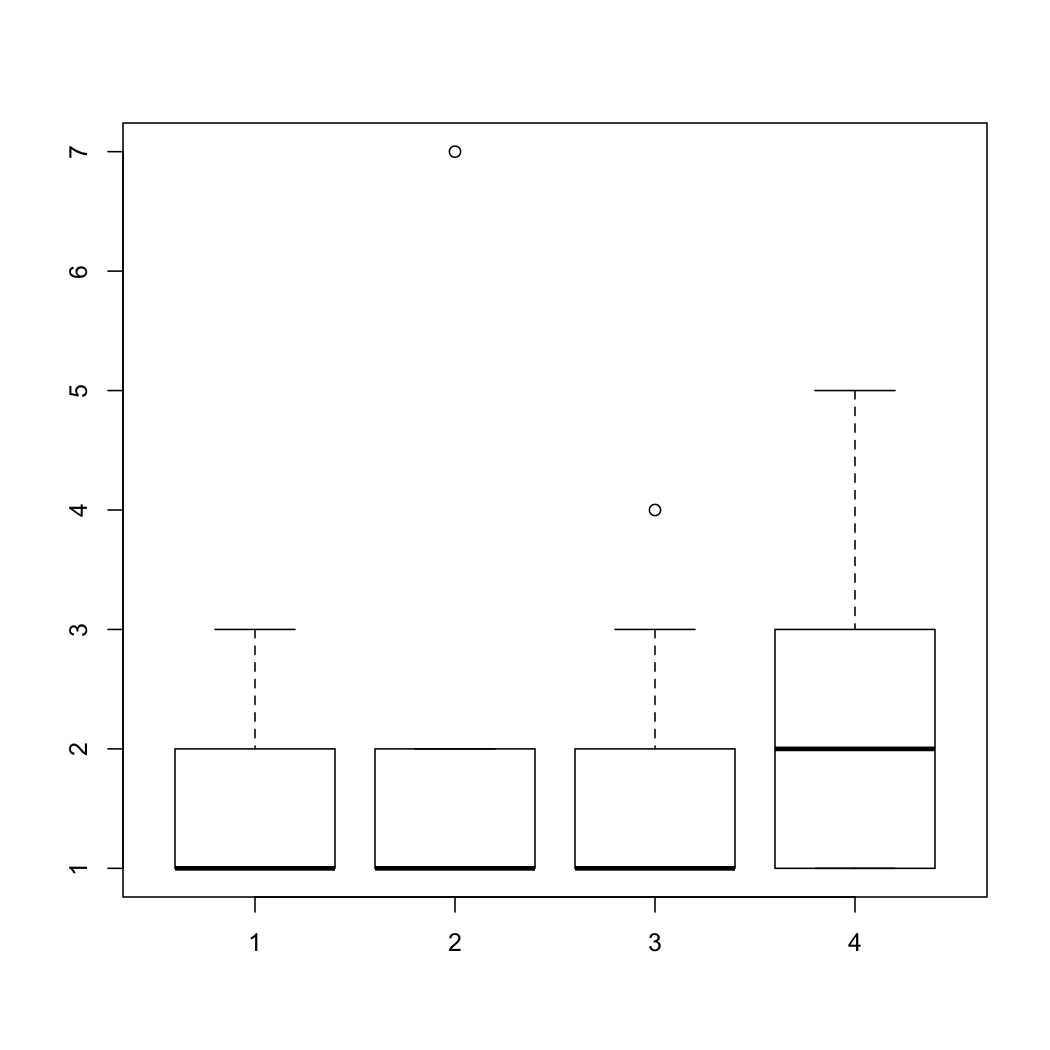
\includegraphics[height=2.5in]{img/Evaluierung/kollaboration.png}
	\caption{Verteilung der Benutzereinschätzungen zum kooperativen Modellieren}
	\label{fig:img_Evaluierung_kollaboration}
\end{figure}

In der qualitativen Befragung begründeten insgesamt 29 Teilnehmer ihren Eindruck (Fragestellung: „Sind Sie zufrieden mit ihrem Beitrag zum Modellierungsprozess? Geben Sie bitte auch eine kurze Begründung an.“). Die Ergebnisse sind im Folgenden inhaltlich gruppiert dargestellt:

\begin{itemize}
 \item pos: alle Teilnehmer haben Ideen eingebracht (6x)
 \item pos: gute Teamarbeit (5x)
 \item pos: konnte meine Ideen einbringen (5x)
 \item pos: Konsens gefunden (4x)
 \item pos: gute Kommunikation (3x)
 \item pos: alle Teilnehmer gleichgestellt (2x)
 \item neg: Werkzeug an Grenzen gestoßen (2x)
 \item neg: hatte zuwenig Wissen (1x)
 \item neg: Arbeit am Werkzeug war zu zeitaufwändig (1x)
\end{itemize}

Zudem konnten in der Videoanalyse der Evaluierungsblöcke 2, 3, 4 und 5 vielfach Situationen identifiziert werden, in denen das Modell auf der Tischoberfläche von den Teilnehmern als Referenz für den Austausch über die abgebildeten Inhalte herangezogen wurden oder in denen mehrere Teilnehmer gleichzeitig das Modell manipulierten. In der Folge werden prototypisch einige Situationen dargestellt, die derartige Interaktionsabläufe zeigen\footnote{Die ausgewählten Transkripte stammen aus Evaluierungsblock 3. Sämtliche Transkripte sind unter den in Anhang \ref{cha:daten_der_empirischen_untersuchung} angeführten Quellen zu beziehen.}:

\paragraph{Beispiel für gleichzeitige Manipulation} % (fold)
\begin{transkript}
	\textbf{A:} Sollen wir die beiden auch verbinden? \\
	\textbf{C:} Sicher. \emph{\textbf{(greift zu rotem Block)}} \\
	\textbf{A:} OK. \emph{\textbf{(greift zu blauem Block)}} \\
	\emph{\textbf{A und C schieben die Blöcke zusammen und anschließend wieder in die ursprüngliche Position. Anschließend setzt B den nächsten blauen Block auf die Arbeitsfläche, und verbindet ihn mit dem roten Block.}} \\
\end{transkript}

\paragraph{Beispiel für Referenzierung des Modells} % (fold)
\begin{transkript}
	\textbf{B:} Die Übung \emph{\textbf{(deutet auf roten Block)}} ist eigentlich nicht notwendig. \\
	\textbf{A:} Naja, es ist halt unter einem schönen Knoten. \\
	\textbf{C:} Nennen wir das \emph{\textbf{(tippt auf roten Block)}} Ziele. \\
	\textbf{A:} Nein, wieso? Ich kann ja mehrere Bedeutungen für das \emph{\textbf{(deutet auf roten Block)}} verwenden. Das ist doch egal. Das sagt ja nichts aus. \\
	\textbf{C:} Aber wir können das \emph{\textbf{(deutet auf roten Block)}} weggeben und sagen, das sind die Ziele. Was ist das Ziel. \\
	\textbf{A:} Das können wir machen, oder wir legen einfach einen roten dazu \emph{\textbf{(deutet an, wo der rote Block liegen würde)}} und schreiben es hin. \\
	\emph{A verschiebt den roten Block, um Platz für einen neuen Block zu schaffen.} \\
\end{transkript}

\paragraph{Beispiel für gleichzeitige Manipulation} % (fold)
\begin{transkript}
	\emph{Die Teilnehmer haben zuvor alle Blöcke beschriftet und wollen sie nun verbinden bzw. in die richtige Position bringen.} \\
	\textbf{B:} So und jetzt müssen wir eigentlich \ldots \emph{(greift zum ersten Block und schiebt ihn zum Knotenpunkt, um ihn zu verbinden, danach bringt er den Block wieder in seine ursprüngliche Position)} \\
	\textbf{C:} Jawohl. \\
	\emph{\textbf{Teilnehmer B wiederholt Vorgang mit dem zweiten Block. Teilnehmer C greift inzwischen zum dritten Block, um es B nachzumachen. B nimmt anschließend den nächsten Block und verbindet ihn. Den letzten Block verbindet wieder C.} Beim Zurückschieben verschwindet die Verbindung von der Arbeitsfläche.} \\
	\textbf{A:} Das erkennt er nicht. \emph{(schiebt den Block wieder ein Stück zurück)} \\
	\emph{System zeigt Verbindung wieder an.} \\
	\textbf{C:} Passt. \emph{Schiebt Block wieder zurück.} \\
	\textbf{A:} So, und jetzt noch schön anordnen. \\
	\emph{\textbf{A greift die unteren Blöcke und richtet sie in einer Linie aus, während C den ober Block zentriert.} System reagiert etwas verzögert. B lacht.} \\
	\textbf{A:} Ok. Passt. \\
	\emph{In der Folge beraten die Teilnehmer über die weitere Vorgangsweise.} \\
\end{transkript}

\paragraph{Beispiel für Referenzierung des Modells} % (fold)
\begin{transkript}
	\emph{Teilnehmer diskutieren über die beiden Modellierungssprachen.} \\
	\textbf{A:} In der Softwareentwicklung würde man das Analyse \emph{\textbf{(deutet auf oberen Teil der Arbeitsfläche)}} und das Design \emph{\textbf{(deutet auf unteren Teil der Arbeitsfläche)}} nennen. \\
	\textbf{B:} Genau. \\
	\textbf{A:} Und dann hinterlegst du es mit deinen mathematischen Modellen \emph{\textbf{(deutet Modelle mit Handbewegung an)}} in der Implementierung und dann kann ich es ausführen. \\
	\textbf{B:} Ja. Alles ablauforientiert das Ganze. \\
	\textbf{A:} \emph{\textbf{(deutet auf blauen Baustein)}} Genau, von der Sicht her. Die Sicht, die es einnimmt \emph{\textbf{(deutet auf gelbe Blöcke}}) ist genau dieselbe, aber der Scope vom Zeitpunkt ist genau. \\
	\textbf{B:} unterschiedlich \\
	\textbf{A:} Genau, SeeMe, ARIS \emph{\textbf{(deutet Modelle an)}} und dann Workflow Systeme im Wesentlichen. \\
\end{transkript}

\subsubsection{Diskussion} % (fold)

In der Verteilung der Zeitanteile der Beteiligung an der Modellierung zeigt sich, dass der Anteil von Teilnehmer A (dem Teilnehmer mit dem jeweils höchsten Zeitanteil) signifikant höher ist als jener von Teilnehmer B. In jenen Fällen, in denen drei Teilnehmer beteiligt sind, ist der Zeitanteil des am kürzesten beteiligten Teilnehmers signifikant geringer als jener der anderen beiden. Dieses Ergebnis scheint darauf hinzudeuten, dass für Anwendungssituationen mit mehreren Teilnehmern eine Beteiligung im gleichen Ausmaß nicht erwartet werden kann. Insgesamt spricht dieses Ergebnis also gegen die Bestätigung der Hypothese. 

Dies ist aber insofern zu relativieren, als dass eine statistisch signifikante Gleichverteilung nicht erwartet werden kann. Betrachtet man die Mittelwerte der Zeitanteile der Teilnehmer, so zeigt sich, dass -- zumindest für Anwendungen mit zwei Teilnehmern -- eine Beteiligung jeweils durch alle Teilnehmer gegeben ist. Der höhere Zeitanteil von Teilnehmer A ist unter Umständen auch auf den exklusiven Zugriff auf die zur Benennung von Modellierungsblöcken notwendige Tastatur zu erklären. Die Bedienung der Tastatur wurde nur in wenigen Fällen geteilt, so dass ein Teilnehmer durch die Durchführung der Benennungstätigkeit naturgemäß einen stärkeren Anteil an der Arbeitszeit in Anspruch nimmt. Bei drei Teilnehmern zeigt sich jedoch eine deutliche Abnahme des Zeitanteils für jenen Teilnehmer, der den geringsten Zeitanteil in Anspruch nahm. Dieser Effekt verstärkt sich -- wie aus Beobachtungen der Anwendungen in Evaluierungsblock 4 zu erkennen (siehe \citep{Wahlmuller10}) -- für Anwendungen mit mehr als drei Teilnehmern. Hier sind jeweils tendenziell zwei Beteiligte zu identifizieren, die zusammen mehr als zwei Drittel der Modellierungszeit für sich in Anspruch nehmen.  

In der Befragung der Benutzer hinsichtlich der wahrgenommenen Möglichkeit zur Kooperation wird deutlich, dass diese durchwegs als hoch eingeschätzt wird (dies gilt sowohl für die Anwendungen mit zwei Teilnehmern in Block 5 als auch für die Anwendungen mit drei und mehr Teilnehmern in Block 4). Auch in den qualitativen Rückmeldungen zur Kooperation wird das Werkzeug hinsichtlich seiner Wirkung positiv beurteilt. Die Antworten auf die offenen Fragestellungen zeigen ebenfalls eine vorwiegend positive Einschätzung der Wirkung des Werkzeugs auf die Kooperation zwischen den Teilnehmern. Das Ergebnis der Befragung spricht also insgesamt für die Bestätigung der Hypothese.

Auch die Ergebnisse der Videoanalyse deuten auf eine kooperationsunterstützende Wirkung des Werkzeugs hin. Zu nennen ist hierbei vor allem die vielfache Verwendung der Modellelemente als physischer Ankerpunkt, an dem Diskussionbeiträge durch Zeigen oder Deuten festgemacht werden und so den anderen Teilnehmern der Bezugsgegenstand verdeutlicht wird. Dieses Verhalten bei der Modellbildung war in der vergleichenden Anwendung der rein rechnerbasierten CMapTools in Evaluierungsblock 5 in weitaus geringerem Ausmaß zu beobachten. Auch die simultane Manipulation am Modell durch mehrere Teilnehmer trat wiederholt auf. Dabei handelte es sich selten um vollständig voneinander entkoppelte Aktivitäten, in den meisten Fällen wurde simultan jener Modellteil manipuliert, der aktuell Gegenstand der Diskussion war. Durch die bei rein rechner-gestützten Modellierungswerkzeugen exklusiven Interaktionsmöglichkeit durch die Maus ist dieses Verhalten dort nicht zu beobachten und deutet auf einen auf das Werkzeug zurückzuführenden Effekt hin.   

Insgesamt kann die hier untersuchte Hypothese auf Basis der durchgeführten Untersuchungen deshalb bestätigt werden.

\subsubsection{Ergebnis} % (fold)

\textbf{Hypothese \ref{hyp:kollaborativ} kann auf Basis der Untersuchung bestätigt werden.} Der Zeitanteil an der Modellbildung zeigt bei Anwendungen mit zwei Modellierenden eine wesentliche Beteiligung jeweils beider Teilnehmer. Bei mehr als zwei Anwendern ist die Beteiligung aller Teilnehmer nicht mehr gegeben, die Teilnehmer haben dennoch durchwegs (unabhängig von der Anzahl der Teilnehmer bei einer Anwendung) den Eindruck, sich einbringen zu können und gut zusammenarbeiten zu können.

% subsection kollaboratives_arbeiten (end)

\subsection{Einsetzbarkeit in unterschiedlichen Kontexten} % (fold)
\label{sub:einsetzbarkeit_in_unterschiedlichen_kontexten}

Gegenstand der hier beschriebenen Untersuchung ist Hypothese \ref{hyp:kontexte} („Das Werkzeug ist gleichwertig für Modellierungsaufgaben in unterschiedlichen Kontexten einsetzbar.“). Als Grundlage dieser Untersuchung dienen die Ergebnisse der Evaluierungsblöcke 2, 3, 4 und 5. Die Anwendungskontexte unterscheiden sich weitgehend zwischen den Blöcken. In Block 2 werden Ablaufplanungen im universitären Lern-Kontext behandelt, die Blöcke 3 und 5 bilden Aufgaben zur Reflexion von Lerninhalten ab. Block 4 zeigt den Einsatz des Werkzeugs im organisationalen Kontext, wobei hier sowohl die Aufbau- als auch die Ablauforganisation (zumeist nicht trennbar) behandelt wurden. Zur Auswertung werden also drei Kontexte (Block 2, Blöcke 3 und 5 sowie Block 4) betrachtet. In den Blöcken 4 und 5 wurden die Teilnehmer zusätzlich hinsichtlich der Zufriedenheit mit der Abbildung ihrer mentalen Modelle befragt. Auch diese Ergebnisse dienen der Prüfung dieser Hypothese.

\subsubsection{Auswertung} 

Im quantitativen Teil der hier durchgeführten Auswertung wurde die Korrelation zwischen der Modellierungszeit und der Modellgröße in den unterschiedlichen Evaluierungsblöcken berechnet. Abbildung \ref{fig:img_Evaluierung_correlation} zeigt den Zusammenhang graphisch.

\begin{figure}[htbp]
	\centering
		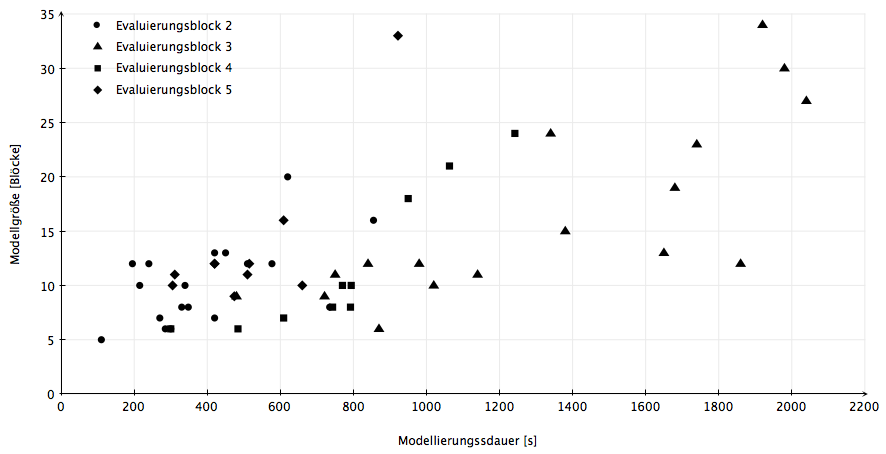
\includegraphics[width=15cm]{img/Evaluierung/correlation.png}
	\caption{Zusammenhang zwischen Modellgröße und Modellierungsdauer}
	\label{fig:img_Evaluierung_correlation}
\end{figure}

Über alle Evaluierungsblöcke hinweg ($n=57$) ergibt sich mit einem Korrelationskoeffizient nach Spearman\footnote{Der Korrelationskoeffizient nach Pearson kann nicht angewandt werden, da beide Stichproben nicht normalverteilt sind (Shapiro-Wilk-Test: $W_{Zeit}=0.880, p_{Zeit}<0.005$, $W_{Größe}=0.829, p_{Größe}<0.005$)} von $0.60019$ ein signifikant positiver Zusammenhang zwischen den beiden Messgrößen (Test auf positive Korrelation: $S=11082.87, p<0.005$).

Bei der Befragung der Benutzer in den Blöcken 4 ($n=13$) und 5 ($n=24$) wurde unter anderem deren Zufriedenheit mit dem Modellierungsergebnis sowie der Anwendung der Werkzeugs zur Lösung der Aufgabenstellung qualitativ erhoben. In Evaluierungsblock 4 gaben 11 Teilnehmer an, mit dem Modellierungsergebnis zufrieden gewesen zu sein. Ein Teilnehmer war unzufrieden, einer beantwortete die Frage nicht. Insgesamt wurden von 9 Teilnehmern Begründungen angegeben, die im Folgenden inhaltlich gruppiert dargestellt sind:

\begin{itemize}
	\item pos: kooperatives Arbeiten möglich (3x)
	\item pos: neue Erkenntnisse gewonnen (2x)
	\item pos: Ergebnis entspricht den Vorstellungen (2x)
	\item neg: zu große Teile, zu kleine Oberfläche (2x)
\end{itemize}

11 Teilnehmer gaben an, mit dem Modellierungsverlauf zufrieden gewesen zu sein, ein Teilnehmer war nicht zufrieden, ein Teilnehmer beantwortete die Frage nicht. Insgesamt wurden von 8 Teilnehmern Begründungen angegeben, die im Folgenden inhaltlich gruppiert dargestellt sind:

\begin{itemize}
	\item pos: kooperatives Arbeiten möglich (3x)
	\item pos: Kommunikation gefördert, gemeinsame Sichtweise entwickelt (2x)
	\item pos: Experimentieren ist möglich (1x)
	\item pos: spielerisches Modellieren möglich (1x)
	\item neg: zu große Teile, zu kleine Oberfläche (1x)
	\item neg: Werkzeug ist umständlich (1x)
	\item neg: Werkzeug technisch instabil (1x)
\end{itemize}

In Evaluierungsblock 5 gaben 18 Teilnehmer an, mit dem Modellierungsergebnis zufrieden gewesen zu sein. 6 Teilnehmer waren unzufrieden. 23 Teilnehmer begründeten ihre Entscheidung. Die Begründungen sind im Folgenden inhaltlich gruppiert dargestellt:

\begin{itemize}
	\item pos: Modell war vollständig (5x)
	\item pos: Aufgabe gut gelöst (5x)
	\item pos: Modell war verständlich (2x)
	\item pos: Ergebnis entspricht den Vorstellungen (2x)
	\item pos: rasche Modellierung war möglich (1x)
	\item neg: Werkzeug technisch instabil (4x)
	\item neg: Modell war zu ungenau (3x)
	\item neg: Modell war unübersichtlich (2x)
\end{itemize}

20 Teilnehmer gaben an, mit dem Modellierungsverlauf zufrieden gewesen zu sein, 4 Teilnehmer waren nicht zufrieden. Alle 24 Teilnehmer begründeten ihre Entscheidung. Die Begründungen sind im Folgenden inhaltlich gruppiert dargestellt:

\begin{itemize}
	\item pos: kooperatives Arbeiten möglich (11x)
	\item pos: Kommunikation gefördert (7x)
	\item pos: Werkzeug einfach zu bedienen (5x)
	\item pos: Verwendung unterhaltsam (3x)
	\item pos: zügiges Arbeiten möglich (3x)
	\item pos: gute Aufgabenteilung (1x)
	\item neg: Werkzeug technisch instabil (3x)
	\item neg: Werkzeug ist umständlich (1x)
	\item neg: unstrukturiertes Vorgehen (1x)
\end{itemize}

\subsubsection{Diskussion} 

Der Korrelationskoeffizient zwischen Modellgröße und Modellierungsdauer deutet bei einer Berechnung über alle Evaluierungsblöcke hinweg mit einem Wert von $0.600$ auf eine signifikant positive Korrelation zwischen diesen beiden Parametern hin. Da damit unabhängig von der Modellierungsaufgabe offensichtlich ein Zusammenhang zwischen den geprüften Parametern besteht, stützt dies die Hypothese, dass sich das Werkzeug für den Einsatz in unterschiedlichen Kontexten eignet. Auch die in Abschnitt \ref{sub:gewöhnung_an_das_werkzeug} verwendeten „normierten“ Modellierungszeiten (Modellierungdauer im Verhältnis zur Modellgröße, also im Wesentlichen Zeitaufwand pro Block) zeigen für die dort gegenübergestellten Blöcke 2 und 3 keinen signifikanten Unterschied im Aufwand bei der Modellierung, obwohl die Anwendungen aus unterschiedlichen Kontexten stammen.

Bei der qualitativen Betrachtung der Rückmeldungen der Benutzer hinsichtlich der Zufriedenheit mit dem Modellierungsverlauf und Ergebnis zeigen sich unabhängig von jeweiligen Anwendungskontext überwiegend positiv zu wertende Rückmeldungen. Betrachtet man die mehrfach genannten Begründungen der Einschätzungen, gleichen sich sowohl die positiven als auch die negativen Rückmeldungen in den beiden Anwendungskontexten. Dies spricht für die Bestätigung der untersuchten Hypothese.

Zusammenfassend kann Hypothese \ref{hyp:kontexte} also auf Basis der Ergebnisse der durchgeführten Untersuchungen bestätigt werden.

\subsubsection{Ergebnis} 

\textbf{Hypothese \ref{hyp:kontexte} kann auf Basis der Untersuchung bestätigt werden.} Die quantitative Untersuchung der Korrelation zwischen Modellgröße und Modellierungsdauer zeigt unabhängig vom Anwendungskontext eine signifikant positive, relativ stark ausgeprägte Korrelation, was darauf hinweist, dass der Aufwand zur Modellerstellung unabhängig von Aufgabenstellung und Anwendungskontext relativ stabil bleibt. Auch die qualitativen Rückmeldungen der Teilnehmer aus unterschiedlichen Anwendungskontexten gleichen sich im Wesentlichen, so dass das Werkzeug unabhängig vom Anwendungskontext immer ähnliche positive bzw. negative Effekte zu haben scheint.

% subsection einsetzbarkeit_in_unterschiedlichen_kontexten (end)

\subsection{Wiederherstellung vergangener Modellzustände} % (fold)
\label{sub:wiederherstellung_vergangener_modellzustände}

Gegenstand der hier beschriebenen Untersuchung ist Hypothese \ref{hyp:wiederherstellung} („Die Möglichkeit der Wiederherstellung vergangener Modellzustände fördert die Bereitschaft alternative Repräsentationen auszuprobieren.“). Als Grundlage dieser Untersuchung dienen die Ergebnisse der Evaluierungsblöcke 2 bis 5, da die Funktion zur Wiederherstellung vergangener Modellzustände erst in diesen Blöcken funktionsfähig zur Verfügung stand.

\subsubsection{Auswertung} 

Für alle Anwendungen des Werkzeugs in den Evaluierungsblöcken 2 bis 5 wurde hier untersucht, wie oft die Möglichkeit zur Wiederherstellung vergangener Modellzustände eingesetzt wurde, um alternative Modellierungswege auszuprobieren. Nicht berücksichtigt wurden Einsätze derselben Funktion, die zur Korrektur von Modellierungsfehlern durch Fehl-Erkennungen des Systems verwenden wurden (verstärkt in den Evaluierungsblöcken 2 und 3 aufgetreten, in 4 und 5 durch Stabilisierung der Erkennungsleistung nicht mehr relevant -- siehe Abschnitt \ref{sub:verwendung_des_löschtokens}). Die Verteilung des Einsatzes der Funkion ist in absoluten Zahlen in Tabelle \ref{tab:anzahl_wiederherstellung} für jeden Evaluierungsblock angeführt

\begin{table}[htbp]
	\centering
	\caption{Anzahl des Einsatzes der Wiederherstellungsfunkion}
\begin{tabular}{| c || c | c | c | c |}
  \hline
   EB    & 0 E. & 1 E. & 2 E. & 3+ E. \\ \hline
   2     & 18 & 0 & 0 & 0 \\ 
   3     & 14 & 4 & 0 & 0 \\ 
   4     & 10 & 0 & 0 & 0 \\ 
   5     & 10 & 1 & 0 & 0 \\ \hline
   Ges.  & 52 & 5 & 0 & 0 \\ \hline
\end{tabular} \\
\footnotesize EB \ldots Evaluierungsblock, x E.\ldots x Einsätze der Wiederherstellungsfunktion
	\label{tab:anzahl_wiederherstellung}
\end{table}

Die Wiederherstellungsfunktion wurde also insgesamt in $8.77\%$ der Fälle ($n=57$) eingesetzt und kam maximal einmal je Anwendung zum Einsatz.  Aus den Videoanalysen ist außerdem erkennbar, dass die Wiederherstellungsfunktion -- falls ihre Verwendung überhaupt in Betracht gezogen wird -- in den meisten Fällen lediglich zur Fehlerkorrektur eingesetzt wird (in 52 Anwendungen wurde die Wiederherstellungsfunkion in 37 Fällen -- $71.2\%$ -- mindestens einmal zur Korrektur von Erkennungsfehlern und 5 mal zur Korrektur von inhaltlich verworfenen Modellierungswegen verwendet).

Bei der in den Blöcken 1, 4 und 5 durchgeführten Befragung der Teilnehmer hinsichtlich der Erfahrungen mit dem Werkzeug wurde unter anderem nach als besonders nützlich empfundenen Funktionen bzw. Eigenschaften des Werkzeugs gefragt. Die Wiederherstellungsfunktion wurde in diesem Zusammenhang von keinem Teilnehmer ($n=55$) erwähnt. 

\subsubsection{Diskussion} 

Die Ergebnisse der Auswertung der Untersuchung zu dieser Hypothese zeigt ein geringes Ausmaß der Verwendung der Wiederherstellungsfunktion zum Zwecke der Erstellung von Modellalternativen. Die Funktion an sich wurde in $71.2\%$ der Anwendungen verwendet, was für ein hohes Bewusstsein über deren Existenz spricht. Lediglich in $8.77\%$ der Anwendungen wurde die Funktion zur Verfolgung alternativer Modellierungswege eingesetzt, in $61.5\%$ der Anwendungen wurde sie lediglich zur Fehlerkorrektur verwendet. Auch in der qualitativen Erhebung der als nützlich wahrgenommenen Werkzeugfunktionalitäten wurde die Wiederherstellungsfunktion in keinem Fall genannt. Auf Basis dieser Ergebnisse kann die Hypothese nicht bestätigt werden. 

\subsubsection{Ergebnis} 

\textbf{Hypothese \ref{hyp:wiederherstellung} kann auf Basis der Untersuchung nicht bestätigt werden.} Die Wiederherstellungsfunktion wird nur in unter $10\%$ der untersuchten Anwendungen  zur Verfolgung alternativer Modellierungswege genutzt. Die Funktion wird außerdem von den Anwendern bei der Frage nach den als nützlich wahrgenommene Funktionen nicht genannt.

% subsection wiederherstellung_vergangener_modellzustände (end)

\subsection{Nicht-Behinderung} % (fold)
\label{sub:nicht_behinderung}

Gegenstand der hier beschriebenen Untersuchung ist Hypothese \ref{hyp:behinderung} („Das Werkzeug behindert die Modellbildung nicht.“). Als Grundlage dieser Untersuchung dienen die Ergebnisse der Evaluierungsblöcke 2 bis 5, da sich das Werkzeug erst in diesen Blöcken hinsichtlich der Funktionalität in vollständigem Zustand befand. Zu berücksichtigen ist bei der Auswertung, dass im Laufe der Evaluierungsblöcken 4 und 5 eine Überarbeitung der Implementierung vorgenommen wurde, mittels der das Auftreten von Fehl-Erkennungen verringert werden konnte und deren Korrektur weniger aufwändig wurde. Befragungen der Modellierenden hinsichtlich einer etwaigen Behinderung durch das Werkzeug wurden in den Blöcken 1, 4 und 5 durchgeführt, wobei lediglich die Anmerkungen aus den letzen beiden Blöcken für den aktuellen Entwicklungsstand des Werkzeugs relevant sind.

\subsubsection{Auswertung} 

In Tabelle \ref{tab:fehlfunktionen} wird gegliedert nach Evaluierungsblöcken dargestellt, wie oft es in einer einzelnen Anwendung zu Fehlfunktionen in der Erkennung kam, die den Modellierungsfluss unterbrachen. Als Fehl-Erkennungen wurde das Verschwinden von Blöcken oder Fehlzuordnungen von Benennungen sowie die unbeabsichtigte oder von System eigenständig vorgenommene Erstellung oder Entfernung von Verbindern bzw. Richtungspfeilen eingeordnet. Zusätzlich wurden Systemabstürze als massive Unterbrechung, die zum Gesamtverlust des bis zum Zeitpunkt des Absturzes erstellten Modells führten, separat ausgewertet.

\begin{table}[htbp]
	\centering
	\caption{Fehlfunktionen und Abstürze des Werkzeugs}
\begin{tabular}{| c || c || c | c | c | c || c |}
  \hline
   EB    & Anw. & 0 Ff. & 1-3 Ff. & 4-6 Ff. & 7+ Ff. & Systemabstürze \\ \hline
   2     & 18 & 0 &  8 &  5 &  5 &  4 \\ 
   3     & 18 & 1 & 10 &  4 &  3 &  5 \\ 
   4     & 10 & 0 &  2 &  2 &  5 &  1 \\ 
   5     & 11 & 0 &  3 &  3 &  4 &  5 \\ \hline
   Ges.  & 57 & 1 & 23 & 14 & 17 & 15 \\ \hline
\end{tabular} \\
\footnotesize EB \ldots Evaluierungsblock, Anw. \ldots Anzahl der Anwendungen, x Ff.\ldots x Fehlfunktionen
	\label{tab:fehlfunktionen}
\end{table}

In der Gesamtheit der betrachteten Anwendungen ($n=57$) ergibt sich die in Tabelle \ref{tab:fehlfunktionen} dargestellte Verteilung der Anzahl der Fehlerkennungen je Anwendung, die auch in Abbildung \ref{fig:img_Evaluierung_fehlerkennungen} graphisch abgebildet ist. In $1.75\%$ der Fälle trat keine Fehlerkennung während der Anwendung auf ($n_{0}=1$). In $40.35\%$ der Fälle traten zwischen 1 und 3 Fehlerkennungen auf ($n_{1-3}=23$). 4-6 Fehlerkennungen konnten in $24.56\%$ der Fälle festgestellt werden ($n_{4-6}=14$). 7 oder mehr Fehlerkennungen traten in $29.82\%$ der Fälle auf ($n_{7+}=17$). In $26.32\%$ der Fälle kam es zu Systemabstürzen ($n_{Absturz}=15$), wobei diese in 10 Fällen nach Ende des eigentlichen Modellierungsvorgangs auftraten.

\begin{figure}[htbp]
	\centering
		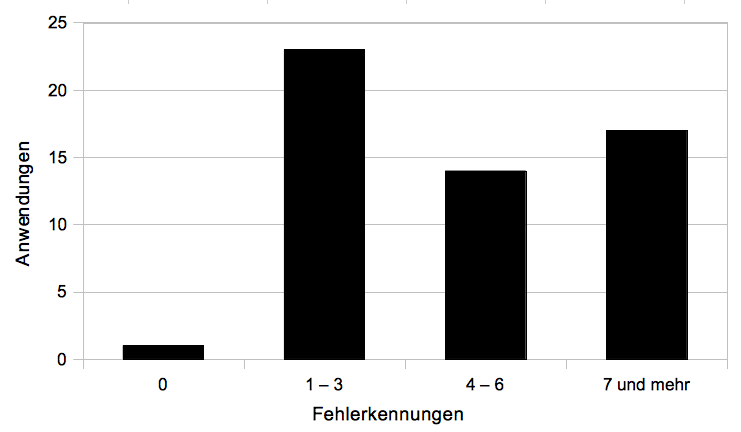
\includegraphics[width=10cm]{img/Evaluierung/fehlerkennungen.png}
	\caption{Verteilung der Anzahl der Fehlerkennungen je Anwendung -- Übersicht}
	\label{fig:img_Evaluierung_fehlerkennungen}
\end{figure}

In der Benutzerbefragung in den Evaluierungsblöcken 4 und 5 wurde in offenen und geschlossenen Fragen nach der Wirkung des Werkzeugs bei der Modellbildung befragt (Abschnitte „Nutzerfreundlichkeit“ und „Zufriedenheit des Modellierers“ in Block 4 -- siehe Anhang \ref{sub:fb_eval4} -- und Abschnitte „wahrgenommene Einfachheit der Benutzung des Werkzeugs“ und „Zufriedenheit des Modellierers“ in Block 5 -- siehe Anhang \ref{sub:fb_eval5}). Die für die Prüfung der hier betrachteten Hypothese sind folgende geschlossene Items relevant:

\begin{enumerate}
	\item Die Anwendung des Werkzeugs ist frustrierend (Skala gedreht).
	\item Die Anwendung des Werkzeugs fällt mir leicht.
	\item Die Anwendung des Werkzeugs ist anstrengend (Skala gedreht).
	\item Um mit dem Werkzeug gut zurecht zu kommen, hätte ich intensivere Vorbereitung benötigt (Skala gedreht).
	\item Die Bedienung des Werkzeugs ist intuitiv.
	\item Das Werkzeug ist einfach zu bedienen.
	\item Die benötigte Zeit um das Modell zu erstellen empfand ich als angemessen.
\end{enumerate}

Insgesamt wurden $n=37$ Teilnehmer befragt. Die Ergebnisse sind in Tabelle \ref{tab:behinderung} und Abbildung \ref{fig:img_Evaluierung_behinderung} zusammengefasst dargestellt. Neben dem Mittelwert und der Standardabweichung wurde für jedes Item auch geprüft, ob die Einschätzung als signifikant positiv zu bezeichnen ist. Dazu wurde ein einseitiger Wilcoxon-Test für die Stichprobe gegenüber dem Skalenmittelwert 4 durchgeführt\footnote{Der Wilcoxon-Test muss angewandt werden, da die Stichprobe in allen sieben Fällen nicht normalverteilt ist (Shapiro-Wilk-Test: $W_{1}=0.877, p{1}<0.005$, $W_{2}=0.798, p{2}<0.005$, $W_{3}=0.871, p{3}<0.005$, $W_{4}=0.764, p{4}<0.005$, $W_{5}=0.862, p{5}<0.005$, $W_{6}=0.833, p{6}<0.005$, $W_{7}=0.844, p{7}<0.005$)}.

\begin{table}[htbp]
	\centering
	\caption{Befragung über die Wirkung des Werkzeugs -- Itemauswertung}

\begin{tabular}{| c || c | c || c | c |}
  \hline
   Item & M & SD & $V_{M<4}$ & $p_{M<4}$ \\ \hline
   1* & $2.89$ & $1.76$ & $100$ & $<0.005$ \\ 
   2  & $2.19$ & $1.29$ & $20$ & $<0.005$ \\ 
   3* & $2.65$ & $1.49$ & $49$ & $<0.005$ \\ 
   4* & $2.08$ & $1.28$ & $33.5$ & $<0.005$ \\ 
   5  & $2.78$ & $1.49$ & $70.5$ & $<0.005$ \\ 
   6  & $2.32$ & $1.21$ & $27$ & $<0.005$ \\ 
   7  & $2.16$ & $1.35$ & $20.5$ & $<0.005$ \\ \hline
\end{tabular} \\ 
	\footnotesize * \ldots Item gedreht
	\label{tab:behinderung}
\end{table}

\begin{figure}[htbp]
	\centering
		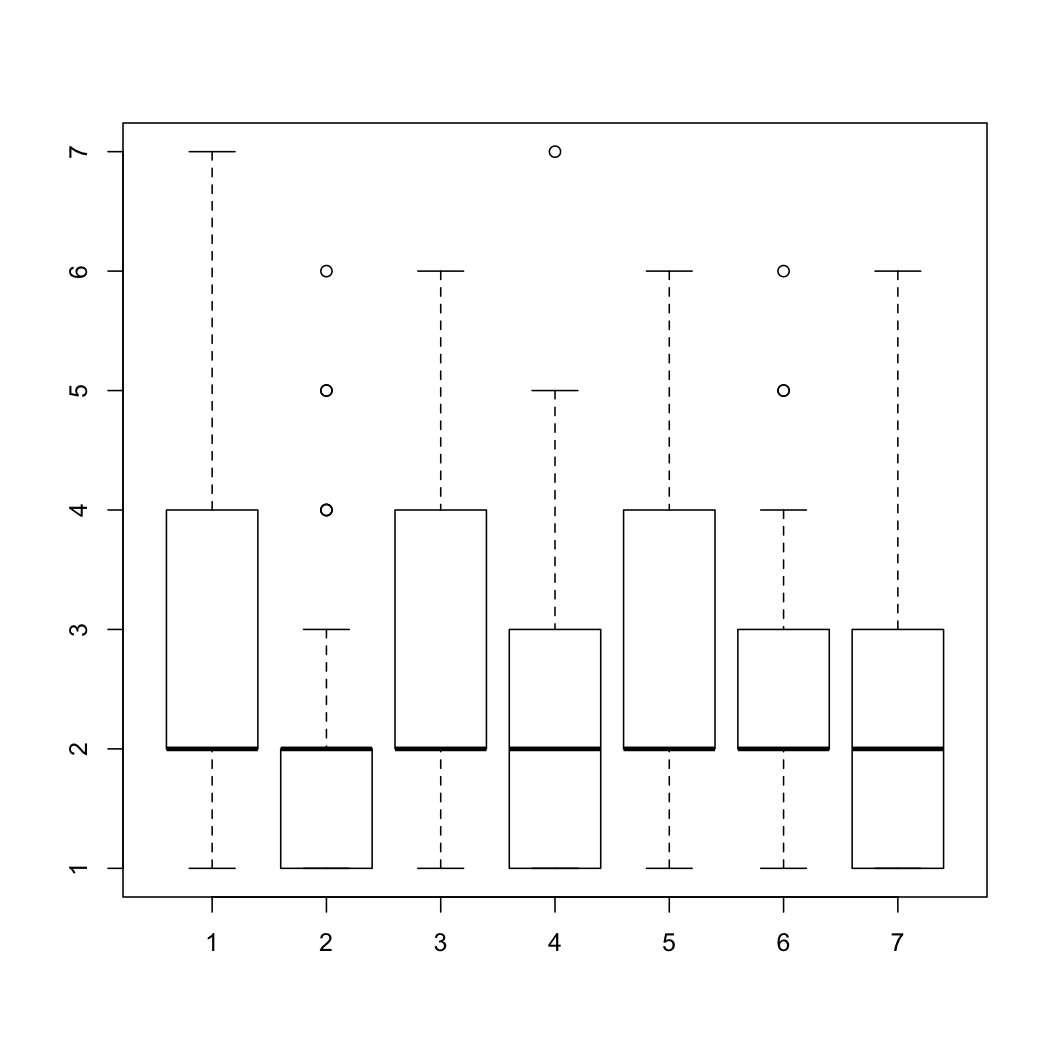
\includegraphics[height=3in]{img/Evaluierung/behinderung.png}
	\caption{Verteilung der Benutzereinschätzungen zur Wirkung des Werkzeugs}
	\label{fig:img_Evaluierung_behinderung}
\end{figure}

In der qualitativen Befragung gaben insgesamt 34 Teilnehmer Rückmeldungen zur Bedienung des Werkzeugs ab (Fragestellung: „Wie zufrieden waren sie im Allgemeinen mit dem Werkzeug?“). Die Ergebnisse sind im Folgenden inhaltlich gruppiert dargestellt:

\begin{itemize}
 \item pos: Prototypen-Probleme nicht überbewerten, trotzdem verwendbar (7x)
 \item pos: intuitive Herstellung von Verbindern möglich (2x)
 \item pos: Benutzung war spannend und nützlich (2x)
 \item pos: Hinweise zum Wiederherstellen eines Zustandes (2x)
 \item pos: ermöglicht das spielerische Nachdenken über Prozesse (1x)
 \item pos: Interaktion mit dem Werkzeug einfach möglich (1x)
 \item pos: Anfassbarkeit verstärkt die Beziehung zum Thema (1x)
 \item neg: Objekte zu groß / Oberfläche zu klein (9x)
 \item neg: System zu instabil (8x)
 \item neg: System zieht tw. selbständig Verbindungen (4x)
 \item neg: Erkennungsleistung in Teilbereichen mangelhaft (3x)
 \item neg: zu wenig Verbinder-Varianten (3x)
 \item neg: zu wenig Baustein-Varianten (2x)
 \item neg: Beschriftung unterbricht den Modellierungsfluss (1x)
 \item neg: Tisch zu hoch (1x)
 \item neg: System umständlich zu bedienen (1x)
 \item neg: zu träge Reaktion (1x)
\end{itemize}

In der Videoanalyse der Evaluierungsblöcke 2, 3, 4 und 5 konnten Situationen identifiziert werden, die die am häufigsten genannten negativen Wirkungen des Werkzeugs bestätigen. In der Folge werden prototypisch einige Situationen dargestellt, die derartige Interaktionsabläufe zeigen, in denen die Bedienung des Werkzeugs behindert wird\footnote{Die ausgewählten Transkripte stammen aus Evaluierungsblock 3. Sämtliche Transkripte sind unter den in Anhang \ref{cha:daten_der_empirischen_untersuchung} angeführten Quellen zu beziehen.}:

\paragraph{Oberfläche zu klein} 

\begin{transkript}
\emph{Teilnehmer A will einen neuen Block hinzufügen, hat aber wenig Platz.} \\
\emph{A setzt gelben Block an den unteren Rand der Arbeitsfläche.} \\
\textbf{B:} \textbf{Geben wir ihn hier rauf. \emph{(schiebt Blöcke zur Seite)} Sonst können wir sie nicht verbinden.} \\
\textbf{C:} Stimmt. \\
\emph{A setzt Block auf die freigelegte Fläche. B und C schieben inzwischen die anderen Blöcke auseinander, um noch mehr Platz zu schaffen. C setzt den Marker zum neuen Baustein. A beschriftet. C nimmt den Marker weg.} \\
\emph{Die Teilnehmer setzen mit dem verbinden der Blöcke ihre Arbeit fort.} \\
\end{transkript}

\paragraph{System zu instabil - Fall 1}

\begin{transkript}
\emph{B stellt blauen Block auf die Arbeitsfläche und schiebt ihn zum roten Block. System erstellt jedoch keine Verbindung.} \\
\textbf{A:} Egal, dann fahren wir mit dem Roten weiter rauf. \emph{(Nimmt roten Block und schiebt ihn in Richtung blauen Block den TLN B auf der Arbeitsfläche bewegt)} \textbf{Jetzt erkennt er das auch nicht mehr \emph{(meint Verbindung, die kurz verschwindet)}}. \\
\emph{Die beiden schieben die Blöcke gleichzeitig wieder in Richtung der Ausgansposition.} \\ \emph{\textbf{Verschwundene Verbindung wird wieder angezeigt. Neue Verbindung wird nicht erkannt.}} \\
\textbf{A:} Egal. \emph{(schiebt roten Block nach links oben, während B den blauen Block nach rechts unten hebt)} \\
\textbf{A:} Versuchen wir es hier einmal. \\
\emph{B schiebt den blauen Block nach links oben zum roten Block zurück. System erkennt die Verbindung. B schiebt den Block nach rechts unten zurück und \textbf{A verschiebt den roten Block, weil die Verbindungen kurz verschwunden sind}. Teilnehmer setzen mit der Modellierung fort.}
\end{transkript}

\paragraph{System zu instabil - Fall 2}

\begin{transkript}
\emph{\textbf{Das System hat einen ungewollten Verbinder erstellt.}} \\
\emph{B stellt das Glas auf die Oberfläche und dreht es} \\
\textbf{A:} jetzt ist es weg! \\
\emph{B hebt das Glas von der Oberfläche, ohne das Wiederherstellungskärtchen zu verwenden} \\
\emph{Beide Teilnehmer verharren kurz ohne zu sprechen} \\
\textbf{B:} nein, he, hallo \\
\emph{B setzt das Glas wieder auf die Oberfläche} \\
\emph{A murmelt unverständlich, das letzte Wort scheint vielleicht zu sein} \\
\emph{B dreht das Glas, nimmt die Hand vom Glas und tippt kurz mit den Fingern auf die Oberfläche} \\
\textbf{B:} OK, und jetzt? \\
\textbf{A:} Wenn du es weg tust, ist es wieder \\
\emph{B greift zu einem Marker} \\
\textbf{B:} commiten! \\
\emph{B setzt den Marker zweimal kurz auf die Tischoberfläche und nimmt ihn danach vom Tisch} \\
\textbf{B:} nein \\
\emph{\textbf{A murmelt unverständlich und zeigt auf den ungewollten Verbinder, der noch immer besteht}} \\
\emph{B hebt das Glas kurz an und stellt es wieder auf die Oberfläche} \\
\textbf{B:} ah geh, ich frage ihn gleich \\
\emph{B verlässt den den Raum und ruft den Seminarleiter herbei, um ihnen bei dem Problem behilflich zu sein} \\
\end{transkript}

\paragraph{System zu instabil - Fall 3}

\begin{transkript}
\emph{Das System hat einen ungewollten Verbinder erstellt. Die Teilnehmer wollen diesen mit dem Glas entfernen.} \\
\emph{B nimmt das Glas und das Kärtchen gleichzeitig vom Tisch} \\
\textbf{B:} geh nein, nicht das weg tun \\
\emph{\textbf{Das System scheint einen blauen Block am linken unteren Ende der Oberfläche verloren zu haben}} \\
\textbf{B:} wah \emph{(frustriert)} \\
\textbf{B:} gibt es ja nicht \\
\emph{B nimmt den nicht mehr erkannten blauen Block von der Oberfläche} \\
\textbf{B:} OK, weg tun \\
\textbf{B:} Was ist jetzt da verkehrt? \\
\emph{B greift zu einem roten Block, das System zeigt mit einer grünen gefüllten Ellipse an, er solle den Block etwas verschieben, er berührt den Block leicht und verschiebt ihn minimal, das System erkennt dies und fordert die Teilnehmer auf, einen weiteren Block zu verschieben. Die Teilnehmer können dies nicht deuten. B nimmt den Block der verschoben werden sollte von der Oberfläche und stellt ihn wieder ab, allerdings neben der markierten Zielposition. \textbf{B greift zu dem zuvor entfernten blauen Block und legt ihn wieder an seine ursprüngliche Position, das System reagiert nicht darauf.}} \\
\textbf{A:} vielleicht einmal die \\
\emph{A greift zu dem obersten roten Block und verschiebt diesen weiter nach oben, er verschiebt auch weitere rote Blöcke, einen dieser Blöcke verschiebt er auf die grün gefüllte Ellipse. Es handelt sich dabei jedoch um den falschen Block.} \\
\emph{\textbf{Das System scheint einen ungewollten Verbinder erstellt zu haben}} \\
\textbf{A:} jetzt hat er da wieder eine Verbindung gemacht \\
\textbf{B:} warte, drehen wir nochmal zurück \\
\emph{B greift zu dem Glas (außerhalb des Bildbereichs)} \\
\textbf{B:} \textbf{Da bist du mit den Nerven fertig, bevor du irgendetwas zusammengebracht hast, was passt} \\
\emph{Die Teilnehmer setzen die Modellierung fort, das System verlangt noch immer, dass die Teilnehmer einen roten Block an seinen richtigen Platz schieben und zeigt die von den Teilnehmern durchgeführten Änderung nicht an.} \\
\end{transkript}

\paragraph{System zieht selbständig Verbindungen}

\begin{transkript}
\emph{Das System hat eine unerwünschte Verbindung erstellt.} \\
\emph{B schiebt die beiden Blöcke mit der ungewollten Verbindung aneinander} \\
\textbf{B:} \textbf{OK, jetzt haben wir wirklich eine Verbindung, die müssen wir wieder löschen} \\
\textbf{A:} hm? \\
\textbf{B:} oder? \\
\textbf{A:} Was willst du denn löschen? \\
\textbf{B:} ja die Verbindung \\
\textbf{A:} wieso? \\
\textbf{B:} zeigt auf die Verbindung – brauchen wir da eine? \\
\textbf{A:} ja, wieso? Sicher \\
\textbf{B:} \emph{(unverständlich)} \\
\textbf{A:} Jam wieso machst du es dann, wenn du sagst, dass du es wieder löschst? \\
\textbf{B:} \textbf{das hat er automatisch gemacht} \\
\textbf{A:} ja, du bist ja zusammengefahren, das ist \\
\textbf{B:} ja, das vorher schon, ich habe mir gedacht, wenn man zusammenfährt, dann kann man es \\
\emph{B nimmt das Glas} \\
\textbf{B:} Das ist der Weg? \emph{(teilweise unverständlich)} \\
\emph{B setzt das Glas auf die Oberfläche} \\
\textbf{A:} \emph{(unverständlich)} \\
\emph{B dreht das Glas} \\
\textbf{B:} passt! \\
\end{transkript}

\subsubsection{Diskussion} 

Die Daten der quantitativen Auswertung der Modellierungsvorgänge zeigen, dass es in annähernd allen betrachteten Fällen zu zumindest einer Fehlerkennung kam. Es ist davon auszugehen, dass jede Fehlerkennung den Modellierungsfluss unterbricht, da das dann inkorrekte Modelle korrigiert werden muss. Insofern ist von einer Behinderung des Modellierungsflusses durch die Verwendung des Werkzeugs auszugehen.

Auch die qualtitativ erhobenen Daten weisen darauf hin, dass das Werkzeug zum Teil behindernd oder beschränkend bei der Durchführung der Modellierung wirkt. Vor allem die beschränkte Größe der Modellierungsoberfläche (siehe dazu auch die Untersuchung der Hypothese \ref{hyp:beliebige_komplexität} in Abschnitt \ref{sub:repräsentation_beliebig_komplexer_modelle}) sowie die auftretenden Instabilitäten bei der Modellerkennung scheinen negativ wahrgenommen zu werden. In der quantitativen Beurteilung der Wirkung des Werkzeugs wird dieses jedoch vornehmlich positiv eingeschätzt, so dass die tatsächliche Wahrnehmung des Werkzeugs besser (bzw. die wahrgenommene Behinderung insgesamt geringer) zu sein scheint, als es die Daten der Videoauswertung sowie die individuell genannten Probleme bei der Bedienung vermuten lassen.

Der hohe Anteil von Systemabstürzen ist insofern zu relativieren, als dass diese in zwei Drittel der Fälle nach Abschluss der eigentlichen Modellierungstätigkeit auftraten und somit die Modellerstellung selbst nicht mehr unterbrachen. Abstürze traten durchgängig vor allem in langen Modellierungsdurchgängen etwa ab Minute 40 auf, da ab diesem Zeitpunkt der Speicherbedarf der Historie tendenziell an die Grenzen des verfügbaren Arbeitsspeichers stößt. Alternativ kam es an Tagen mit starker Modellierungstätigkeit ab etwa 5 Stunden durchgängiger Betriebsdauer zu Überhitzungen des Rechners, auf dem die Software ausgeführt wurde, was zum Gesamtabsturz des Betriebssystems führte. Lediglich in 5 Fällen war der Absturz auf fehlerhaftes Programmverhalten (abgesehen von der Speicherproblematik) zurückzuführen. Diese Fälle traten in den Evaluierungsblöcken 2 und 3 auf. Trotzdem sind auch Systemabstürze in der Endphase der Anwendung nach der Modellierung durch den auftretenden Datenverlust nicht akzeptabel und sprechen somit gegen die Annahme der Hypothese.

Insgesamt kann die hier geprüfte Hypothese aus den angeführten Gründen nicht bestätigt werden. Trotz der weitgehend positiven Wahrnehmung des Werkzeugs durch die Benutzter zeigen sich doch Bedienungsprobleme in einem Umfang, bei dem von einer Behinderung des Modellierungsprozesses ausgegangen werden muss.

\subsubsection{Ergebnis} 

\textbf{Hypothese \ref{hyp:behinderung} kann auf Basis der Untersuchung nicht bestätigt werden.} Bei der Benutzung des Werkzeugs traten vor allem in den ersten Evaluierungsblöcken Fehlfunktionen auf, die die Modellbildung massiv behinderten oder teilweise verhinderten. Durch Stabilisierung und Überarbeitung der technischen Plattform konnten diese Fehlfunktionen zwar minimiert werden, insgesamt können die Verbesserungen die gemessenen Werte nicht soweit verbessern, dass die Hypothese statistisch signifikant bestätigt werden könnte. Diese erhobenen Aspekte können auch durch die überwiegend positive Benutzereinschätzung des Werkzeuges nicht kompensiert werden.

% subsection nicht_behinderung (end)

\subsection{Gewöhnung an das Werkzeug} % (fold)
\label{sub:gewöhnung_an_das_werkzeug}

Gegenstand der hier beschriebenen Untersuchung ist Hypothese \ref{hyp:gewöhnung} („Wiederholte Verwendung des Werkzeugs führt zu schnellerer Modellbildung und weniger Fehlbedienungen.“). Als Grundlage dieser Untersuchung dienen die Ergebnisse des Evaluierungsblocks 2, da in diesem für jede Teilnehmerzusammenstellung jeweils zwei Anwendungen des Werkzeugs durchgeführt wurden.

\subsubsection{Auswertung} 

Zur Auswertung der Modellierungsgeschwindigkeit (hinsichlich des Hypothesenteils „schnellere Modellbildung“) wurde die reine Modellierungszeit jeder Anwendung (ohne Diskussionszeit) mit der jeweiligen Modellgröße normiert. In Tabelle 	\ref{tab:normierte_zeiten} sind die Anwendungszeiten und Modellgrößen sowie die daraus errechneten normierten Werte für beide Anwendungen der Gruppen in Evaluierungsblock 2 angegeben. 

\begin{table}[htbp]
	\centering
	\caption{Modellierungszeiten in Abhängigkeit der Modellgröße in Evaluierungsblock 2}
\begin{tabular}{| c || c | c | c || c | c | c |}
  \hline
   Gruppe    & $t_{1}$ & $n_{1}$ & $t'_{1}$ & $t_{2}$ & $n_{2}$ & $t'_{2}$ \\ \hline
   1     & 620 & 20 & 31.0 & 300 &  6 & 50.0 \\ 
   2     & 450 & 13 & 34.6 & 420 &  7 & 60.0 \\ 
   3     & 240 & 12 & 20.0 & 285 &  6 & 47.5 \\ 
   4     & 215 & 10 & 21.5 & 420 & 13 & 32.3 \\ 
   5     & 577 & 12 & 48.1 & 270 &  7 & 38.6 \\ 
   6     & 339 & 10 & 33.9 & 330 &  8 & 41.3 \\ 
   7     & 348 &  8 & 43.5 & 110 &  5 & 22.0 \\ 
   8     & 855 & 16 & 53.4 & 510 & 12 & 42.5 \\ 
   9     & 735 &  8 & 91.9 & 195 & 12 & 16.3 \\ \hline
\end{tabular} \\
\footnotesize $t_{x}$ \ldots Modellierungsdauer in Sekunden, $n_{x}$ \ldots Anzahl der Elemente, $t'_{1}$ \ldots normierte Modellierungdauer in Sekunden
	\label{tab:normierte_zeiten}
\end{table}

Zwischen der ersten Anwendung (normierte Modellierungsdauer: $M=42.0, SD=21.8, n=9$) und der zweiten Anwendung (normierte Modellierungsdauer: $M=38.9, SD=13.7, n=9$) ist keine signifikante Verringerung der normierten Modellierungsdauer zu erkennen (einseitiger Wilcoxon-Test für gepaarte Stichproben: $V=21, p=0.590$\footnote{Aufgrund nicht bestätigten Nicht-Normalverteilung der beiden Stichproben (Shapiro-Wilk-Test 1. Anwendungsdurchgang: $W=0.853, p=0.081$, 2. Anwendungsdurchgang: $W=0.972, p=0.910$) und dem nicht signifikanten Unterschied der Varianz der Stichproben (F-Test: $F=2.53, p=0.211$) könnte der t-Test ($t=0.286, df=8, p=0.391$) ebenfalls angewandt werden und liefert das gleiche Ergebnis wie der aufgrund der geringen Stichprobengröße durchgeführte Wilcoxon-Test.}).

Die Anzahl der Fehlbedienungen ist die Anwendungen in beiden Modellierungsdurchgängen in Evalierungsblock 2 in Tabelle \ref{tab:fehlbedienungen} angegeben. Als Fehlbedienungen wurden all jene Interaktionen mit dem Werkzeug eingestuft, in denen die Bedienung nicht dem intendierten Interaktionsdesign folgte. Fehlfunktionen des Werkzeugs wurden nicht berücksichtigt.

\begin{table}[htbp]
	\centering
	\caption{Anzahl der Fehlbedienungen in Evaluierungsblock 2}
\begin{tabular}{| c || c | c |}
  \hline
   Gruppe    & $FB_{1}$ & $FB_{2}$ \\ \hline
   1     & 1 & 0 \\ 
   2     & 4 & 1 \\ 
   3     & 2 & 1 \\ 
   4     & 0 & 0 \\ 
   5     & 0 & 0 \\ 
   6     & 6 & 1 \\ 
   7     & 3 & 1 \\ 
   8     & 6 & 1 \\ 
   9     & 4 & 2 \\ \hline
\end{tabular} \\
\footnotesize $FB_{x}$ \ldots Anzahl der Fehlbedienungen
	\label{tab:fehlbedienungen}
\end{table}

Zusammenfassend kann hier gezeigt werden, dass die Anzahl der Fehlbedienungen zwischen Anwendung 1 ($M=2.89, SD=2.32, n=9$) und Anwendung 2 ($M=0.78, SD=0.67, n=9$) signifikant geringer geworden ist (einseitiger Wilcoxon-Test für gepaarte Stichproben: $V=28, p=0.0109$\footnote{Aufgrund der beiden kleinen Stichproben und der Nicht-Normalverteilung der zweiten Stichprobe (Shapiro-Wilk-Test 1. Anwendungsdurchgang: $W=0.9144, p=0.348$, 2. Anwendungsdurchgang: $W=0.813, p=0.0284$) sowie der unterschiedlichen Varianz der Stichproben (F-Test: $F=12.06, p=0.00199$) kann der t-Test nicht angewandt werden.}).

\subsubsection{Diskussion} 

Eine signifikante Beschleunigung der Modellierungsgeschwindigkeit konnte in obiger Untersuchung nicht festgestellt werden. Die mit der Modellgröße normierte Modellierungszeit verringerte sich zwischen den beiden Anwendungen im Schnitt nur geringfügig. Dieses Ergebnis kann somit nicht als Indikator für die Bestätigung der Hypothese gesehen werden. In den anderen Evaluierungsblöcken (3, 4 und 5) liegt die durchschnittliche normierte Modellierungsdauer in ähnlichen Bereichen wie in den beiden Durchgängen von Evaluierungsblock 2. Bei Anwendung des Werkzeugs durch den Entwickler selbst ist die normierte Modellierungsdauer hingegen auf ungefähr den halben Wert reduziert. Benutzer ohne tiefgehende und mehrfach wiederholte Anwendungserfahrungen scheinen jedoch keinen messbar signifikanten Beschleunigungseffekt bei der Bedienung des Werkzeugs zu erfahren.

Hingegen ist die Anzahl der Fehlbedienungen in den jeweils zweiten Anwendungen des Werkzeugs im Vergleich zur jeweils ersten Anwendung signifikant gesunken. Dies spricht für die Bestätigung der hier geprüften Hypothese. Betrachtet man die Fehlbedienungen detaillierter, so ist ein Großteil der aufgetretenen Fälle sowohl in der ersten als auch in der zweiten Anwendung auf Verständnisschwierigkeiten bei der Bedienung des Löschtokens (zum Zeitpunkt der Evaluierung noch mit dem zustandsbehafteten Interaktionsdesign implementiert, siehe Abschnitt \ref{sub:verwendung_des_löschtokens}) und der Verwendung der Wiederherstellungsfunktion zurückzuführen. Das Interaktionsdesign beider Aspekte wäre also zu hinterfragen (bzw. wurde im Falle des Löschtokens hinterfragt). Zwischen den beiden Modellierungsdurchgängen kam es zu einer Überarbeitung der Funktionalität und der Interaktionsabläufe zur Herstellung von Verbinderns (siehe Abschnitt \ref{sub:herstellung_von_verbindern}). Das Ausmaß der Fehlbedienungen, die auf diese Funktionalität zurückzuführen sind, blieb jedoch in beiden Abschnitten gleich niedrig ($FB_{Verbinder}=2$). Durch die Überarbeitung wurde lediglich das Ausmaß der Verwendung von Verbindern signifikant gesteigert (siehe Abschnitt \ref{sub:herstellung_von_verbindern}).

Insgesamt kann die hier untersuchte Hypothese nur zum Teil bestätigt werden, da der vermutete Beschleunigungseffekt nicht nachzuweisen war.

\subsubsection{Ergebnis} 

\textbf{Hypothese \ref{hyp:gewöhnung} kann auf Basis der vorliegenden Daten teilweise bestätigt werden.} Während kein signifikanter Beschleunigungseffekt bei wiederholter Verwendung des Werkzeugs festgestellt werden konnte, war eine signifikante Verringerung der Anzahl der Fehlbedienungen des Werkzeugs bei wiederholtem Einsatz feststellbar.

% subsection gewöhnung_an_das_werkzeug (end)

\subsection{Herstellung von Verbindern} % (fold)
\label{sub:herstellung_von_verbindern}

Gegenstand der hier beschriebenen Untersuchung ist Hypothese \ref{hyp:verbinder} („Die Einführung der alternativen Möglichkeit zur Verbindungsherstellung erhöht die Nutzung von Verbindern bei der Modellerstellung.“). Zur Untersuchung wurden die Werkzeuganwendungen aus Evaluierungsblock 2 ($n=18$) herangezogen. Dieser Block wurde gewählt, da dort alle Teilnehmer das Werkzeug zweimal mit der gleichen Aufgabenstellung anwandten, wobei in der ersten Anwendungsrunde lediglich die ursprüngliche Funktionalität zur Herstellung von Verbindern verfügbar war, in der zweiten Runde aber bereits der alternative Funktionalität implementiert war. Zur weiteren Überprüfung der Ergebnisse werden außerdem die Ergebnisse aus Block 3 ($n=18$) herangezogen, bei dessen Durchführung ebenfalls bereits die alternative Funktionalität verfügbar war.

\subsubsection{Auswertung} % (fold)

Grundlage der Auswertung ist das Modellmerkmal „Connectedness“, worunter hier das Verhältnis zwischen der Anzahl der in einem Modell verwendeten Verbindern und den verwendeten Modellelementen zu verstehen ist. In den einzelnen betrachteten Evaluierungsblöcken verteilt sich die Connectedness wie in den Abbildungen \ref{fig:img_Evaluierung_connectednessOverview} dargestellt.

\begin{figure}[htbp]
	\centering
		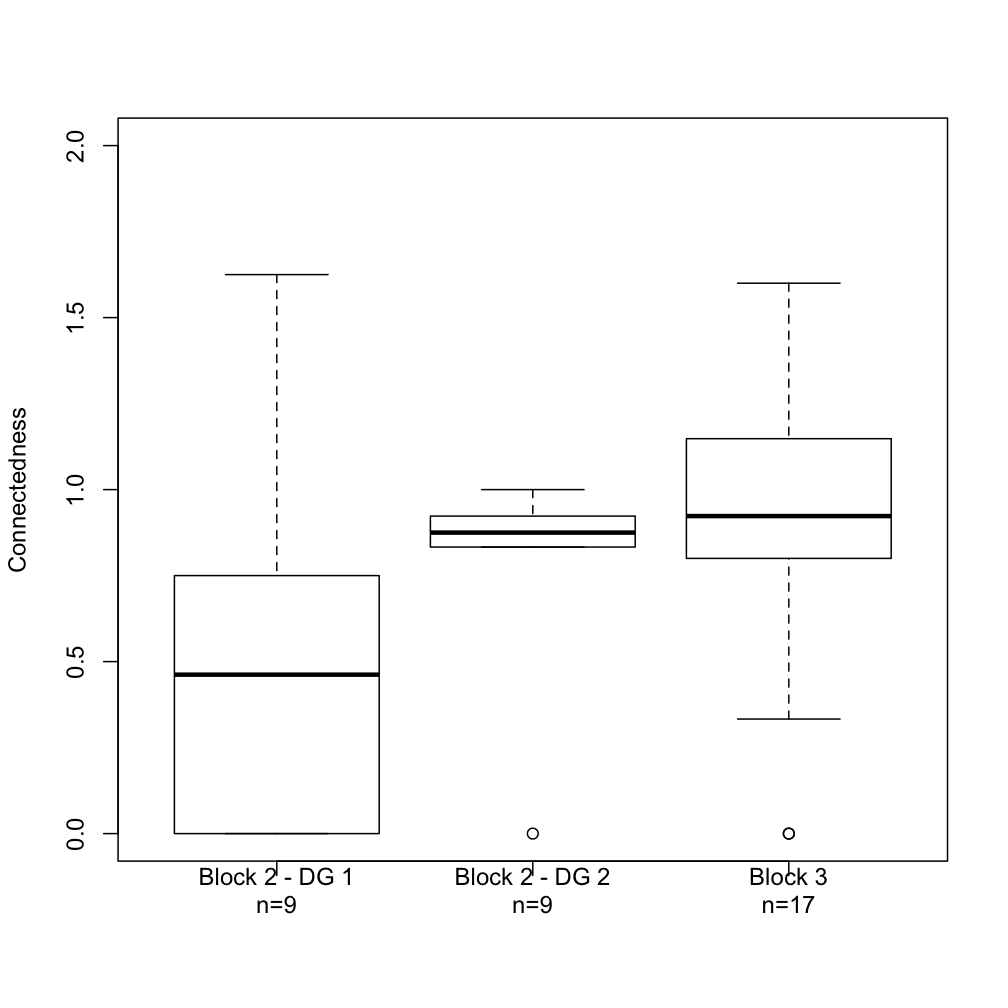
\includegraphics[height=3in]{img/Evaluierung/connectednessOverview.png}
	\caption{Connectedness in den Evaluierungsblöcken 2 und 3}
	\label{fig:img_Evaluierung_connectednessOverview}
\end{figure} 

Zu prüfen ist, ob die Connectedness in jenem Evaluierungs-Blöcken bzw. -Durchgängen, in denen die alternative Funktionalität zur Verbindungs-Herstellung verfügbar war, signifikant höher ist, als in jenen, in denen dies nicht der Fall war. Berechnet wird die Signifikanz zwischen den Ergebnissen der beiden Durchgänge von Block 2 ($conn_{2-1}$: $M=0.480, SD=0.544$ und $conn_{2-2}$: $M=0.804, SD=0.308$) sowie zwischen den Ergebnissen des ersten Durchgangs von Block 2 und den Ergebnissen von Block 3 ($conn_{3}$: $M=0.876, SD=0.435$). Im zweiten Fall ist zu beachten, dass die Aufgabenstellung nicht identisch war und diese Einfluss auf die Connectedness des Modells haben kann. Aufgrund der bestätigten Nicht-Normalverteilung der Stichprobe $conn_{2-2}$ (Sharpiro-Wilk-Test: $W_{2-1}=0.854, p_{2-1}=0.0823$, $W_{2-2}=0.586, p_{2-2}<0.005$, $W_{3}=0.913, p_{3}=0.114$) kommt zur Prüfung der Signifikanz der t-Test nicht in Frage, es wird der Wilcoxon-Test herangezogen.

Der einseitige Wilcoxon-Test für gepaarte Stichproben ergibt für $conn_{2-1}$ und $conn_{2-2}$ in der zweiten Stichprobe (jene mit Einsatz der alternativen Funktionalität der Verbindungsherstellung) eine signifikant höhere Connectedness ($V=5, p=0.0400$) als in der erste Stichprobe (ohne diese Funktionalität). 

Für $conn_{2-1}$ und $conn_{3}$ ergibt der einseitige Wilcoxon-Test für ungepaarte Stichproben ein ähnliches Ergebnis -- auch hier ist im der zweiten Stichprobe bei Einsatz der alternativen Funktionalität zur Verbiundungsherstellung eine signifikant höhere Connectedness festzustellen ($W=39, p=0.0227$).

Für $conn_{2-2}$ und $conn_{3}$ zeigt der zweiseitige Wilcoxon-Test für ungepaarte Stichproben dahingegen keine signifikant unterschiedliche Connectedness ($W=64.5, p=0.535$) für den zweitgenannten Block -- in diesem Fall kam in beiden Stichproben die alternative Möglichkeit zur Herstellung von Verbindungen zum Einsatz.

\subsubsection{Diskussion} % (fold)

Aufgrund der Ergebnisse der berechneten Signifikanztests ist die Hypothese anzunehmen. Mit der Einführung der alternativen Möglichkeit zur Herstellung von Verbindungen war in den einzelnen Anwendungen des Werkzeugs eine Zunahme der Verwendung von Verbindern zu beobachten. Während die Benutzer bei der ursprünglichen Funktion zur Herstellung von Verbindungen zum Großteil auf diese verzichteten (dieses Verhalten ist auch in Evaluierungsblock 1 zu beobachten), wurden Verbinder unabhängig von der Aufgabenstellung mit der Einführung der alternativen Funktionalität verstärkt eingesetzt.

Die Connectedness eignet sich als Parameter zur vergleichenden Beurteilung des Ausmaßes der Verwendung von Verbindern, da durch die Einbeziehung der Größe des Modells (repräsentiert durch die Anzahl der verwendeten Modellelemente) in die Berechnung den Wert für unterschiedliche Modelle vergleichbar gemacht wird. 

Einfluss auf die Höhe der Connectedness kann aber die Aufgabenstellung haben, die zur Bildung des Modells führt. Unterschiedliche Modellierungsaufgaben können zu unterschiedlichen Modell-Topologien führen, die sich wiederum in der Anzahl der verwendeten Verbinder auswirkt. Concept-Mapping-Aufgaben, die $conn_{3}$ zugrunde liegen, führen eher zu stärker verbundenen Modellen als Arbeitsabstimmungs-Aufgaben, auf denen $conn_{2-2}$ basiert und die zu eher ablauforientierten Modellen führen. Während bei Concept Mapping beliebige Konzepte in Beziehung stehen können, stehen Elemente bei ablauf-orientierten Modellen vor allem mit ihren kausalen Vorgängern und Nachfolgern in Beziehung, was die Anzahl der Verbinder einschränkt.

Dies ist am Ergebnis des Wilcoxon-Tests für $conn_{2-2}$ und $conn_{3}$ allerdings nicht zu erkennen -- in beiden Fällen stand die alternative Möglichkeit zur Verbindungsherstellung zur Verfügung. $conn_{3}$ unterscheidet sich nicht signifikant von $conn_{2-2}$. Die überarbeitete Möglichkeit zur Herstellung von Verbindern scheint die Auswirkung der unterschiedlichen Aufgabenstellung zu übertreffen bzw. zu kompensieren

Das Resultat der durgeführten Wilcoxon-Tests zwischen $conn_{2-1}$ und $conn_{2-2}$, $conn_{2-1}$ und $conn_{3}$ sowie $conn_{2-2}$ und $conn_{3}$ spricht für die Annahme der Hypothese \ref{hyp:verbinder}. Zu berücksichtigen ist hier jedoch die geringe Stichprobengröße, die die Aussagekraft des Ergebnisses schmälert.

\subsubsection{Ergebnis} % (fold)

Die Auswertung zeigt eine signifikant höhere Verwendung von Verbindern bei Verfügbarkeit der alternativen Funktionalität zur Verbindungs-Herstellung unabhängig von der Aufgabenstellung (siehe dazu auch die Diskussion von Hypothese \ref{hyp:keine_verbinder} in Abschnitt \ref{sub:abbildung_von_zusammenhängen_ohne_verbinder}). \textbf{Hypothese \ref{hyp:verbinder} kann auf Basis der vorliegenden Daten bestätigt werden.}

% subsection herstellung_von_verbindern (end)

\subsection{Verwendung des Löschtokens} % (fold)
\label{sub:verwendung_des_löschtokens}

In diesem Abschnitt werden die Ergebnisse der Überprüfung der Hypothese \ref{hyp:radierer} („Das Löschtoken ermöglicht intuitives Löschen von Modellelementen.“) vorgestellt. Die Auswertung basiert auf den Ergebnissen der Modellierungsblöcke 2, 3, 4 und 5, wobei zwischen Evaluierungsblöcken 3 und 4 die Funktionaliät und Verwendungsweise des Tokens überarbeitet wurde.

\subsubsection{Auswertung} % (fold)

Zur Auswertung wurde erhoben, in welchem Ausmaß das Löschtoken zum Entfernen unerwünschter Verbinder im Gegensatz zur alternativen Möglichkeit -- dem Einsatz der Wiederherstellungsfunktion -- verwendet wurde. Zusätzlich wurde erhoben, in wie vielen Fällen die Verwendung des Löschtokens scheiterte, weil die Benutzer dessen Einsatzmöglichkeit inkorrekt interpretierten. Tabelle \ref{tab:fehlinterpretationen} zeigt diese Daten für die Evaluierungsblöcke 2 bis 5.

\begin{table}[htbp]
	\centering
	\caption{Verwendung des Löschtokens}
\begin{tabular}{| c || c || c | c | c | c |}
  \hline
   EB    & Anw. & $L_{ges}$ & $L_{Token}$ & $FI_{Token}$ & $L_{WH}$ \\ \hline
   2     & 18 & 55 & 11 & 10 & 44 \\ 
   3     & 18 & 68 &  8 &  7 & 60 \\ 
   4     & 10 & 35 & 20 &  0 & 15 \\ 
   5     & 11 & 95 & 83 &  0 & 12 \\ \hline
   Ges.  & 57 & 253 & 122 & 17 & 131 \\ \hline
\end{tabular} \\
\footnotesize EB \ldots Evaluierungsblock, $L_{ges}$ \ldots Gesamtanzahl der Löschvorgänge, $L_{Token}$ \ldots Löschvorgänge mit Löschtoken, $FI_{Token}$ \ldots Fehlinterpretationen bei der Verwendung des Löschtokens, $L_{WH}$ \ldots Löschvorgänge mit Wiederherstellungsfunktion
	\label{tab:fehlinterpretationen}
\end{table}

Die Art der Fehlinterpretationen der Verwendung des Löschtokens kann durch nähere Betrachtung mittels der durchgeführten Interaktionsanalyse exakter bestimmt werden. Ausgewählt wurden hier Beispiele aus den Modellierungsblöcken 2 und 3. Die gesammelten Transkripte sind in den in Anhang \ref{cha:daten_der_empirischen_untersuchung} genannten Quellen verfügbar.

In der ersten hier angeführten Szene versuchen die Teilnehmer, die Beschriftung eines Blocks mit dem Löschtoken auszuradieren. Dies scheitert, da das Löschtoken als Zustandsschalter fungiert und das eigentliche Löschen separat ausgelöst werden muss. Außerdem wirkt das Löschtoken nur auf Verbindungen.

\begin{transkript}
	\emph{Die Teilnehmer möchten einen Block umbenennen.}\\
	\textbf{A:} Wie haben wir jetzt gesagt \emph{(markiert den roten Baustein)} keine Modellierungsvorgabe \emph{(gibt Bezeichnung ein)}\\
	\emph{System übernimmt die neue Beschriftung für den Baustein nicht.}\\
	\textbf{A:} Wo wurde das hingeschrieben? \emph{(Pause)} Radiergummi? Glaubst du, kann man das wegradieren?\\
	\textbf{B:} Probiere es aus.\\
	\textbf{\emph{A legt Radiergummi zum Block mit der Absicht die Beschriftung zu löschen}}\\
	\textbf{B:} Nein! Du löscht alles. Hör auf! \\
	\textbf{A:} Ok, wie war das zuerst? Lassen wir das mal weg. \emph{(legt Baustein zur Seite)}\\
	\emph{A legt den Block zur Seite.} 
\end{transkript}

Ein ähnliches Missverständnis zeigt sich auch in der im Folgenden angegebenen Situation. Hier sollte eine Verbindung gelöscht werden, das Löschtoken wurde jedoch wiederum nicht als Zustandsschalter, sondern für den Vorgang des Löschens selbst verwendet.

\begin{transkript}
	\emph{TLN A und B stellen jeweils ihren Marker zu den Blöcken, die verbunden werden sollen. Dabei wird eine gerichtete Verbindung erstellt.}\\
	\textbf{C:} Jetzt haben wir aber einen Pfeil gebastelt.\\
	\textbf{B:} Ja stimmt. Interessant.\\
	\textbf{A:} Wie war das mit dem Radiergummi? \emph{(nimmt Radiergummi und legt ihn auf die Verbindung)}\\
	\textbf{B:} Nein\\
	\textbf{C:} Nein, mit dem Glas! Du löscht alles!\\
	\textbf{A:} Nein, nur die Verbindung. \textbf{\emph{(Macht Radierbewegungen auf der Verbindung)}}\\
	\textbf{C:} Ich glaube, dass wir das Glas nehmen müssen.\\
	\emph{A schiebt die Blöcke, zwischen denen die Verbindung gelöscht werden soll, zusammen.}\\
	\textbf{A:} Da es funktioniert. \emph{(schiebt die Blöcke weiter auseinander und bemerkt, dass die Verbindung nicht gelöscht wurde)} Nein.\\
	\textbf{B:} \textbf{Ich glaube, der Radiergummi vernichtet alles.}\\
	\textbf{A:} Nein, der Radiergummi vernichtet nur Verbindungen. Nur welche? \emph{(schiebt beide Blöcke wieder zusammen – nimmt Radiergummi weg und schiebt Blöcke in die Ausgangsposition)}
\end{transkript}

In der folgenden Szene zeigen sich wiederum die Fehlinterpretationen der am Beginn angeführten Interaktion. Wieder wird das Token zum Radieren verwendet, Zielobjekt ist in diesem Fall die Beschriftung einer Verbindung.

\begin{transkript}
	\emph{Es wird eine falsche Beschriftung eingefügt. Die Teilnehmer wollen diese löschen, verwenden den Radiergummi allerdings falsch.}\\
	\textbf{B:} Aber irgendwie steht jetzt Ereignisse nicht bei dem Ding \emph{(zeigt auf gelben Block)}, sondern dort \emph{(zeigt auf beschriftete Verbindung)}.\\
	\emph{A verrückt den gelben Block ein wenig.}\\
	\textbf{B:} Normal ist das nicht, oder?\\
	\textbf{C:} Nein.\\
	\emph{A nimmt den Radiergummi.}\\
	\textbf{A:} Ich glaube das. \emph{(setzt den Radiergummi auf die Arbeitsfläche)}\\
	\textbf{C:} Aber nicht alles!\\
	\emph{A nimmt Radiergummi wieder weg. System erstellt eine Verbindung zwischen zwei roten Blöcken. Teilnehmer lachen. \textbf{A legt Radiergummi auf die erstellte Verbindung, und nimmt ihn wieder weg.} A nimmt die beiden verbundenen Blöcke und verschiebt sie.}\\
	\textbf{A:} Vielleicht so. \emph{(führt die Blöcke zusammen)}
\end{transkript}

In der folgenden Szene sind die Teilnehmer durch den Farbwechsel der Oberfläche beim Aufsetzen des Löschtokens (zur Indikation des Zustandswechsels) irritiert, da sie ebenfalls versuchen, das Token zum Radieren zu verwenden.

\begin{transkript}
	\emph{In der Szene erstellt das System einen ungewollten Verbinder, die Teilnehmer versuchen auf verschiedene Arten den Verbinder zu löschen.}\\
	\textbf{B:} Und wie kann ich die Verbindungen löschen?\\
	\textbf{B:} Warte einmal, da gibt es irgendwo das mit dem Radiergummi.\\
	\textbf{A:} murmelt zustimmend \\
	\emph{\textbf{B nimmt den Radiergummi und platziert ihn direkt auf dem Verbinder}}\\
	\emph{Das System färbt den Tisch rot}\\
	\textbf{A:} Nein, warte. Da löscht du alles!\\
	\emph{\textbf{B verschiebt den Radiergummi auf dem Tisch, hebt ihn an und platziert ihn direkt auf einem Block.}}\\
	\emph{Sobald der Radiergummi von der Oberfläche auf den Block gelegt wurde, entfernt das System die rote Färbung.}\\
	\textbf{A:} Ich glaube, da löscht du alles.\\
	\emph{B legt den Radiergummi an mehreren Stellen trotz der Warnung von TN A auf die Oberfläche}\\
	\textbf{B:} Nein, es will eh nicht.\\
\end{transkript}

Die nachstehende Interaktion zeigt wiederum die in den anderen Szenen bereits beschriebene Fehlinterpretation in der Verwendung des Löschtokens. Zusätzlich verwirrt eine Fehlfunktion des Werkzeugs, das anstelle eines Löschvorgangs einen Verbinder hinzufügt.

\begin{transkript}
	\emph{C versucht die Benennung eines Verbinders mittels Radiergummi zu entfernen.}\\
	\textbf{B:} Aber irgendwie steht jetzt Ereignisse nicht bei dem Ding \emph{(deutet auf einen Block)}, sondern dort \emph{(deutet auf einen Verbinder)}. Das wollen wir nicht oder?\\
	\textbf{A:} Nein.\\
	\textbf{C:} Ich glaube das. \emph{\textbf{(nimmt den Radiergummi und legt ihn auf den Verbinder, den die Teilnehmer entfernen wollen.)}}\\
	\textbf{A:} Aber nicht alles.\\
	\emph{C entfernt den Radiergummi wieder von der Modellierungsoberfläche. In diesem Moment erstellt das System durch Fehlerkennungen automatisch einen neuen Verbinder. C versucht, den neuen Verbinder mittels Radiergummi zu entfernen.}\\
	\textbf{A:} Oh Gott.\\
	\textbf{C:} Vielleicht so \emph{(schiebt die beiden betroffenen Blöcke zusammen)}, nein.\\
	\textbf{B:} Nein.\\
	\textbf{A:} Oh Gott, oh Gott, oh Gott.\\
	\textbf{B:} Gehen wir einen Prozessschritt zurück.\\
	\textbf{C:} Genau.\\
\end{transkript}

In der letzten hier angeführten Szene interagieren die Teilnehmer beinahe wie im Interaktionsdesign ursprünglich intendiert mit dem System. Sie scheitern letztendlich trotzdem und greifen zu alternativen Möglichkeit der Fehlerkorrektur, der Wiederherstellungsfunktion.

\begin{transkript}
	\emph{Teilnehmer versuchen mit dem Radiergummi und nur einem anderen Marker einen Verbinder zu entfernen.}\\
	\textbf{B:} Können wir die nicht so auch einfach löschen?\\
	\textbf{C:} Ja, mit dem Radiergummi.\\
	\textbf{B:} \textbf{Muss ich den jetzt zuerst so \emph{(Hält den Radiergummi zur Kamera)} hinhalten?}\\
	\textbf{A:} Nein, ich glaube, \textbf{den musst du einfach da \emph{(zeigt auf den Verbinder)} drauf legen.}\\
	\emph{B legt den Radiergummi auf den vom System automatisch erstellten Verbinder.}\\
	\textbf{A:} Und jetzt muss man \emph{(legt ein Markierungtoken auf den Verbinder)} Nein.\\
	\emph{Der Verbinder lässt sich auf diese Art nicht löschen und die Teilnehmer entscheiden sich, den Fehler mittels der Wiederherstellungsfunktion zu beseitigen.}
\end{transkript}

\subsubsection{Diskussion} % (fold)

In der quantitativen Auswertung ist klar zu erkennen, dass die ursprüngliche Implementierung der Löschfunktion, in der das Löschtoken als Zustandsumschalter fungierte, von den Benutzern kaum verwendet wurde und in jenen Fällen, in denen es zum Einsatz kam, falsch interpretiert wurde, was letztendlich zum Scheitern des Löschvorgangs führte. Beginnend mit Block 4 wurde die Löschfunktion in einer vollständig erneuerten Implementierung eingesetzt, in der das Löschtoken tatsächlich zum „Ausradieren“ einer Verbindung verwendet werden konnte. Damit wurde der vorherrschenden Interpretation der Funktionalität durch die Benutzer Rechnung getragen, was sich dadurch äußert, dass die Anzahl der Fehlinterpretationen auf 0 sank und das Löschtoken in weitaus höherem Ausmaß als die Wiederherstellungsfunktion zur Fehlerkorrektur verwendet wurde.

Bei der Betrachtung der Hypothese muss also zwischen der ursprünglichen Implementierung und deren neuen Umsetzung unterschieden werden. Für die ursprüngliche Implementierung kann die Hypothese nicht bestätigt werden, das Werkzeug war in der vorliegenden Form für die Benutzer nicht verständlich. In der Neuimplementierung wurden die ursprünglichen Fehlinterpretationen berücksichtigt und das Werkzeug so modifiziert, dass es entsprechend der beobachteten Benutzerinterpretation verwendet werden konnte. In dieser Variante sprechen die erhobenen Daten für eine Bestätigung der Hypothese.

\subsubsection{Ergebnis} % (fold)

\textbf{Hypothese \ref{hyp:radierer} muss für die ursprüngliche Umsetzung der Löschfunktion abgelehnt werden, kann aber für die neu konzipierte und implementierte Variante bestätigt werden.} In der ursprünglichen Umsetzung war die Verwendung des Werkzeugs für die Benutzer nicht verständlich, die eigentlich aufwändigere Alternativfunktion zur Fehlerkorrektur wurde außerdem weitaus häufiger verwendet. Nach der Neukonzeption kam es zu keinen Fehlinterpretationen mehr, das Löschtoken wurde außerdem in weitaus höherem Ausmaß verwendet.

% subsection verwendung_des_löschtokens (end)
% section ergebnisse (end)

\section{Zusammenfassung}
\label{sec:t_zusammenfassung}

In diesem Kapitel wurde die Evaluierung der Verwendbarkeit des Werkzeugs beschrieben. Die hier formulierten Hypothesen beschäftigen sich dementsprechend mit den grundlegenden Funktionen des Werkzeugs und den Interaktionsmöglichkeiten der Benutzer mit diesen. Nicht Gegenstand dieses Kapitels waren die im Kontext der Durchführung von „Articulation Work“ erstellten Modelle (siehe Kapitel \ref{cha:eval_aw}) sowie die Auswirkungen der Durchführung in der „Production Work“ (siehe Kapitel \ref{cha:eval_aw}).

In diesem Kapitel wurden sechs Hypothesen zur Werkzeugbenutzung getestet, die unmittelbar aus den Anforderungen an das Werkzeug (siehe \ref{cha:anforderungen}) abgeleitet waren. Zwei weitere Hypothesen zur Werkzeugverwendung wurden im Verlauf der ersten Evaluierungsblöcke explorativ gebildet und in den späteren Evaluierungsblöcken getestet. Die sechs aus den Anforderungen abgeleiteten Hypothesen bilden im Wesentlichen die Kernfunktionen des bzw. Interaktionsmöglichkeiten mit dem Werkzeug ab. Durch die Prüfung dieser Hypothesen wird so das gesamte Werkzeug einer Überprüfung hinsichtlich dessen praktischer Verwendbarkeit unterzogen.

Hypothese \ref{hyp:diagmodelle} („Repräsentation diagrammatischer Modelle“) bildet den grundlegenden Anspruch des Werkzeugs ab, die Abbildung von diagrammatischen Modellen zu ermöglichen. Diese werden als Repräsentation für externalisierte mentale Modelle verwendet und bilden so die Grundlage für die Durchführung von expliziter „Articulation Work“. Diese Hypothese konnte im Rahmen der Untersuchung bestätigt werden. Die Abbildung von Konzepten und Beziehungen zwischen diesen wurde in allen vorliegenden Modellen erfolgreich umgesetzt, wenngleich die Modellierung von expliziten Verbindungen in den ersten beiden Evaluierungsblöcken aufgrund von technischen Unzulänglichkeiten nicht durchgeführt wurde.

Hypothese \ref{hyp:kollaborativ} („Kooperatives Arbeiten“) prüft, ob die kooperative Verwendung des Werkzeugs möglich ist. Für die Durchführugn von „Articulation Work“ ist der kooperative Einsatz notwendig, da nur so die dabei ablaufenden synchronen Abstimmungsprozesse ermöglicht bzw. unterstützt werden können. Die Hypothese konnte in der Untersuchung bestätigt werden. Der Zeitanteil an der Modellbildung ist für Anwendungen mit zwei Teilnehmern weitgehend gleichverteilt, beide Teilnehmer beteiligen sich also an der Modellierung. Bei mehr als zwei Anwendern ist die Gleichverteilung nicht mehr gegeben, die Teilnehmer haben dennoch durchwegs (unabhängig von der Anzahl der Teilnehmer bei einer Anwendung) den Eindruck, sich einbringen zu können und gut zusammenarbeiten zu können.

Hypothese \ref{hyp:kontexte} („Einsetzbarkeit in unterschiedlichen Kontexten“) legt den Anspruch an das Werkzeug fest, dass dessen Anwendung unabhängig von der konkreten Anwendungsdomäne möglich ist. Wesentlich ist hierbei, dass das Werkzeug von Teilnehmer mit unterschiedlichen beruflichen bzw. Ausbildungs-Hintergründen gleich gut verwendet werden kann und dass die Modellbildung durch das Werkzeug nicht spezifisch für bestimmte Aufgabenstellungen erschwert wird. Die Hypothese konnte im Rahmen der Untersuchung bestätigt werden. Die Untersuchung der Korrelation zwischen Modellgröße und Modellierungsdauer zeigt unabhängig vom Anwendungskontext eine positive Korrelation, was darauf hinweist, dass der Aufwand zur Modellerstellung unabhängig von Aufgabenstellung und Anwendungskontext relativ stabil bleibt. Auch die Rückmeldungen der Teilnehmer mit unterschiedlichen beruflichen Hintergründen sind im Wesentlichen identisch, so dass das Werkzeug unabhängig vom Anwendungskontext immer ähnliche Wirkungen auf die Modellbildung zu haben scheint. 

Hypothese \ref{hyp:wiederherstellung} („Wiederherstellung vergangener Modellzustände“) prüft, ob die Bereitschaft zur Erstellung unterschiedlicher Modellvarianten im Verlauf der Modellbildung durch die Möglichkeit zur Wiederherstellung vergangener Modellzustände gefördert wird. Diese Hypothese kann auf Basis der Untersuchung nicht bestätigt werden. Die Wiederherstellungsfunktion wird nur in unter 10\% der untersuchten Anwendungen zur Verfolgung alternativer Modellierungswege genutzt. Die Funktion wird außerdem von den Anwendern bei der Frage nach den als nützlich wahrgenommene Funktionen in keinem der betrachten Fälle genannt, so dass davon ausgegangen werden muss, das sie nicht als relevant für die Durchführung der Modellbildung erachtet wird.

Hypothese \ref{hyp:behinderung} („Nicht-Behinderung“) geht auf die Gesamtwirkung des Werkzeugs bei der Modellbildung ein und untersucht, ob diese durch das Werkzeug behindert wird. Im Wesentlichen sind Bedienungsprobleme und technische Fehlfunktionen des Werkzeugs zu betrachten, die einen negativen Effekt auf die Ausführung der eigentlichen Aufgabe haben können. Die Hypothese konnte im Rahmen der Untersuchung nicht bestätigt werden. Bei der Benutzung des Werkzeugs traten vor allem in den ersten Evaluierungsblöcken Fehlfunktionen auf, die die Modellbildung massiv behinderten oder teilweise verhinderten. Durch Stabilisierung und Überarbeitung der technischen Plattform konnten diese Fehlfunktionen zwar minimiert werden, insgesamt können die Verbesserungen die gemessenen Werte nicht soweit verbessern, dass die Hypothese statistisch signifikant bestätigt werden könnte. Diese erhobenen Aspekte sind auch durch die überwiegend positive Benutzereinschätzung des Werkzeuges nicht als kompensiert anzusehen.

Hypothese \ref{hyp:gewöhnung} („Gewöhnung an das Werkzeug“) prüft, ob die wiederholte Verwendung des Werkzeugs dessen Bedienbarkeit durch die Benutzer verbessert. Betrachtet wurde hier einerseits die Modellierungsdauer im Verhältnis zur Modellgröße, was ein Maß für die Geschwindigkeit der Modellierung darstellt. Andererseits wurde die Anzahl der Fehlbedienungen des Werkzeugs betrachtet, die bei besserer Bedienbarkeit in wiederholten Anwendungen geringer ausfallen sollte. Die Hypothese kann auf Basis der vorliegenden Daten nur teilweise bestätigt werden. Während kein signifikanter Beschleunigungseffekt bei wiederholter Verwendung des Werkzeugs festgestellt werden konnte, war eine signifikante Verringerung der Anzahl der Fehlbedienungen des Werkzeugs bei wiederholtem Einsatz feststellbar.

Hypothese \ref{hyp:keine_verbinder} („Herstellung von Verbindern“) wurde explorativ aus Beobachtungen in den Evaluierungsblöcken 2 und 3 abgeleitet. In diesen Blöcken stieg die Verwendung von Verbindern im Modell sprunghaft an. Geprüft wurde nun, ob dies -- wie vermutet wurde -- auf die überarbeiteten und erweiterten Möglichkeiten zur Herstellung von Verbindern im Modell zurückzuführen war. Die Hypothese konnte in der Untersuchung bestätigt werden. Die Auswertung zeigt eine signifikant höhere Verwendung von Verbindern bei Verfügbarkeit der überarbeiteten Funktionalität zur Verbindungs-Herstellung. Allerdings scheint auch die Natur der Aufgabenstellung hohen Einfluss auf die Verwendung von Verbindern zu haben. Diese Vermutung wurde in Hypothese \ref{hyp:keine_verbinder} nochmals aufgegriffen und dort genauer untersucht (siehe dazu  Abschnitt \ref{sub:abbildung_von_zusammenhängen_ohne_verbinder}).

Hypothese \ref{hyp:radierer} („Verwendung des Löschtokens“) betrachtet ebenfalls eine Funktionalität des Werkzeugs, die auf Basis von Beobachtungen der Benutzerinteraktionen überarbeitet wurde. Die Funktion zur Entfernung von Verbindern wurde in den ersten Evaluierungblöcken kaum verwendet und zeigte im Falle der Verwendung hohes Potential für Missverständnisse hinsichtlich der Art der Benutzung. Die zur Verwendung notwendigen Interaktionsabläufe wurden daraufhin an die offensichtlich vorherrschende Interpretation der Benutzter, wie das entsprechende Werkzeug zu verwenden wäre, angepasst. Untersucht wurde nun, ob diese Anpassung die Entfernung von Elementen aus dem Modell erleicherte bzw. intuitiv gestaltete. Die Hypothese konnte für die überarbeitete Variante des Löschtokens bestätigt werden. In der ursprünglichen Umsetzung war die Verwendung des Werkzeugs für die Benutzer nicht verständlich, die eigentlich aufwändigere Alternativfunktion zur Fehlerkorrektur mittels der Wiederherstellungsfunktion wurde außerdem weitaus häufiger verwendet. Nach der Neukonzeption kam es zu keinen Fehlinterpretationen mehr, das Löschtoken wurde außerdem in weitaus höherem Ausmaß verwendet.

Insgesamt zeigt sich, dass das Werkzeug in der vorliegenden Form weitgehend verständlich zu sein scheint und als nützlich sowie zum Teil benutzbar wahrgenommen wird. Das Werkzeug erfüllt die Grundanforderungen hinsichtlich der Abbildbarkeit diagrammatischer Modelle und der Ermöglichung kooperativen Arbeitens. Die Einsetzbarkeit in beliebigen Kontexten scheint gegeben zu sein, wobei aufgrund von technischen Instabilitäten die Verwendbarkeit vor allem in den frühen Phasen der Evaluierung eingeschränkt war. Jene Hypothesen, die auf die Verwendung spezifischer Funktionalitäten eingehen, zeigen eine gute Verständlichkeit und hohes Ausmaß an Verwendung der Basisfunktionalitäten der Modellierung (etwa Platzierung und Benennung von Blöcken, Herstellung von Verbindern, Löschen von Verbindern), offenbaren aber Schwächen in der Verständlichkeit und Akzeptanz der komplexeren Funktionen, wie etwa der Wiederherstellungsunterstützung für gespeicherte Modellzustände. Zusammenfassend scheint das Werkzeug den grundlegenden Anforderungen also gerecht zu werden, bietet aber Raum für Verbesserungen hinsichtlich der Verwendung der komplexeren Funktionen und der technischen Stabilität. Im folgenden Kapitel wird nun auf die Verwendung des Werkzeugs zur kooperativen Abbildung von Modellen eingegangen. 

\subsection{Beitrag zur globalen Zielsetzung}

Dieses Kapitel stellt die Untersuchung der Verwendbarkeit des entwickelten Werkzeugs dar und trägt so hinsichtlich der in Kapitel \ref{cha:einführung} argumentieren und in Kapitel \ref{cha:anforderungen} näher ausgeführten zu untersuchenden Aspekte zur Beantwortung der Fragestellung \ref{tf:empirie} („Ermöglicht das Instrument die effektive Durchführung von expliziter Articulation Work?“) bei. Die Ergebnisse zeigen die erwartete Verwendbarkeit des Werkzeugs zur Unterstützung der entwickelten Methodik und bestätigen so die grundlegende Voraussetzung für die effektive Unterstützung expliziter „Articulation Work“ durch das hier vorgestellte Instrument.

\subsection{Weitere Verwendung der Ergebnisse}

Die Ergebnisse dieses Kapitels werden in ihrer Gesamtheit erst in den Schlussbetrachtungen (Kapitel \ref{cha:schlussbetrachtungen}) wieder aufgegriffen. Einzelne Hypothesen, vor allem jene, die sich mit der kooperativen Verwendbarkeit des Werkzeugs beschäftigen, werden aber bereits in den folgenden beiden Kapiteln wieder aufgegriffen und dienen dort als Grundlage der Evaluierung der Methodik bzw. der Wirkung der durchgeführten „Articulation Work“.


% chapter eval_tui (end) 
% final draft
% todo: Interkapitel-Referenzen, Kontextgrafik, Qualitiative Fragebogen-Daten für Hypothese Kooperation


\chapter{Evaluierung der erstellten Modelle} % (fold)
\label{cha:eval_modell}

Im zweiten Teil der Evaluierung wird nicht der Umgang mit dem Werkzeug betrachtet (siehe dazu Kapitel \ref{cha:eval_werkzeug}), sondern auf das unmittelbare Resultat der Werkzeugverwendung, also das erstellte Modell eingegangen. Ebenfalls nicht Gegenstand der Untersuchung ist in diesem Abschnitt die Wirkung der Modellbildung auf die operative Arbeit („Production Work“), die in Kapitel \ref{cha:eval_aw} betrachtet wird. Abbildung \ref{fig:img_Kontextgrafiken_k13} stellt dieses Kapitel und dessen Aufbau im Kontext der anderen inhaltlich vor- und nachgelagerten Kapitel dar.


\begin{figure}[htbp]
	\centering
		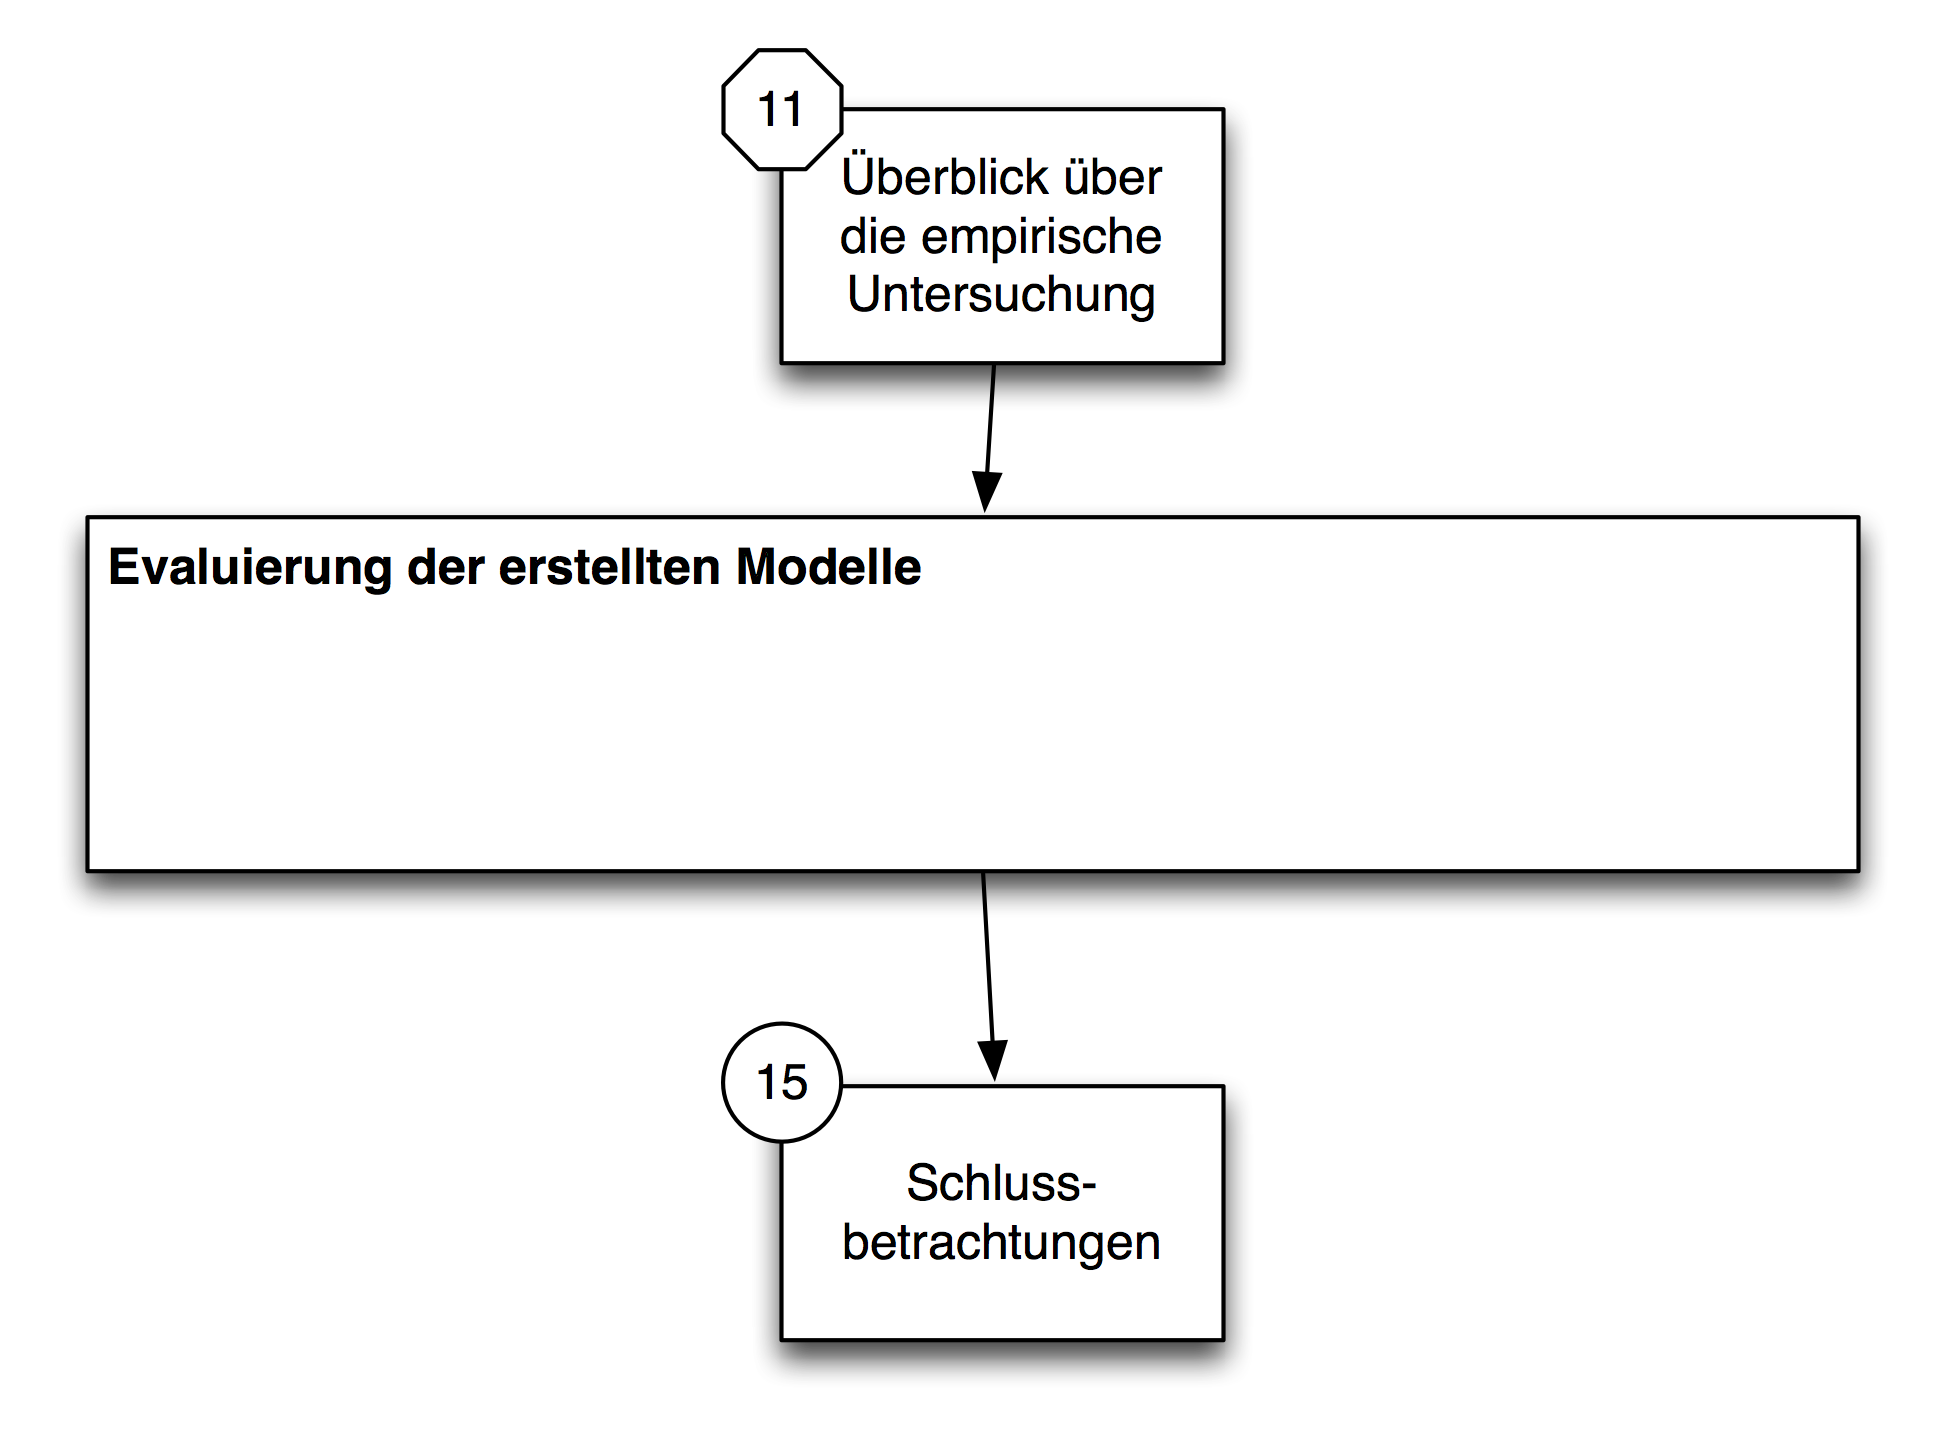
\includegraphics[scale=0.75]{img/Kontextgrafiken/k13.png}
	\caption{Kapitel „Evaluierung der erstellten Modelle“ im Gesamtzusammenhang}
	\label{fig:img_Kontextgrafiken_k13}
\end{figure}


Ausgehend von den erstellten Modellen und deren Entstehungsprozess wird also in diesem Kapitel untersucht, wie das Werkzeug auf die in dieser Arbeit gewählte Form der Unterstützung expliziter „Articulation Work“, nämliche der kooperativen Externalisierung und Abstimmung mentaler Modelle, wirkt. Dementsprechend sind die im folgenden Abschnitt beschrieben Hypothesen aus den Ausführungen der Kapitel über mentale Modelle (Kapitel \ref{cha:mentale_modelle}) und der Methodik zur Externalisierung derselben (Kapitel \ref{cha:methodik}) abgeleitet. 

Zusätzlich wird eine explorativ gebildete Hypothese untersucht, die sich auf inhaltlicher Ebene mit dem Phänomen der Abbildung von Zusammenhängen durch räumliche Konfiguration der Konzepte in einem Modell beschäftigt, das in der Untersuchung der Hypothese \ref{hyp:diagmodelle} bereits hinsichtlich der Werkzeugverwendung beschrieben wurde.

\section{Hypothesen} % (fold)
\label{sec:m_hypothesen}

In diesem Abschnitt werden die Hypothesen abgeleitet, die in diesem Kapitel geprüft werden. Wie in Kapitel \ref{cha:eval_werkzeug} ist zwischen konzeptuell aus der Aufgabenstellung bzw. der entwickelten Methodik abgeleiteten Hypothesen über die Wirkung des Werkzeugs und explorativ während der Evaluierung selbst gebildeten Hypothesen über Eigenschaften des Werkzeugs bzw. dessen Verwendung im Kontext der Modellbildung zu unterscheiden.

\subsection{Konzeptuell begründete Hypothesen} % (fold)
\label{sub:m_konzeptionell_begründete_hypothesen}

Die folgenden Hypothesen sind aus der Aufgabenstellung bzw. den Ausführungen zur Modellierungs-Methodik abgeleitet. Auf die entsprechenden Ausführungen in den Kapiteln \ref{cha:mentale_modelle} bzw. \ref{cha:methodik} wird jeweils bei der Begründung der Hypothesen verwiesen.

Ein wesentlicher Aspekt bei der Externalisierung mentaler Modelle ist die Offenheit der Repräsentationssprache. Diese ist aus Abschnitt \ref{sub:concept_mapping} begründbar und in Anforderung \ref{anf:nicht_vorgegebene_semantik_der_modellierungselemente} abgebildet. Unter „Offenheit“ ist in diesem Zusammenhang die Eigenschaft der Repräsentationssprache gemeint, keine vordefinierte Semantik der Modellelemente vorzugeben sondern diese von den Modellierenden festlegen zu lassen. Dies umfasst im vorliegenden Fall sowohl die Bedeutung der unterschiedlichen Konzepttypen als auch die Bedeutung der Verbindungen zwischen Konzepten. Das Werkzeug darf also in diesem Zusammenhang die Benutzer nicht bei der Wahl der Repräsentationskonzepte und damit bei der Externalisierung selbst einschränken. Die Prüfung dieser Hypothese ermöglicht die Beurteilung der Erfüllung der Anforderung \ref{anf:nicht_vorgegebene_semantik_der_modellierungselemente} (siehe Seite \pageref{anf:nicht_vorgegebene_semantik_der_modellierungselemente}).

\begin{hyp}
	\label{hyp:keine_einschränkung}
	Das Werkzeug schränkt Benutzer semantisch nicht bei der Externalisierung ihrer mentalen Modelle ein.
\end{hyp}

Das Argument der Nicht-Beschränkung der Benutzer bei der Externalisierung hat neben der eben beschriebenen Sprach-Dimension auch eine konkrete Modell-Dimension. Während sich obige Hypothese auf semantische Einschränkungen der Externalisieungsmöglichkeiten bezieht, ist sind auch konkrete, strukturelle Einschränkungen bei der Verwendung des Werkzeugs zur Externalisierung eines bestimmten mentalen Modells zu berücksichtigten. Die Externalisierung muss -- um nicht beschränkend zu wirken -- beliebig umfangreiche Modelle ermöglichen. „Umfangreich“ bedeutet hier, dass das Modell beliebig viele Elemente enthalten können muss und diese beliebig untereinander in Beziehung gesetzt werden können. Die Prüfung dieser Hypothese ermöglicht die Beurteilung der Erfüllung der Anforderung \ref{anf:bearbeitung_von_beliebig_komplexen_modellen} (siehe Seite \pageref{anf:bearbeitung_von_beliebig_komplexen_modellen}).
	
\begin{hyp}
	\label{hyp:beliebige_komplexität}
	Das Werkzeug ermöglicht die Repräsentation beliebig umfangreicher Modelle.
\end{hyp}

Die Möglichkeit durch die Entstehungsgeschichte des erstellten Modells zu navigieren ist eine Funktion, die ebenfalls hinsichtlich ihrer Wirkung auf die Externalisierung mentaler Modelle untersucht werden muss. In der dieser Funktionalität zugrundeliegenden Literatur (\citep{Shipman00}, \citep{Klemmer02}) wird diese als wesentlich bezeichnet, wenn Externalisierungsprozesse unterbrochen werden, kollaborativ durchgeführt werden oder Dritten die Möglichkeit gegeben werden soll, die Entstehung des Modells nachzuvollziehen. Allen drei Aspekten liegt die Annahme zugrunde, dass in der Historie des Externalisierungsprozesses die dem Ergebnis zugrundeliegenden Ideen und Annahmen zu erkennen sind. Im Kontext dieser Arbeit bedeutet dies, dass aus der Nachverfolgung der Historie des externalisierten Modells die diesem zugrundeliegenden mentalen Modelle verständlich und nachvollziehbar werden. Die Prüfung dieser Hypothese ermöglicht die Beurteilung der Erfüllung der Anforderung \ref{anf:persistente_ablage_des_modells_möglichkeit_zur_rekonstruktion} (siehe Seite \pageref{anf:persistente_ablage_des_modells_möglichkeit_zur_rekonstruktion}).

\begin{hyp}
	\label{hyp:historie}
	Die Reflexion des Modellierungsverlaufs ermöglicht das Verständnis der dem Modell zugrundeliegenden mentalen Modelle.
\end{hyp}

Die Externalisierung mentaler Modelle mit Hilfe von computer-gestützten Werkzeugen ist keine originäre Idee dieser Arbeit. Computerunterstützung existiert vor allem im Bereich des „Concept Mapping“ (siehe Abschnitt \ref{sub:concept_mapping}), das methodisch maßgeblich in das vorgeschlagene Vorgehen des hier vorgestellten Ansatzes einfließt (siehe Kapitel \ref{cha:methodik}). In den existierenden Werkzeugen werden jedoch die kooperative Erstellung und kommunikative Validierung der externalisierten Modelle nicht explizit berücksichtigt. Beide Aspekte sind jedoch -- wie bei der Beschreibung der Strukturlegetechniken \ref{sub:strukturlegetechniken} ausgeführt -- wichtig für den Abgleich mentaler Modelle und damit für die erfolgreiche Durchführung von „Articulation Work“. Die Ermöglichung und Stärkung der Kooperation der Beteiligten untereinander ist also ein wesentlicher Teilaspekt der Anforderung \ref{anf:kollaborative_und_unmittelbare_manipulierbarkeit_des_modells} an das Werkzeug („Kooperative und unmittelbare Manipulierbarkeit des Modells“). Die Prüfung dieser Hypothese ermöglicht die Beurteilung der Erfüllung der Anforderung \ref{anf:kollaborative_und_unmittelbare_manipulierbarkeit_des_modells} (siehe Seite \pageref{anf:kollaborative_und_unmittelbare_manipulierbarkeit_des_modells}).

\begin{hyp}
	\label{hyp:stärkere_kooperation}
	Die Verwendung des Werkzeugs führt zu stärkerer Kooperation bei der Modellerstellung als die Verwendung von bildschirm-basierten Werkzeugen.
\end{hyp}

Hinsichtlich der in Kapitel \ref{cha:anforderungen} formulierten Anforderungen können die hier formulierten Hypothesen zusammenfassend wie folgt eingeordnet werden:

\begin{center}
\begin{tabular}{|c|c|}
  \hline
   Hypothese & Anforderung \\ \hline
   \ref{hyp:keine_einschränkung} & \ref{anf:nicht_vorgegebene_semantik_der_modellierungselemente} \\
   \ref{hyp:beliebige_komplexität} & \ref{anf:bearbeitung_von_beliebig_komplexen_modellen} \\
   \ref{hyp:historie} & \ref{anf:persistente_ablage_des_modells_möglichkeit_zur_rekonstruktion} \\
   \ref{hyp:stärkere_kooperation} & \ref{anf:kollaborative_und_unmittelbare_manipulierbarkeit_des_modells} \\ \hline
\end{tabular} 
\end{center}

% subsection konzeptionell_begründete_hypothesen (end)

\subsection{Explorativ gebildete Hypothesen} % (fold)
\label{sub:m_explorativ_gebildete_hypothesen}

Im Verlauf der beiden Evaluationen war die Herstellung von Verbindungen zwischen Modellelementen aus technischen Gründen schwierig zu benutzen und sehr anfällig für Fehlfunktionen. Dies führte dazu, dass Verbinder nahezu nicht verwendet wurden (siehe dazu die Auswertungen zu Hypothese \ref{hyp:diagmodelle} in Abschnitt \ref{sub:repräsentation_diagrammatischer_modelle}). In dieser Situation wurden Beziehungen zwischen Modellelementen von den Benutzern durch die räumliche Anordnung der Elemente ausgedrückt. Diese implizite Darstellung von relationaler Information erfolgte in allen Fällen spontan und ohne Anleitung oder Instruktion. Dies führte zu der Vermutung, dass die Verwendung von Verbindern zur Abbildung von Beziehungen bzw. Zusammenhängen zwischen Elementen nicht notwendig ist. Um diese Vermutung zu prüfen, wurde sie formal als Hypothese \ref{hyp:keine_verbinder} in die Untersuchung aufgenommen.

\begin{hyp}
	\label{hyp:keine_verbinder}
	Zur Abbildung von Zusammenhängen ist die Verwendung von Verbindern nicht notwendig.
\end{hyp}

% subsection explorativ_gebildete_hypothesen (end)

% section hypothesen (end)

\section{Untersuchungsdesign und Durchführung} % (fold)
\label{sec:m_untersuchungsdesign}

In diesem Abschnitt wird auf Basis der oben formulierten Hypothesen das Untersuchungsdesign abgeleitet und die Durchführung der Untersuchung beschrieben. Der erste Teil des Abschnitts beschreibt die Operationalisierung der Hypothesen und damit die Festlegung wie diese konkret geprüft werden können. Im zweiten Teil des Abschnitts wird die Durchführung der Prüfung beschrieben. Hier erfolgt neben der Zuordnung der einzelnen Evaluierungsblöcke (siehe Abschnitt \ref{sec:globales_untersuchungsdesign}) auch die Darstellung rein beschreibender Modell-Parameter, die nicht unmittelbar in die Prüfung der Hypothesen eingehen. 

\subsection{Operationalisierung} % (fold)
\label{sub:m_operationalisierung}

In diesem Abschnitt wird für jede Hypothese identifiziert, in welcher Form sie geprüft werden kann. Dies umfasst die Festlegung der Messpunkte sowie der jeweiligen Mess- und Auswertungsmethode (letzte bezugnehmend auf den in Abschnitt \ref{sec:eingesetzte_werkzeuge_und_verfahren} beschriebenen Verfahren). Zudem werden jene Evaluationsblöcke festgelegt, die für die jeweilige Untersuchung herangezogen wurden.

Für jede Hypothese wird also spezifiziert, anhand welcher Aspekte diese geprüft werden kann (= abhängige Variablen). Zudem wird festgelegt welche Ausgangssituation bei der Anwendung gewählt werden muss, um die Prüfung durchführen zu können (= unabhängige Variable) und welche Faktoren die Beurteilung ggf. ungewollt beeinflussen können (= Störvariablen).

\subsubsection{Keine semantische Einschränkung der Externalisierung} % (fold)
\label{ssub:keine_semantische_einschränkung_der_externalisierung}

Gegenstand dieses Abschnitts ist die Prüfung der Hypothese \ref{hyp:keine_einschränkung}. Diese bezieht sich auf die geforderte Eigenschaft des Werkzeugs, die Benutzer bei der Modellierung semantisch nicht einzuschränken.

Voraussetzung für die Prüfung dieser Hypothese ist die Verwendung des Werkzeugs zur Modellbildung bei einer Aufgabe, die die semantischen Kategorien der Strukturierung nicht vorgibt. In der eingesetzten Methodik wird die Festlegung von Elementtypen explizit gefordert (Vorgehen und Zeitpunkt dafür werden jedoch nicht vorgegeben). Etwaige Modellierungsvorkenntnisse können diese Festlegung insofern beeinflussen, als dass die Konzepte bekannter Sprachen bevorzugt eingesetzt werden könnten. Im Sinne der Hypothese ist dies jedoch keine Störvariable, da die Forderung nach nicht einschränkender Struktur auch die Verwendung existierender Modellierungssprachen umfassen muss.

Die nicht einschränkende Wirkung kann qualitativ anhand von Benutzeraussagen und dem Prozess und Ergebnis der Modellentstehung beurteilt werden. Im ersten Fall bieten sich neben der direkten Frage nach der Abbildbarkeit der gewünschten Information auch Teilaspekte des \gls{PMS}-Framework \citep{Sedera02} an, das unter anderem die subjektiv wahrgenommene Qualität des Modellierungsergebnisses und die Abbildbarkeit der subjektiv wichtigen Information im Modell abbildet (zur Eignung des \gls{PMS}-Frameworks im Kontext dieser Arbeit siehe \citep{Wahlmuller10}). Am Prozess- und Ergebnis der Modellentstehung selbst kann beurteilt werden, ob und inwieweit die zur Verfügung gestellten, semantisch nicht vorbelegten Modellierungselemente für die Abbildung der gewünschten Information ausreichend bzw. geeignet waren. Dazu kann betrachtet werden, ob die beschränkte Anzahl von Elementen im Verlauf der Modellierung zu verändertem Vorgehen in der Abbildung oder zur Nichtabbildung bestimmter Modellaspekte führte und ob durch semantische Mehrfachbelegung bzw. die Einführung von nicht als Modellierungselement vorgesehenen Bausteinen der Sprachumfang über das ursprünglich intendierte Maß hinaus erweitert wurde. 

Vergleichend können zusätzlich Modelle herangezogen werden, die aus identischen Fragestellungen wie jene mit dem Werkzeug erstellten resultieren, bei denen jedoch ein in der Anzahl und Semantik der Modellierungselemente frei erweiterbares Werkzeug zum Einsatz kommt. Hier ist von Interesse, ob die erstellten Modelle semantisch vielfältiger sind als jene, die mit dem hier vorgestellten Werkzeug erstellt wurden.

% subsubsection keine_semantische_einschränkung_der_externalisierung (end)

\subsubsection{Repräsentation beliebig umfangreicher Modelle} % (fold)
\label{ssub:repräsentation_beliebig_komplexer_modelle}

Gegenstand dieses Abschnitts ist die Operationalisierung der Hypothese \ref{hyp:beliebige_komplexität}. Dabei wird überprüft, ob das Werkzeug die Abbildung beliebig umfangreicher Modellierungsaufgaben ermöglicht.

Voraussetzung zur Prüfung dieser Hypothese ist die Verwendung von Modellierungsaufgaben, die zu umfangreichen Modellen führen. Umfangreichen Modellierungsaufgaben sind Aufgaben, die bei detaillierter Modellierung >15 Modellelemente benötigen\footnote{15 wurde als Grenze gewählt, weil diese Anzahl die Obergrenze an gleichzeitig am Werkzeug verwendbaren Elementen darstellt}). Dies ist deshalb notwendig, weil der wesentliche beschränkende Faktor des Umfangs eines Modells am hier vorgestellten Werkzeug die physisch eingeschränkte Größe der Modellierungsoberfläche ist. Etwaige Modellierungsvorkenntnisse der Benutzer sind bei der Prüfung dieser Hypothese nicht von Relevanz.

Um Schlussfolgerungen auf eine etwaig einschränkende Wirkung des Werkzeugs auf den Umfang der Modelle treffen zu können, muss eine entsprechende Aufgabenstellung einerseits mittels dem hier vorgestellten Werkzeug („Experimentalgruppe“) und andererseits mit einem Werkzeug, dass den Umfang der Modellierungsoberfläche nicht begrenzt („Kontrollgruppe“), abgebildet werden. Die Ergebnisse der beiden Gruppen werden dann gegenübergestellt. Falls bei identischer Fragestellung der Umfang der Modelle in der Kontrollgruppe signifikant höher ist als jener der Experimentalgruppe, kann von einer einschränkenden Wirkung ausgegangen werden und die Hypothese müsste abgelehnt werden.

Daneben sind wiederum Aussagen der Benutzer über die Abbildbarkeit umfangreicher Modelle zur Prüfung der Hypothese heranzuziehen. Entsprechende Fragen wurden in den Evaluierungsblöcken 2, 3, 4 und 5 gestellt, wobei die Fragestellungen in den Blöcken 2 und teilweise 4 eher zu nicht umfangreichen Modellen führte, die auf der Oberfläche ausreichend Platz fanden und deshalb hier nicht berücksichtigt werden können.

% subsubsection repräsentation_beliebig_komplexer_modelle (end)

\subsubsection{Reflexion des Modellierungsverlaufs} % (fold)
\label{ssub:reflexion_des_modellierungsverlaufs}

Gegenstand dieses Abschnitts ist die Operationalisierung der Hypothese \ref{hyp:historie}. Dabei wird überprüft, ob die Möglichkeit zur Reflexion des Modellierungsverlaufs das Verständnis der zugrundeliegenen mentalen Modelle ermöglicht bzw. verbessert.

Zur Prüfung dieser Hypothese müssen Modellierungsaufgaben durchgeführt werden, in deren Rahmen die Interpretation eines Modells durch an der Modellbildung nicht beteiligte Personen durchgeführt werden. Wenn diese Interpretation den ursprünglich vom Modellierer repräsentierten Inhalten entspricht, ist die Interpretation als erfolgreich zu bezeichnen. Zu beurteilen ist nun, in wie weit die Möglichkeit zur Wiedergabe des Modellierungsverlaufs bei der Interpretation genutzt wurde und ob diese Nutzung Auswirkungen auf die Interpretation hatte.

Zur Beurteilung wird eine Modellierungssituation geschaffen, in der eine Person für sich individuell das Werkzeug zur Externalisierung eines mentalen Modells benutzt. In einem zweiten Schritt wird eine zweite, zuvor nicht beteiligte Person aufgefordert, den Inhalt der auf der Modellierungsoberfläche vorhandenen Repräsentation zu interpretieren, wobei der Modellierungsverlauf herangezogen werden darf, eine Interaktion mit dem ursprünglichen Modellierer jedoch nicht gestattet ist. Im dritten Schritt beurteilt der ursprüngliche Modellierer die Adäquatheit der Interpretation und trifft so eine Aussage über den Erfolg des Transfers des mentalen Modells. In Kombination lässt sich eine qualitative Aussage über die Effekte der Wiederherstellungsfunktion treffen.    

% subsubsection reflexion_des_modellierungsverlaufs (end)

\subsubsection{Wirkung auf die Kooperation bei der Modellerstellung} % (fold)
\label{ssub:wirkung_auf_die_kooperation_bei_der_modellerstellung}

Gegenstand dieses Abschnitts ist die Operationalisierung der Hypothese \ref{hyp:stärkere_kooperation}. Gegenstand der Untersuchung ist hier, ob die Verwendung des Werkzeugs bei der Modellbildung zu stärkerer Kooperation zwischen den Beteiligten führt als der Einsatz von bildschirmbasierten Werkzeugen.

Die Prüfung der Wirkung des Werkzeugs auf die kooperative Abbildung von Modellen bedingt Fragestellungen, die Kooperation explizit einfordern. Etwaige Modellierungsvorkenntnisse beeinflussen die Prüfung der Hypothese nicht. Bei der Beurteilung zu berücksichtigen sind etwaige bestehende persönliche Bekanntschaften oder etablierte Gruppen, deren Zusammenarbeit bereits institutionalisiert ist. Um den Einfluss derartiger Faktoren möglichst auszuschließen, müssen die Gruppen bei der Modellbildung zufällig gebildet werden und etwaige Bekanntschaften innerhalb der gebildeten Gruppen explizit im Vorfeld der Untersuchung erhoben werden.

Die hier zu prüfende Hypothese baut auf Hypothese \ref{hyp:kollaborativ} auf. Dort war zu prüfen, ob das Werkzeug kooperatives Arbeiten grundsätzlich ermöglicht. In diesem Abschnitt wird geprüft, ob der Einsatz des Werkzeugs hinsichtlich der Kooperation der Beteiligten tatsächlich einen meßbaren Vorteil gegenüber einem traditionellen, bildschirmbasierten Werkzeug hat. Dazu ist es notwendig, eine vergleichende Untersuchung durchzuführen. Evaluierungsblock 5 wurde dementspechend geplant und umfasste eine die kooperative Abbildung eines Modells sowohl am Modellierungstisch als auch mittels dem bildschirmbasierten Werkzeug CMapTools. Die Aufgabenstellung wurde so gewählt, dass das resultierende Modell grundsätzlich in beiden Werkzeugen abgebildet werden konnte. Untersucht wurde, in welchem Ausmaß Kooperation zwischen den beteiligten Personen auftrat. Als Metriken dienten dazu die Zeitverteilung der Beteiligung am Modellierungsvorgang, der Zeitanteil an Diskussion während der Modellbildung sowie die Anzahl der Initiativwechsel („Turn-Taking“) während eines Durchgangs. Zusätzlich können die Benutzer hinsichtlich des subjektiv empfundenen Ausmaßes der Kooperation sowie der Zufriedenheit mit den im Modell sichtbaren von ihnen selbst eingebrachten Inhalten befragt werden.

Zur Berechnung der Zeitverteilung wird nicht der Zeitanteil der physischen, sondern jener der inhaltlichen Initiative herangezogen. Wo kein die Initiative führender Teilnehmer identifizierbar ist, wird der betreffende Zeitabschnitt zu gleichen Teilen zwischen den Teilnehmern aufgeteilt. Die Zeitverteilung zwischen den Teilnehmern kann dann insofern in die Prüfung einfließen, als dass sehr niedrige oder sehr hohe Zeit-Anteile auf eine unausgewogene Modellierungsbeteiligung hinweisen. Dieses Indiz muss jedoch durch Benutzeraussagen verifiziert werden, da geringe Beteiligung an der Modellierung nicht notwendigerweise auf als mangelhaft empfundene Kooperation hinweist.

Der Zeitanteil an Diskussion während des Modellierungsvorgangs betrifft tatsächlich nur jenen Anteil an der Modellierungsdauer, in dem ein inhaltlicher Austausch zwischen den Teilnehmern im Sinne der Aufgabenstellung stattfindet. Nicht berücksichtigt werden jene Zeiten, in denen das Modell erstellt wird oder in denen nicht im Sinne der Aufgabenstellung gearbeitet wird (etwa bei Fehlfunktionen).

Der Wechsel der Initiative („Turn-Taking“ \citep{Sacks74}) bei der Modellierung bezieht sich im Gegensatz zu der Berechnung der Zeitverteilung zwischen den Teilnehmern auf die physische Initiative bei der Erstellung des Modells. Während in der von \citet{Sacks74} vorgeschlagenen Methodik zur Identifikation von Initiativwechsel auf Konversationen eingegangen wird und damit auf Sprecherwechsel Bezug genommen wird, wird in diesem Fall die Übernahme der physischen Initiative als „Turn“ bezeichnet. Dies erscheint insofern sinnvoll, als das jener Teilnehmer, der die physische Kontrolle über die Eingabemedien besitzt auch exklusiven Zugriff auf die Interaktionsmöglichkeiten mit dem System besitzt und damit potentiell als „Filter“ zwischen den Eingaben der anderen Teilnehmer und der im System repräsentierten Information wirkt.

% subsubsection wirkung_auf_die_kooperation_bei_der_modellerstellung (end)

\subsubsection{Abbildung von Zusammenhängen ohne Verbinder} % (fold)
\label{ssub:abbildung_von_zusammenhängen_ohne_verbinder}

Gegenstand dieses Abschnitts ist die Operationalisierung der Hypothese \ref{hyp:keine_verbinder}. Gegenstand der Untersuchung ist die Beobachtung, dass zur Abbildung von Zusammenhängen die Verwendung von explizit dargestellten Verbindern nicht notwendig ist.

Die Prüfung dieser Hypothese stellt keine Vorbedingungen an die Modellierungsaufgabe oder die Modellierungsvorkenntnisse der Benutzer. Auch können individuelle Anwendungen der Werkzeugs (d.h. nicht nur in kooperativen Szenarien) zur Untersuchung verwendet werden. 

Bei der Prüfung der Hypothese sind zwei Formen der Notwendigkeit von explizit dargestellten Verbindern zu unterscheiden. Zum Einen ist die Notwendigkeit bei der kooperativen Erstellung eines Modells zu untersuchen, bei der sämtliche Beteiligte zu einer einheitlichen Interpretation des dargestellten Modells kommen sollen. Zum Anderen muss auch der Fall einer zeitlich nachgelagerten Interpretation durch Dritte untersucht werden. Hier ist zu erheben, ob die Interpretation der Modellinhalts dem ursprünglichen Verständnis des bzw. der Modellierenden entspricht.

Zur Untersuchung muss dem ursprünglichen Modellierer jeweils eine inhaltliche Interpretation des Modellierungsergebnisses rückgespiegelt werden. Diese Form der kommunikativen Validierung kommt methodisch im Rahmen der Anwendung von Strukturlegetechniken (siehe Abschnitt \ref{sub:strukturlegetechniken}) zum Einsatz und ist deshalb ohnehin Teil der in dieser Arbeit vorgeschlagenen Methodik bei der kooperativen Anwendung des Werkzeugs. Zur zeitlich nachgelagerten Interpretation bedarf es einem separaten Schritt, in dem das Modellierungsergebnis von einer dritten, den der Modellierung nicht beteiligten Person interpretiert und rückgespiegelt wird. 

% subsubsection abbildung_von_zusammenhängen_ohne_verbinder (end)
% subsection m_operationalisierung (end)

\subsection{Durchführung} % (fold)
\label{sub:m_durchführung}

In diesem Abschnitt werden die für diesen Evaluierungs-Teil relevanten deskriptiven Parameter der berücksichtigten Anwendungs-Blöcke angeführt.
Als Grundlage der Überprüfung der Hypothesen werden hier die Evaluierungs-Blöcke 1 bis 5 verwendet. Dabei wurden für die quantitativ zu prüfenden Variablen die Blöcke 2, 3 und 5 herangezogen, da in diesen die größten Stichproben zur Verfügung standen. In die qualitative Auswertung der Ergebnisse wurden hingegen alle Blöcke (1-5) mit einbezogen.

\subsubsection{Stichprobe} % (fold)
\label{ssub:stichprobe}

\begin{tabular}{| p{2cm} || p{2cm} | p{2cm} | p{2cm} | p{2cm} || p{2cm} |}
  \hline
   & Aushandlung (1. Durchgang) & Aushandlung (2. Durchgang) & Concept Mapping 1 & Concept Mapping 2 & Gesamt \\ \hline
   $n_{Anwendungen}$ & 9 & 9 & 17 & 11 & 46 \\ 
   $n_{Teilnehmende}$ & 19 & 18 & 47 & 24 & 108 \\ \hline
\end{tabular} 

% subsubsection stichprobe (end)

\subsubsection{Modellgröße} % (fold)
\label{ssub:modellgröße}

Die Verteilung der Modellgröße wurde hier anhand der Anzahl der verwendeten Elemente (siehe Abbildung \ref{fig:img_Evaluierung_elementUsageBlocksOverview}) und der Anzahl der verwendeten Verbindungen (siehe Abbildung \ref{fig:img_Evaluierung_elementUsageConnectorsOverview}) dargestellt. Berücksichtigt wurden dabei die Ergebnisse der Evaluierungsblöcke 2 („Aushandlung“) und 3 („Concept Mapping“). Die Modelle der Evaluierungsblöcke 1 und 4 sind aufgrund der uneinheitlichen Aufgabenstellungen nicht vergleichbar, jener Teil des Evaluierungsblocks 5, der mit dem hier vorgestellten Werkzeug durchgeführt wurden, weißt ob der identischen Aufgabenstellung hohe Ähnlichkeit mit den Ergebnissen von Block 3 auf.

\begin{figure}[htbp]
	\centering
		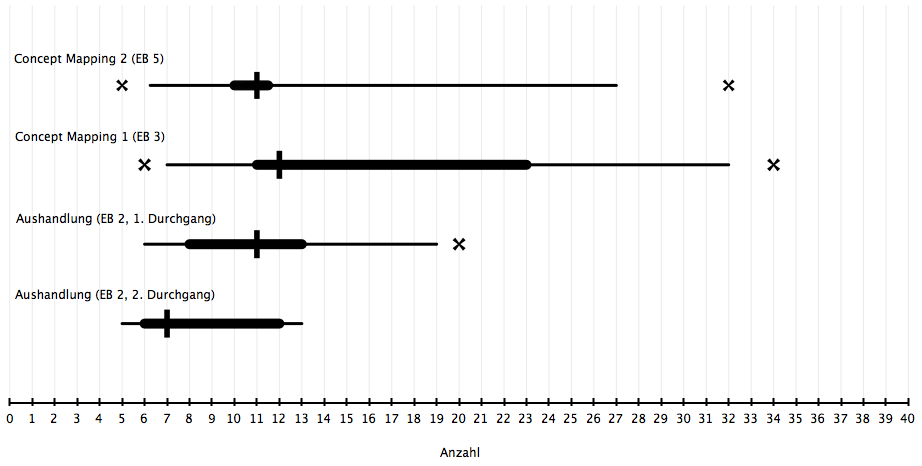
\includegraphics[width=15cm]{img/Evaluierung/elementUsageBlocksOverview.png}
	\caption{Anzahl der verwendeten Elemente -- Übersicht}
	\label{fig:img_Evaluierung_elementUsageBlocksOverview}
\end{figure}

In Abbildung \ref{fig:img_Evaluierung_elementUsageBlocksOverview} ist zu erkennen, dass der Median der Anzahl der verwendeten Elemente zwischen 7 und 12 liegt, wobei die Concept Mapping Aufgabe wegen des nicht explizit vorgegebenen Detaillierungsgrad der Modellierung eine höhere Schwankungsbreite (mit starker Tendenz zu größeren Modellen) aufweist. Zwar war der Detaillierungsgrad der Aushandlungsaufgaben ebenfalls nicht explizit vorgegeben, hier scheint jedoch eine höhere Überstimmung hinsichtlich des angemessenen Detaillierungsgrades gegeben gewesen zu sein. 

Auffällig ist außerdem, dass zwischen den beiden Durchgängen des Aushandlungs-Blocks ein (statistisch allerdings wegen der geringen Stichprobengröße nicht signifikanter ($t=0.16 < t(0.95,8)=2.306$)) Unterschied in der Größe der Modelle (gemessen an der Anzahl der Elemente) gegeben ist. Dies scheint nach Betrachtung der qualitativ erhobenen Daten aus den entsprechenden Videoaufzeichnungen einerseits darauf zurückzuführen zu sein, dass der zweite Durchgang in einer späteren Phase des produktiven Arbeitsprozesses durchgeführt wurde, in dem weniger offene Schritte zu behandeln waren, andererseits scheint durch die bereits etablierte Zusammenarbeitsprozesse generell weniger Abstimmungsbedarf gegeben gewesen zu sein. Dieser Eindruck wird auch durch die generell geringere Modellierungdauer in Durchgang 2 (siehe Abbildung \ref{fig:img_Evaluierung_usageTimeNegotiation}) bestärkt.

\begin{figure}[htbp]
	\centering
		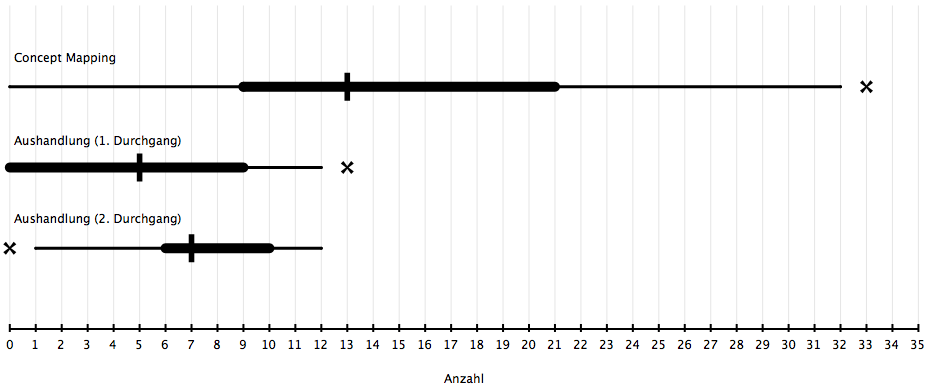
\includegraphics[width=15cm]{img/Evaluierung/elementUsageConnectorsOverview.png}
	\caption{Anzahl der verwendeten Verbindungen -- Übersicht}
	\label{fig:img_Evaluierung_elementUsageConnectorsOverview}
\end{figure}

Eine ähnliche Verteilung wie im Falle der Elemente ergibt sich bei Betrachtung der Anzahl der Verbindungen (siehe Abbildung \ref{fig:img_Evaluierung_elementUsageConnectorsOverview}). Auffällig ist jedoch die gegenüber Durchgang 2 des Aushandlungsblocks geringere Anzahl von Verbindungen in Durchgang 1 während sich die Anzahl der Blöcke zwischen den beiden Modellierungsdurchgängen umgekehrt verhält. Wie in der Überprüfung der Hypothese \ref{hyp:verbinder} in Abschnitt \ref{sub:herstellung_von_verbindern} bestätigt, ist dieses Phänomen auf die Fehlfunktionen und Instabilität der ursprünglichen Funktion zur Herstellung von Verbindungen zurückzuführen, die in Durchgang 1 ausschließlich zur Verfügung stand, während in Durchgang 2 (und auch im Block „Concept Mapping“) bereits die zusätzliche Funktion zur Verbindungsherstellung verfügbar war.

% subsubsection modellgröße (end)

\subsubsection{Vernetzungsgrad} % (fold)
\label{ssub:vernetzungsgrad}

Der Vernetzungsgrad der Modelle („Connectedness“) wurde bereits zur Überprüfung der Hypothese \ref{hyp:verbinder} in Abschnitt \ref{sub:herstellung_von_verbindern} betrachtet, ist jedoch eine Eigenschaft der erstellten Modelle an sich und wird hier deshalb nochmals als deskriptiver Parameter beschrieben.

\begin{figure}[htbp]
	\centering
		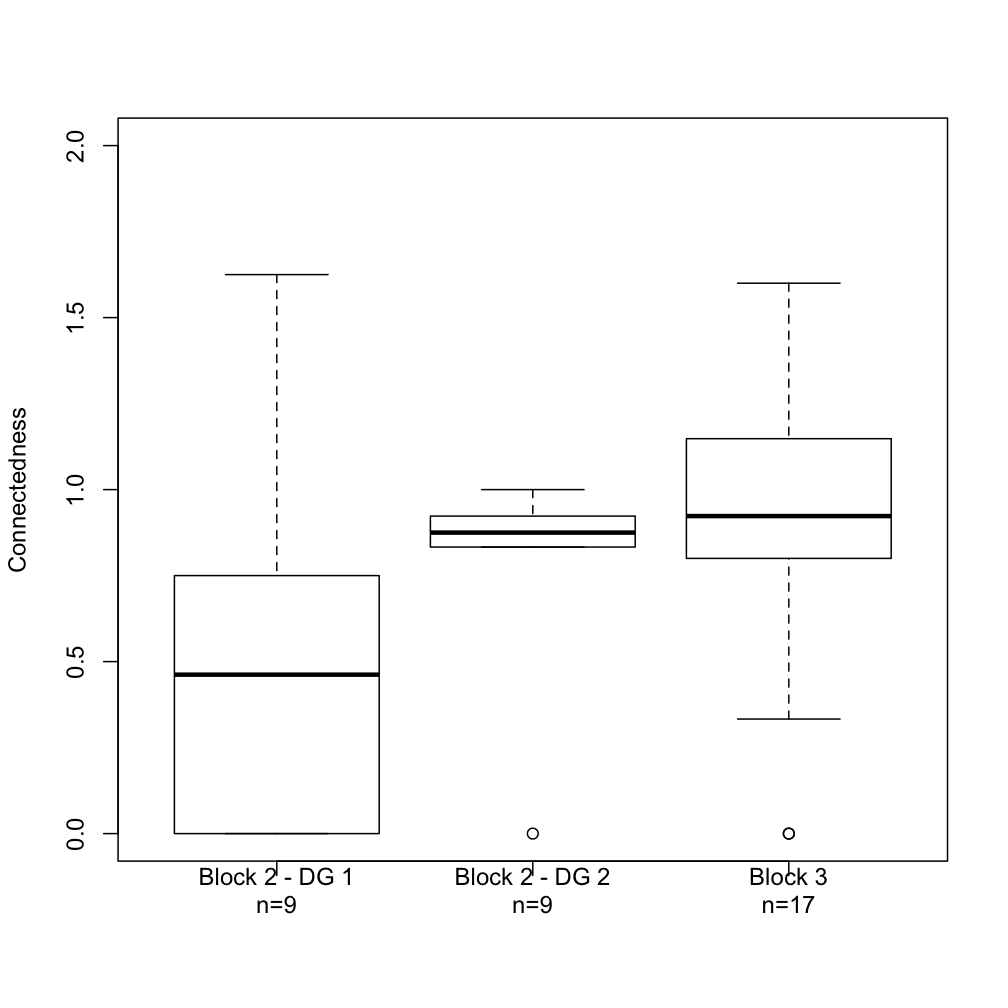
\includegraphics[width=10cm]{img/Evaluierung/connectednessOverview.png}
	\caption{Vernetzungsgrad (Verbindungen / Blöcke) -- Übersicht}
	\label{fig:img_Evaluierung_connectednessOverview}
\end{figure}

Abbildung \ref{fig:img_Evaluierung_connectednessOverview} zeigt die Verteilung des Verhältnisses der Anzahl von Verbindungen und Blöcken in den Evaluierungsblöcken 2 und 3. Zu erkennen ist der oben und in Abschnitt \ref{sub:herstellung_von_verbindern} bereits beschriebene geringere Vernetzungsgrad im ersten Durchgang von Evaluierungsblock 2 der auf die Instabilität und schwierige Verwendbarkeit der ursprünglichen Funktion zur Herstellung von Verbindungen zurückzuführen ist.

Seit der Verfügbarkeit der neuen Funktion zur Herstellung von Verbindungen (also im zweiten Teil von Block 2 sowie in den Blöcken 3, 4 und 5) liegt der Vernetzungsgrad im Mittel immer um 1, wobei in den letzten Blöcken (4 und 5) tendenziell noch höhere Vernetzungsgrade auftreten (Bock 4 im Mittel $1,32$, Block 5 im Mittel XY). Im Falle von Block 4 kann dies teilweise auf die Aufgabenstellungen zurückgeführt werden, die zum Teil starken Fokus auf die Repräsentation von Beziehungen legte (maximaler Vernetzungsgrad in einem Durchgang: $24/8=3$). Bei beiden Blöcken wurden außerdem weitere Stabilisrierungsmaßnahmen in der Interaktions-Erkennungsleistung des Systems vorgenommen, weshalb der gestiegene Vernetzungsgrad zum Teil auch auf die einfachere Herstellbarkeit von Verbindungen zurückgeführt werden kann (siehe wiederum \ref{sub:herstellung_von_verbindern}).

% subsubsection  (end)
% subsection m_durchführung (end)
% section untersuchungsdesign (end)

\section{Ergebnisse} % (fold)
\label{sec:m_ergebnisse}

\subsection{Keine semantische Einschränkung der Externalisierung} % (fold)
\label{sub:keine_semantische_einschränkung_der_externalisierung}

Gegenstand der hier beschriebenen Untersuchung Hypothese \ref{hyp:keine_einschränkung} („Das Werkzeug schränkt Benutzer semantisch nicht bei der Externalisierung ihrer mentalen Modelle ein.“). Als Grundlage dieser Untersuchung dienen die Ergebnisse der Evaluierungsblöcke 2 bis 5, da in diesen die den einzelnen Modellelementen zugewiesene Semantik explizit untersucht wurde. Die Daten hinsichtlich der empfundenen Einschränkung bei der Modellbildung stammen aus der Befragung, die im Rahmen des Evaluierungsblocks 4 durchgeführt wurde. Zusätzlich wurde das Videomaterial aller fünf Evaluierungsblöcke zur Auswertung herangezogen.

\subsubsection{Auswertung} % (fold)

Die „Nicht-Einschränkung“ der Benutzer bei der Externalisierung kann wie in Abschnitt \ref{ssub:keine_semantische_einschränkung_der_externalisierung} beschrieben anhand des Modellierungsverhaltens der Benutzer beurteilt werden. Von Interesse ist hier die Zuweisung von Bedeutung (also semantischer Information) zu den (semantisch nicht vorbelegten) Modellierungselementen. Davon stehen grundsätzlich drei Arten von Blöcken („rot“, „gelb“, „blau“) sowie drei Arten von Verbindern („ungerichtet“, „gerichtet“, „bidirektional“). Erhoben wurde, wie viele Elemente im Verlauf der Modellierung mit Bedeutung belegt wurden, ob die Teilnehmenden mehr als die zur Verfügung stehenden Elemente benötigt hätten und ob ein Element im Modellierungsverlauf mit mehr als einer Bedeutung belegt wurde. 

Zu beachten ist hier, das die Bedeutungsbelegung immer Ergebnis eines Aushandlungsprozesses zwischen mindestens zwei Beteiligten ist. Aus dieser Teiluntersuchung kann also kein Rückschluss auf die individuell empfundene Einschränkung der Externalisierung getroffen werden. Nachdem der Prozess der Bedeutungsfestlegung aber inhärenter Bestandteil der kooperativen Modellbildung ist und die Zielsetzung derselben die Herstellung eines gemeinsamen Verständnisses ist, ist dies im Falle einer tatsächlich kooperativ vorgenommenen Festlegung der Bedeutung nicht als Einschränkung zu sehen. Eine individuell als einschränkend wahrgenommene Situation kann vielmehr dann auftreten, wenn die Bedeutungsfestlegung nicht kooperativ durchgeführt wurde, sondern die Bedeutungen von einem Teilnehmenden vorgegeben wurde. Diese Fälle sind in der folgenden Tabelle separat ausgeführt. Die individuell empfundene Einschränkung wurde außerdem im zweiten Teil der hier beschriebenen Untersuchung mittels einem auf dem \gls{PMS} basierenden Fragebogen sowie einer Auswertung der offenen Fragen zur Eignung des Werkzeugs zur Modellbildung erhoben. 

In der folgenden Tabelle\footnote{EB \ldots Evaluierungsblock, x E.\ldots x Elemente mit Bedeutung belegt, x V. \ldots x Arten von Verbindungen verwendet} ist für jeden Evaluierungsblock ausgeführt, in wie vielen Fällen eine bestimmte Anzahl von Blöcken mit Bedeutung belegt wurde und wie viele Arten von Verbindern benutzt wurden. Unterschiedliche Bedeutungen auf unterschiedlichen Modellebenen (also in eingebetteten Teilmodellen) wurden ohne separaten Unterscheidung mitgezählt.

\todo
\begin{tabular}{| p{1 cm} || p{1cm} | p{1cm} | p{1cm} | p{1.2cm} || p{1cm} | p{1cm} | p{1cm} | p{1.2cm} |}
  \hline
   EB & 1 E. & 2 E. & 3 E. & 4+ E. & 1 V. & 2 V. & 3 V. & 4+ V. \\ \hline
   2 - 1 & 0 & 2 &  9 & 0 & 4 & 1 & 0 & 0 \\ 
   2 - 2 & 1 & 0 &  8 & 0 & 6 & 1 & 0 & 1 \\ 
   3     & 0 & 3 & 14 & 0 & 6 & 4 & 0 & 6 \\ 
   4     & 0 & 2 &  7 & 2 & 3 & 4 & 2 & 1 \\ 
   5     & & & & & & & & \\ \hline
   Ges.  & & & & & & & & \\ \hline
\end{tabular} 
 
In jenen beiden Fällen in Evaluierungsblock 5, in denen 4 oder mehr bedeutungstragende Elemente verwendet wurden, wurden im ersten Fall 6 und im zweiten Fall 7 Elementtypen festgelegt. Beide Modelle enthielten jedoch ineinander verschachtelte Teilmodelle, von denen keines mehr als drei Typen beinhaltete. Jene Fälle, in denen 4 oder mehr verschiedene Arten von Verbindern verwendet wurden, kamen durch den Einsatz benannter Verbinder zustande, mittels derer die Bedeutung der Verbindungen beliebig differenziert werden kann.

Im zweiten Teil der Untersuchung zu dieser Hypothese wurden qualitativ einerseits die expliziten Aussagen der Teilnehmenden ($n_{ges}=147$) hinsichtlich einer eventuellen einschränkenden Wirkung des Werkzeugs gesammelt, andererseits wurden die Videoaufnahmen der Werkzeuganwendungen diesbezüglich ausgewertet. Folgende Punkte mit einschränkender Wirkung konnten hier identifiziert werden (in Klammern jeweils die Quellen sowie die Anzahl des Auftretens der jeweiligen Aussage):
\begin{itemize}
	\item Unterschiedliche Farben von Verbindern wären wünschenswert (Befragung in Block 4, $n=2$)
	\item Drei unterschiedliche Elementtypen sind zu wenig (verbales Feedback von Personen mit praktischen Prozessmodellierungskenntnissen\footnote{Nach diesen Kenntnissen wurde im Rahmen einer Selbsteinschätzung explizit gefragt} in den Blöcken 2 und 4 sowie in nicht formal dokumentieren Modellierungssitzungen mit Prozessmodellierungsexperten\footnote{jeweils nach Eigendeklaration bzw. aus dem professionellen Umfeld der Personen geschlossen} im Rahmen von Demonstrationen auf mehreren Konferenzen, $n=7$)
	\item Dezidierte Elemente zur Modellierung von Verzweigungen und Parallelisierungen im Kontrollfluss wären wünschenswert (verbales Feedback von Personen mit Prozessmodellierungskenntnissen in den Blöcken 2 und 4 sowie in nicht formal dokumentieren Modellierungssitzungen mit Prozessmodellierungsexperten im Rahmen von Demonstrationen auf mehreren Konferenzen, $n=5$)
	\item Selbst festlegbare Formen, Farben und/oder Größen von Modellelementen wären wünschenswert (verbales Feedback von Personen in Block 4 sowie in nicht formal dokumentieren Modellierungssitzungen mit  Strukturaufstellungsexperten\footnote{das Werkzeug scheint sich zur Unterstützung von Strukturaufstellungen \citep{Sparrer02} zu eignen, dies wurde jedoch im Rahmen dieser Arbeit weder als Anwendungsfall vorgesehen, noch formal getestet} im Rahmen von Demonstrationen auf mehreren Konferenzen, $n=3$)
\end{itemize}

Explizite Aussagen zu einer dezidiert „nicht-einschränkenden“ Wirkung bzw. der semantischen Offenheit des Werkzeugs konnten nur in Fällen identifiziert werden, in denen explizit nach diesem Aspekt gefragt wurde. In diesen Fällen wurde der Umfang der Ausdrucksmöglichkeiten durchwegs als ausreichend erachtet. Personen ohne Vorkenntnisse in der Prozessmodellierung empfanden die Anzahl der zur Verfügung stehenden Elemente im Allgemeinen als ausreichend, jene Fälle in denen dies nicht der Fall war, sind oben dokumentiert.

Lediglich in einem\footnote{in Evaluierungsblock 3} der dokumentierten Fälle ($n=65$) waren die Teilnehmenden mit der eigenständigen Wahl der Bedeutung der Elementtypen überfordert und begannen nicht eigenständig zu modellieren. Erst nach einer teilweisen bzw. beispielhaften Vorgabe von 2 Elementtypen durch den Untersuchungsleiter konnten die Teilnehmenden die Modellierung selbständig fortführen. 

Vergleichend ist festzustellen, dass beim Einsatz der Werkzeugs „CMapTools“, das die Anzahl der Elementtypen nicht einschränkt, in Evaluierungsblock 5 ($n=12$) zwischen 1 und 8 Elementtypen verwendet wurden, wobei der Median bei 3 liegt. In je einem Fall wurden 1, 7 und 8 Elementtypen verwendet, in zwei Fällen wurden 3 Elementtypen eingesetzt, in drei Fällen kamen 4 Typen und in vier Fällen 2 Elementtypen zum Einsatz.

\subsubsection{Diskussion} % (fold)

Betrachtet man die Ergebnisse der quantitativen Auswertung der Einsätze des Werkzeugs in den Evaluierungsblöcken 2 bis 5, so scheint die gegebene Ausdrucksstärke für die Modellierung weitgehend ausreichend zu sein. Dieser Eindruck relativiert sich bei einer vergleichenden Betrachtung mit einem computerbasierten, semantisch vollständig offenen Werkzeug sowie bei Betrachtung der qualitativen Auswertung der Benutzeraussagen sowie der Videoaufnahmen. 

In der vergleichend durchgeführten Studie in Evaluierungsblock 5 zeigt sich, dass bei keiner Einschränkung der Anzahl der Modellelementtypen in mehr als der Hälfte der Fälle mehr als die im hier betrachteten Werkzeug zur Verfügung stehenden drei Elementtypen verwendet werden. Dies scheint darauf hinzudeuten, dass sich die Teilnehmenden an der beschränkten Anzahl der zur Verfügung stehenden Elemente orientieren, auch wenn dies -- wie aus den Aussagen der Teilnehmenden bei der ex-post-Befragung ersichtlich -- bis auf einige Ausnahmen nicht als Einschränkung wahrgenommen wird.

Aus den qualitativen Rückmeldungen zur Modellierung zeigt sich außerdem, dass Personen, die in ihrer täglichen Arbeit aktiv mit Prozessmodellierung beschäftigt sind, bei Aufgabenstellungen, die aufgrund ihrer Fragestellung zu Ablaufbeschreibungen führen, eher die Verwendung von mehr als drei Elementtypen bevorzugen würden. Personen, denen Prozessmodellierung fremd ist oder deren Erfahrung damit sich auf eine einmalige, länger zurückliegende Ausbildung beschränkt, konnten ihre Modelle zu ablauforientierten Fragestellungen ohne Ausnahme mit maximal drei Elementtypen abbilden. Bei nicht ablauforientierten Fragestellungen ist diese Unterscheidung nicht zu beobachten.

In Einzelfällen wurden außerdem weitere Wünsche zur Steigerung der Ausdrucksmöglichkeiten im Modell geäußert. Neben dem Wunsch nach unterschiedlich einfärbbaren Verbindungen zwischen Elementen wurde vor allem der Wunsch nach der Verwendung beliebiger Gegenstände als Modellelemente mehrfach geäußert, was das Einbringen von Repräsentation aus der alltäglichen Arbeitspraxis anstelle der abstrakten Modellelemente erlauben würde.

Unter Berücksichtigung dieser Einschränkungen kann die hier betrachtete Hypothese mit Vorbehalten bestätigt werden. Tatsächlich scheint das Werkzeug bis auf wenige Ausnahmen nicht als semantisch einschränkend wahrgenommen zu werden, die Ergebnisse der vergleichenden Studie weisen aber auf eine einschränkende Wirkung durch die auf drei beschränkte Anzahl von Elementtypen hin.

\subsubsection{Ergebnis} % (fold)

\textbf{Die Hypothese \ref{hyp:keine_einschränkung} kann in der Untersuchung mit Vorbehalten angenommen werden.} Die Verwendung des Werkzeugs zur Modellierung scheint (bis auf wenige Ausnahmen) nicht als semantisch einschränkend wahrgenommen zu werden. Die vergleichende Studie aus Evaluierungsblock 5 deutet allerdings auf eine einschränkende Wirkung durch die auf drei beschränkte Anzahl von Elementtypen hin.

% subsection keine_semantische_einschränkung_der_externalisierung (end)

\subsection{Repräsentation beliebig umfangreicher Modelle} % (fold)
\label{sub:repräsentation_beliebig_komplexer_modelle}

Gegenstand der hier beschriebenen Untersuchung Hypothese \ref{hyp:beliebige_komplexität} („Das Werkzeug ermöglicht die Repräsentation beliebig umfangreicher Modelle.“). Als Grundlage dieser Untersuchung dienen die Ergebnisse der Modellbildung in Evaluierungsblock 3 und 5 sowie die Befragungen in den Evaluierungsblöcken 1 bis 5.

\subsubsection{Auswertung} % (fold)

Von Interesse ist bei der Prüfung dieser Hypothese der Vergleich des Umfangs von Modellen, die mit dem hier vorgestellten Werkzeug erstellt wurden, mit Modellen, die mit einem bezogen auf die Größe der Arbeitsfläche unbeschränkten Werkzeug erstellt wurden. Diese vergleichende Studie wurde im Rahmen der Untersuchungen in Block 5 durchgeführt. Als Metrik zum Vergleich der Modellgrößen wurde die Anzahl der Modellelemente verwendet. Abbildung \ref{fig:img_Evaluierung_ElementeConceptMapping2} zeigt eine Gegenüberstellung der Modellgrößen bei Verwendung der „CMapTools“ als die Größe nicht beschränkendes Werkzeug und dem hier vorgestellten System\footnote{In allen Boxplots gilt folgende Notation: 
\begin{itemize}
	\item breite horizontale Linie: Bereich zwischen 25\%- und 75\%-Quantil
	\item breite vertikale Linie: Median
	\item linke schmale Linie: Bereich zwischen 2,5\%- und 25\%-Quantil
	\item rechte schmale Linie: Bereich zwischen 75\%- und 97,5\%-Quantil
	\item Kreuze: Ausreißer (außerhalb 2,5\%- und 97,5\%-Quantil)
\end{itemize}
}.

\begin{figure}[htbp]
	\centering
		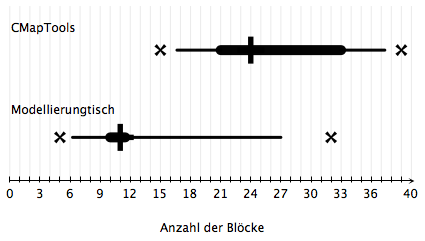
\includegraphics[width=10cm]{img/Evaluierung/ElementeConceptMapping2.png}
	\caption{Gegenüberstellung der Modellgrößen in Evaluierungsblock 5}
	\label{fig:img_Evaluierung_ElementeConceptMapping2}
\end{figure}

Die Betrachtung der Ergebnisse zeigt, dass die Modelle, die mittels der „CMapTools“ erstellt wurden ($M=25.92, SD=7.04, N=12$), signifikant umfangreicher waren (einseitiger t-Test für zwei ungepaarte Stichproben ungleicher Varianz $t(21)=4.74, p<=0.001$), als jene Modelle, die mittels dem hier vorgestellten System erstellt wurden ($M=12.18, SD=6.84, N=11$).

In den Evaluierungsblöcken 3 und 5 wurden insgesamt 30 Modellierungsdurchgänge durchgeführt, deren Ergebnis aufgrund der Aufgabenstellung bei detaillierte Modellierung mehr als 15 Modellierungselement enthalten müsste (siehe vergleichende Ergebnisse aus Block 5). In insgesamt 7 Fällen wurden mehr als 15 Elemente verwendet ($15<x<=20: 1, 20<x<=25: 2, 25<x<=30: 2, x>30: 2$), der Median der Anzahl der Elemente liegt bei 11 ($M=14.68, SD=7.90, N=30$). Die Möglichkeit der Einbettung von Teilmodellen wurde insgesamt in 8 Modellierungsdurchgängen genutzt, davon war in drei Fällen die Gesamtanzahl der Elemente geringer als 15 (womit eine rein semantische Strukturierung vorliegt und keine Steigerung der Modellumfangs vorgenommen wurde).

Neben der vergleichenden Studie wurde in allen Evaluierungsblöcken der subjektive Eindruck der Teilnehmenden nach einer etwaig einschränkenden Wirkung hinsichtlich des Umfangs der Modelle gefragt ($n_{ges}=147$). Insgesamt 43 Teilnehmende empfanden die Modellierungsoberfläche als zu klein um die gewünschten Sachverhalte abzubilden. Von insgesamt 9 Teilnehmenden wurde explizit der Wunsch nach kleineren Elementen geäußert, um umfangreichere Modelle abbilden zu können. Von 23 Teilnehmenden wurde die Visualisierung der Verbindungen kritisiert („unübersichtlich“, „nur eine Verbindung zwischen zwei Blöcken möglich“), was dazu geführt hätte, dass die Modelle nicht wie ursprünglich intendiert aussähen.

\subsubsection{Diskussion} % (fold)

Sowohl die quantitativen Ergebnisse auf Evaluierungsblock 5 als auch die qualitativen Ergebnisse weisen darauf hin, dass die physische Realisierung der Modells, die mit eine Beschränkung der Modellierungsoberfläche einher geht, die Abbildung beliebig umfangreicher Modelle nicht erlaubt.

Bei der Gegenüberstellung des quantitativen Teils der Studie mit den qualitativen Aussagen der Teilnehmenden fällt auf, dass -- wie bereits bei der Diskussion der Hypothese \ref{hyp:keine_einschränkung} in Abschnitt \ref{sub:keine_semantische_einschränkung_der_externalisierung} -- die subjektive Wahrnehmung der Einschränkung weniger stark ausgeprägt ist als die vermutete tatsächliche Einschränkung, auf die aufgrund der quantitativen Daten geschlossen werden kann. Tatsächlich ist jedoch der Anteil der Teilnehmer, die das Modell nicht so umfangreich wie intendiert abbilden konnten, höher als jener die sich in der semantischen Ausdrucksstärke eingeschränkt fühlten.

Aus den qualitativen Aussagen ist zu erkennen, das der vorrangige Grund der Beschränkung des Modellumfangs die eingeschränkte Größe der Modellierungsoberfläche ist. Die Möglichkeit zur Einbettung von Teilmodellen zur Steigerung des Umfangs wurde nur in einem Sechstel der Fälle verwendet, was darauf hindeutet, dass diese Funktion keinen Ersatz für eine unbeschränkt große Modellierungsoberfläche (auf einer Abstraktionsebene) darstellt.

Insgesamt kann aufgrund der Ergebnisse der Untersuchung die Hypothese \ref{hyp:beliebige_komplexität} nicht bestätigt werden.

\subsubsection{Ergebnis} % (fold)

\textbf{Die Hypothese \ref{hyp:beliebige_komplexität} kann in der Untersuchung nicht bestätigt werden.} Modelle, die mit dem hier vorgestellten Werkzeug erstellt wurden, weisen bei identischer Aufgabenstellung einen signifikant geringeren Umfang auf als Modelle, die mit einem Werkzeug mit nicht beschränkter Arbeitsfläche erstellt wurden. Auch das qualitative Feedback der Benutzer deutet darauf hin, dass eine vollständige Abbildung eines Modells (und damit die Erstellung eines Modells mit größerem Umfang) nicht bzw. nur umständlich möglich ist.

% subsection repräsentation_beliebig_komplexer_modelle (end)

% subsection abstimmung_individueller_modelle (end)

\subsection{Reflexion des Modellierungsverlaufs} % (fold)
\label{sub:reflexion_des_modellierungsverlaufs}

Gegenstand der hier beschriebenen Untersuchung ist Hypothese \ref{hyp:historie} („Die Reflexion des Modellierungsverlaufs ermöglicht das Verständnis der dem Modell zugrundeliegenden mentalen Modelle.“). Als Grundlage dieser Untersuchung dienen die Ergebnisse der Evaluierungsblöcke 2 und 4.

\subsubsection{Auswertung} 

\subsubsection{Diskussion} 

\subsubsection{Ergebnis} 


\subsection{Wirkung auf die Kooperation bei der Modellerstellung} % (fold)
\label{sub:wirkung_auf_die_kooperation_bei_der_modellerstellung}

Gegenstand der hier beschriebenen Untersuchung Hypothese \ref{hyp:stärkere_kooperation} („Die Verwendung des Werkzeugs führt zu stärkerer Kooperation bei der Modellerstellung als die Verwendung von bildschirm-basierten Werkzeugen.“). Als Grundlage dieser Untersuchung dienen die Videoaufnahmen sowie die Ergebnisse der Teilnehmerbefragung des Evaluierungsblocks 5.

\subsubsection{Auswertung} % (fold)

Zur Beurteilung des Ausmaßes der Kooperation lässt sich aus dem Prozess der Modellbildung heraus an der Verteilung der Modellierungszeit zwischen den Teilnehmern, den Anzahl der Initiativwechsel sowie dem Anteil von Diskussionszeit an der Gesamtmodellierungsdauer messen.

Die Zeitverteilung zwischen den Teilnehmern betrug bei der Durchführung mittels CMapTools bei einer Gruppengröße von 2 Personen für Teilnehmer A im Schnitt 19 Minuten 21 Sekunden ($SD=8:11, N=11$) und für Teilnehmer B im Schnitt 14 Minuten 44 Sekunden ($SD=5:54, N=11$). Setzt man diese Werte zueinander ins Verhältnis ergibt sich ein Anteil von $56.88\%$ für Teilnehmer A und $43.12\%$ für Teilnehmer B. Bei jener Anwendung, die von drei Personen durchgeführt wurde ergab sich die Verteilung 20 min - 12 min - 8 min. 

Bei der Durchführung am Modellierungstisch ergab sich bei einer Gruppengröße von 2 Personen für Teilnehmer A im Schnitt 17 Minuten und 18 Sekunden ($SD=6:59, N=9$) und für Teilnehmer B im Schnitt 13 Minuten 12 Sekunden ($SD=6:01, N=9$). Setzt man diese Werte zueinander ins Verhältnis ergibt sich ein Anteil von $57.52\%$ für Teilnehmer A und $42.48\%$ für Teilnehmer B. Bei den beiden Anwendungen, an denen drei Personen beteiligt waren, ergab sich eine Verteilung von 5 min - $2.5$ min - $2.5$ min bzw. 20 min - 10 min - 3 min. 

Der Unterschied zwischen den Anteilen im Verhältnis zur gesamten Modellierungsdauer (${t_{TN A} - t_{TN B}}/t_{ges}$\footnote{Als Teilnehmer A wird immer jener Teilnehmer bezeichnet, der den höheren Zeitanteil in der Modellierung in Anspruch nahm.}, lediglich Anwendungen mit 2 Beteiligten wurden berücksichtigt) beträgt bei der Anwendung der CMapTools im Schnitt $0.138$ ($SD=0.086, N=11$) und am Modellierungstisch im Schnitt $0.151$ ($SD=0.087, N=9$). Zwischen diesen beiden Werten kann kein signifikanter Unterschied festgestellt werden (zweiseitiger Wilcoxon-Test: $W=51, p=0.8588, N=20$).

Hinsichtlich der Wechsel der Initiative waren bei der Durchführung der Modellierung mittels CMapTools ($N=12$) 8 Fälle zu beobachten, in denen ein Teilnehmer exklusiven Zugriff auf die Eingabemedien über den gesamten Verlauf der Modellierung hatte. In 2 Fällen fanden zwei Initiativ-Wechsel statt, in jeweils 1 einem Fall fanden 4 bzw. 8 Initiativ-Wechsel statt. Bei der Durchführung der Modellierung it dem hier vorgestellten System ($N=11$) wurde in 7 Fällen simultan an der Benutzungsschnittstelle gearbeitet, es konnten keine Initiativ-Wechsel im Sinne obiger Definition festgestellt werden. In 2 Fällen wurden je 2 Wechsel der Initiative festgestellt, in zwei Fällen kam es zu keinem Initiativ-Wechsel.

Der Anteil von Diskussionszeit an der Gesamtmodellierungsdauer betrug bei der Durchführung mittels CMapTools im Schnitt $57.15\%$ ($SD=7.49\%, N=12$) und war damit signifikant niedriger (einseitiger Wilcoxon-Test: $W=120, p<0.001, N=23$) als der Diskussionsanteil bei der Arbeit am Modellierungstisch mit im Schnitt $76.08\%$ ($SD=8.84\%, N=11$).

\todo qualitative Daten aus den Fragebögen!

\subsubsection{Diskussion} % (fold)

Die Verteilung der Modellierungsdauer zwischen den Teilnehmern als erstgenannter Indikator für funktionierende Kooperation zwischen den Teilnehmern zeigt keine signifikanten Unterschiede zwischen den beiden eingesetzten Werkzeugen. In beiden Fällen zeigt sich eine im Schnitt annähernde Gleichverteilung der Modellierungsdauer zwischen den Teilnehmern, was darauf hinweist, dass eine kooperative Modellierung sowohl mit dem Werkzeug CMapTools als auch mit dem hier vorgestellten Modellierungstisch möglich ist.

Betrachtet man jedoch die Anzahl der physischen Initiativwechsel, zeigt sich, dass die Möglichkeit des nicht-exklusiven Zugriffs auf die Benutzungsoberfläche des Modellierungtisches von den Teilnehmern genutzt wird und dazu führt, dass das die Manipulation des externalisierten Modells unmittelbar von mehr als einem Teilnehmer durchgeführt wird. Im Falle der mit der Maus und Tastatur bedienten CMapTools führt in den meisten Anwendungen ein Teilnehmer exklusiv die Manipulation des Modells durch. Durch den Wegfall des inhaltlichen „Filters“, den der manipulierende Teilnehmer potentiell bewusst oder unbewusst einführen kann, ist am Modellierungstisch eine unmittelbarere Kooperation bei der Modellerstellung möglich.

Auch die Verteilung zwischen der zur eigentlichen Modellerstellung benötigten Zeit und jener Zeit, die zum inhaltlichen Austausch über den Modellierungsgegenstand aufgewendet wird, weißt darauf hin, dass die Kooperation durch den Einsatz des Modellierungstisches im Vergleich zu den bildschirmbasierten CMapTools gestärkt wird.

\todo Fragebögendaten!

\subsubsection{Ergebnis} % (fold)

\textbf{Die Hypothese \ref{hyp:stärkere_kooperation} kann auf Basis der Untersuchung bestätigt werden.} Während die Verteilung des Zeitanteils zwischen den Modellierungsteilnehmern keinen signifikanten Unterschied zwischen den beiden verglichenen Systemen aufweist, zeigt sowohl der Vergleich der Initiativ-Wechsel als auch der Anteil an zum inhaltlichen Austausch aufgewandter Zeit einen signifikanten Vorteil hinsichtlich der Kooperationsförderung für den Modellierungstisch. Auch die qualitativen Daten aus der Befragung der Teilnehmer weisen darauf hin, dass der Einsatz des hier vorgestellten Systems als eher kooperationsfördernd wahrgenommen wurde als die Verwendung der CMapTools.

% subsection wirkung_auf_die_kooperation_bei_der_modellerstellung (end)

\subsection{Abbildung von Zusammenhängen ohne Verbinder} % (fold)
\label{sub:abbildung_von_zusammenhängen_ohne_verbinder}

Gegenstand der hier beschriebenen Untersuchung Hypothese \ref{hyp:keine_verbinder} („Zur Abbildung von Zusammenhängen ist die Verwendung von Verbindern nicht notwendig.“). Als Grundlage dieser Untersuchung dienen die Befragungen sowie die Videoaufnahmen der Evaluierungsblöcke 1 bis 5.

\subsubsection{Auswertung} % (fold)

In insgesamt 18 von den in allen 5 Evaluierungsblöcken 64 erstellten Modellen (für eine detaillierte Aufstellung siehe Abschnitt \ref{sub:repräsentation_diagrammatischer_modelle}) wurden keine Verbinder zur Darstellung von Zusammenhängen zwischen Elementen verwendet. Von diesen 18 Modellen wurden 9 Modelle (in den Evaluierungsblöcken 2 und 3) während der Modellierung von allen Beteiligten kommunikativ interpretiert. Die Teilnehmenden wurden unmittelbar nach Abschluss der Modellbildung über ihre subjektive Wahrnehmung der Übereinstimmung des Verständnisses über den abgebildeten Sachverhalt befragt. Alle Teilnehmer ($n_{ges}=21$) gaben an, subjektiv ein gemeinsames Verständnis erreicht zu haben. Diese Angaben decken sich mit den Auswertungen der Modellierungsverläufe in diesen Durchgängen, in denen in 3 von 9 Fällen während der Modellierung der Eindruck entstand, dass Teile der Modelle unterschiedlich interpretiert wurden. Diese unterschiedlichen Interpretationen wurden jedoch in allen Fällen im weiteren Verlauf der Modellierung erkannt und so abgestimmt, das ein übereinstimmendes Verständnis hergestellt werden konnte.

Jene 9 Modelle, die in Evaluierungsblock 1 erstellt wurden, wurden von Dritten interpretiert. Die Interpretation wurde dabei den ursprünglichen Modellerstellern rückgespiegelt, die wiederum zu beurteilen hatten, ob die Interpretation den ursprünglich repräsentierten Sachverhalt korrekt wiedergibt. Dies war in allen 9 Modellierungsdurchgängen der Fall. Die Abbildungen  \ref{fig:img_Evaluierung_modell_verbinder_unwichtig1} und \ref{fig:img_Evaluierung_modell_verbinder_unwichtig2} zeigen Beispiele für Modelle, in denen die korrekte Intepretation auch ohne die Darstellung von Verbindern möglich war.

\begin{figure}[htbp]
	\centering
		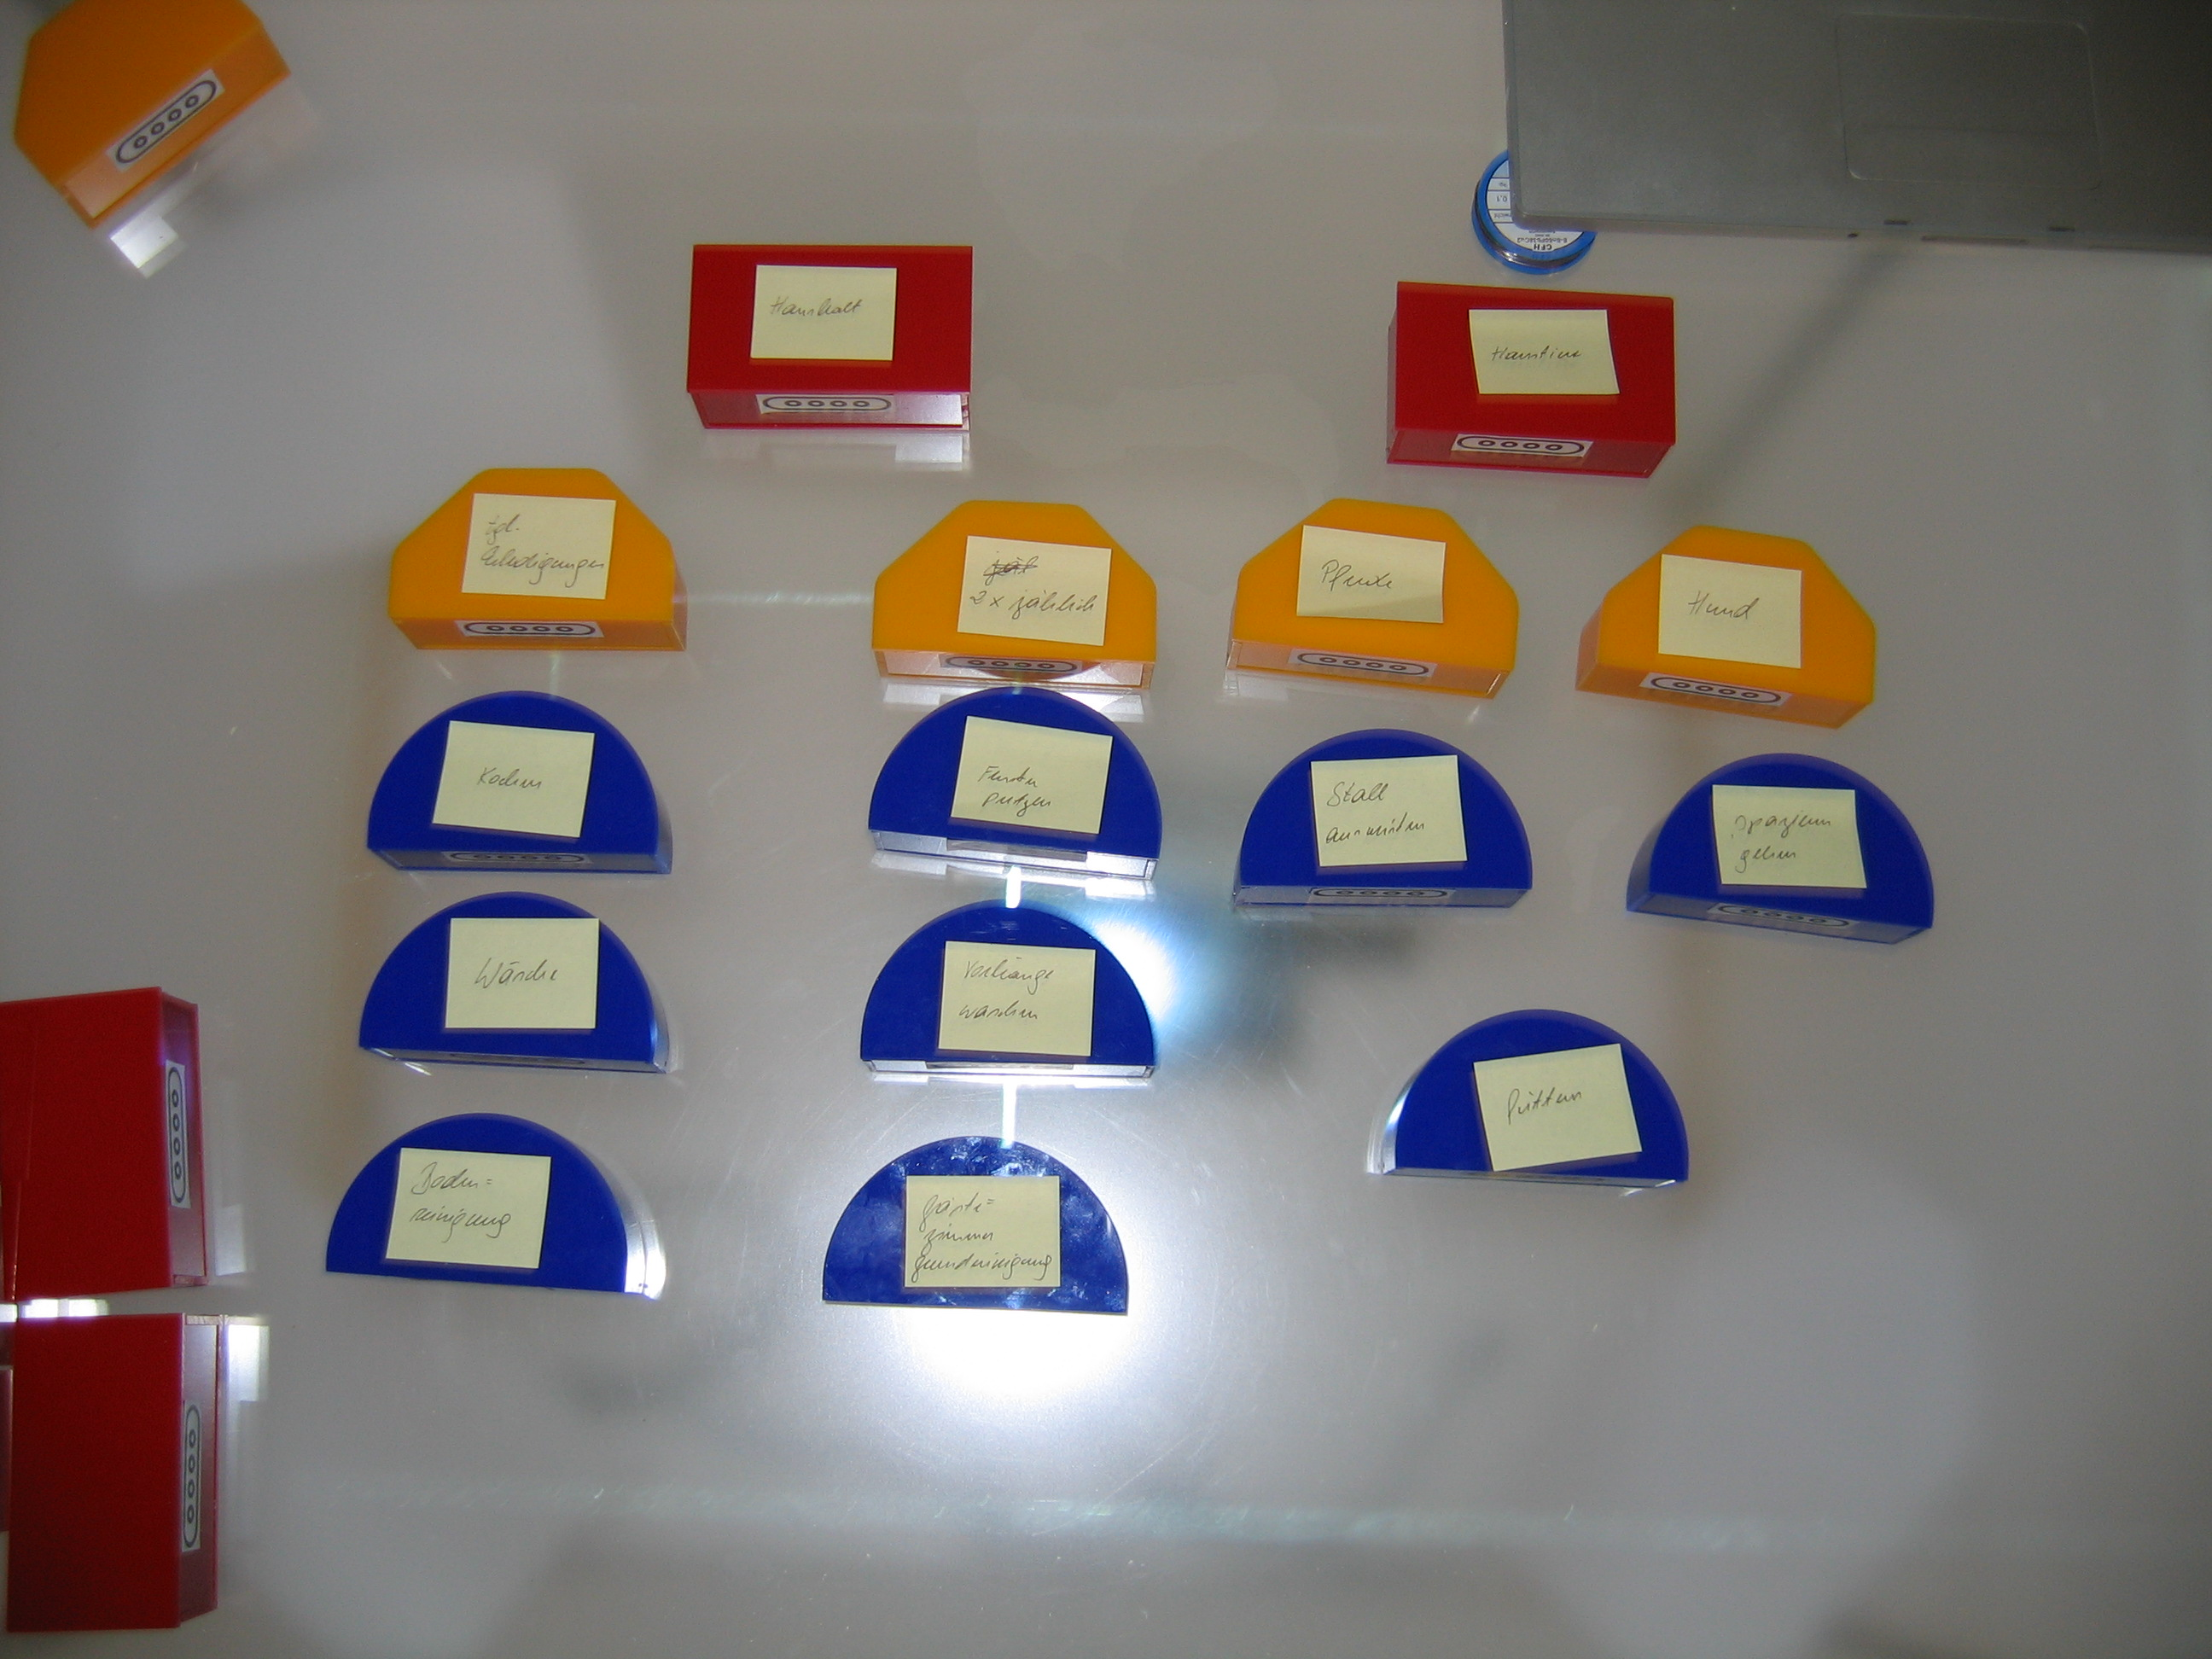
\includegraphics[width=10cm]{img/Evaluierung/modell_verbinder_unwichtig1.JPG}
	\caption{Korrekt intepretierbares Modell ohne Verbinder (hierarchisch)}
	\label{fig:img_Evaluierung_modell_verbinder_unwichtig1}
\end{figure}

\begin{figure}[htbp]
	\centering
		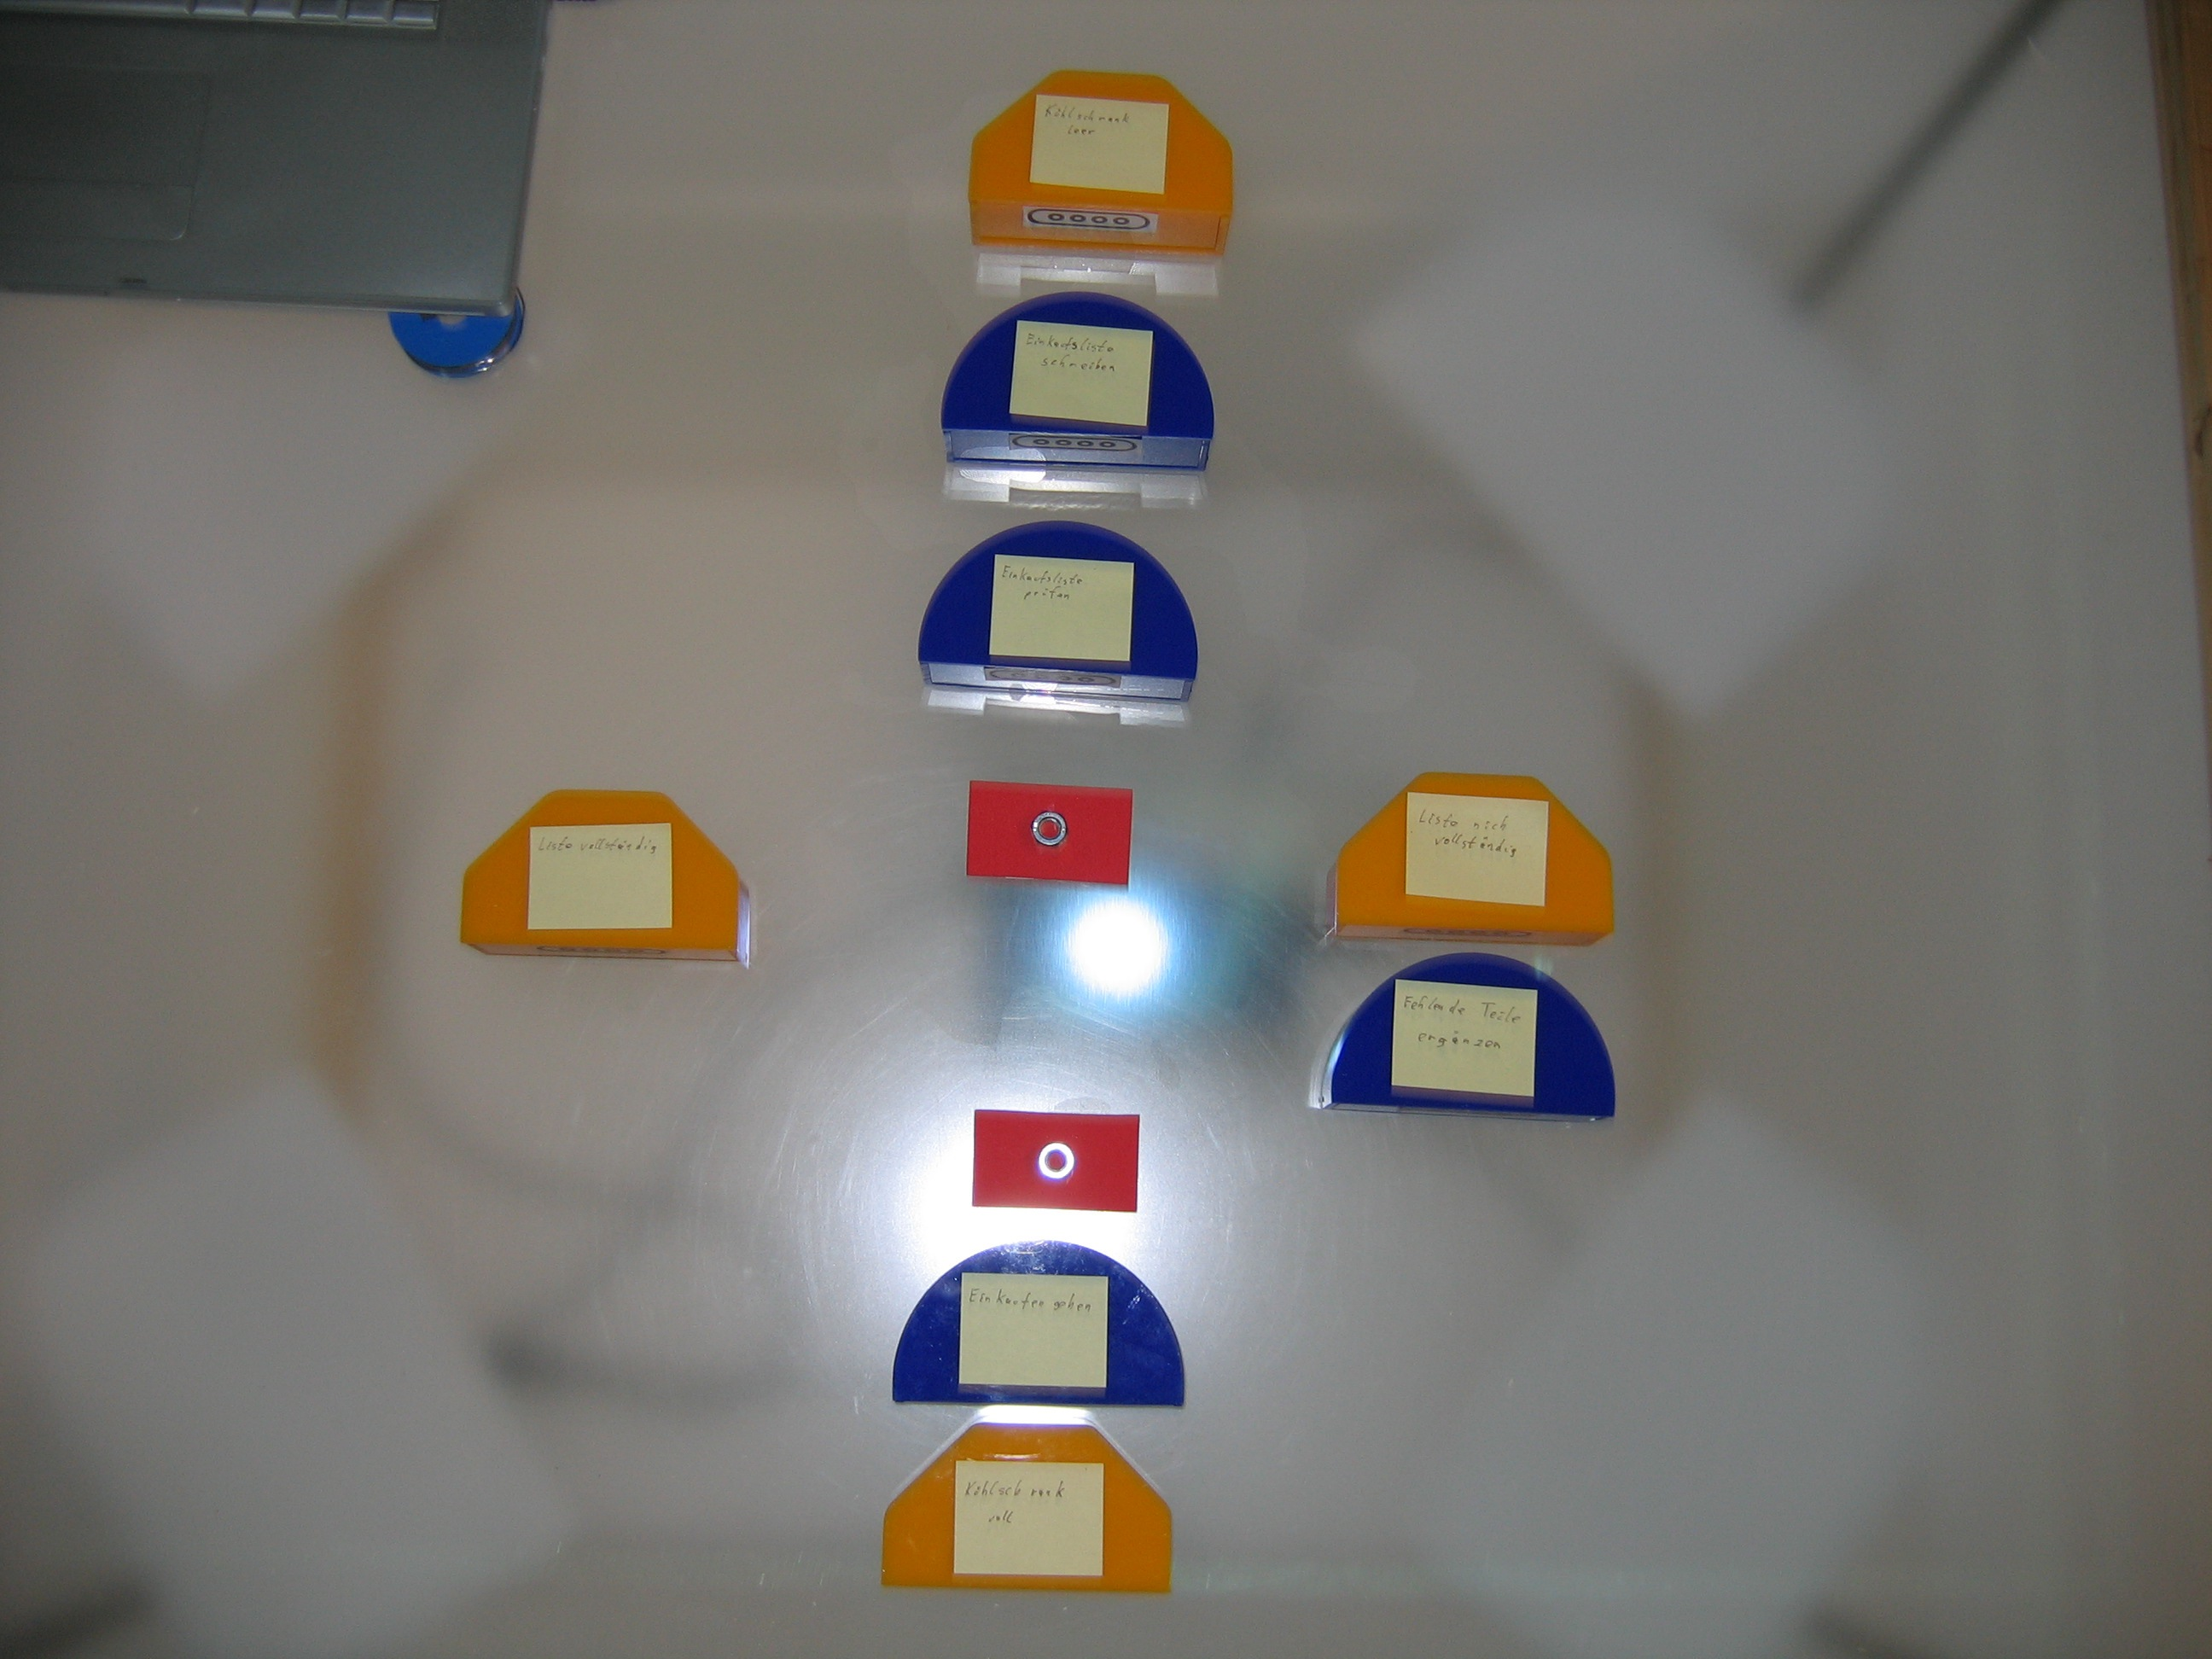
\includegraphics[width=10cm]{img/Evaluierung/modell_verbinder_unwichtig2.JPG}
	\caption{Korrekt intepretierbares Modell ohne Verbinder (ablauforientiert)}
	\label{fig:img_Evaluierung_modell_verbinder_unwichtig2}
\end{figure}

Die übrigen 46 Modelle, in denen Verbinder verwendet wurden, wurden einer nachgelagerten Interpretation durch den Leiter der Studiendurchführung\footnote{dem Verfasser dieser Arbeit} unterzogen, der an der Durchführung von 17 Modellierungsdurchgängen als Untersuchungsleiter beteiligt war (die übrigen 29 Modellierungsdurchgänge wurden im Rahmen von Diplomarbeiten erfasst, wobei die jeweiligen Diplomanden als Untersuchungsleiter auftraten). Bei dieser Interpretation wurden im ersten Schritt für jedes Modell die verwendeten Verbinder entfernt und versucht, den Modellinhalt zu interpretieren. In einem zweiten Schritt wurden die Verbinder wieder eingeblendet und die Interpretation mit dem nun vollständigen Modell verglichen. Dabei ergaben sich in 15 Fällen Unterschiede in der Interpretation, die ausschließlich auf die Verwendung von Verbindern zurückzuführen war. In den übrigen 36 Fällen explizierten bzw. bestätigten die erstellten Verbindungen die durch die räumliche Anordnung der Modellierungselemente implizit ausgedrückten Zusammenhänge. Dabei ist zu anzuführen, dass in 13 der insgesamt 46 Modelle benannte Verbinder verwendet wurden (die übrigen 33 Modelle enthielten lediglich unbenannte Verbinder). Von diesen 13 Modellen konnten 4 auch ohne die Darstellung der Verbinder korrekt (im Sinne der obigen Ausführungen) interpretiert werden. Demnach führte die Entfernung der Verbinder in 6 der 33 Modelle mit unbenannten Verbindern zu unvollständigen bzw. fehlerhaften Interpretationen. Abbildung \ref{fig:img_Evaluierung_modell_verbinder_wichtig} zeigt ein Beispiel für ein Modell, in dem die Entfernung der Verbinder zu einer unvollständigen Interpretation des abgebildeten Inhalts führte.

\begin{figure}[htbp]
	\centering
		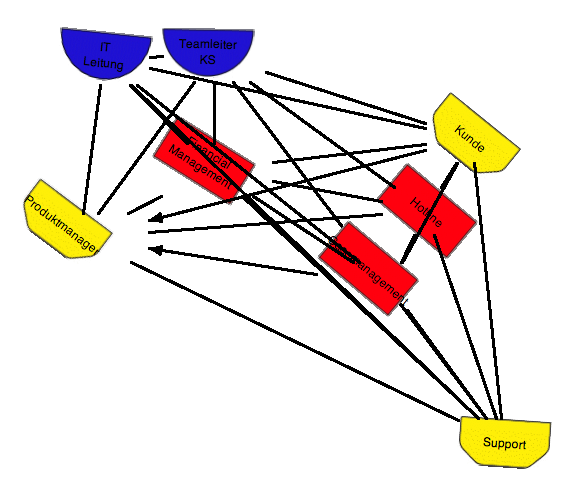
\includegraphics[width=10cm]{img/Evaluierung/modell_verbinder_wichtig.png}
	\caption{Bei Vernachlässigung der Verbinder nur unvollständig interpretierbares Modell}
	\label{fig:img_Evaluierung_modell_verbinder_wichtig}
\end{figure}

\subsubsection{Diskussion} % (fold)

Das weitgehende Fehlen von Verbindern ist in den ersten beiden Evaluierungsblöcken sowie Teilen des Evaluierungsblocks 3 auf die mangelhafte Funktion der Verbindungsherstellung durch Benutzer zurückzuführen (siehe Prüfung der Hypothese \ref{hyp:diagmodelle} in Abschnitt \ref{sub:repräsentation_diagrammatischer_modelle}). Trotzdem war es den Teilnehmenden möglich, ein gemeinsames Verständnis über die abgebildeten Zusammenhänge zu entwickeln. Auch bei der Interpretation durch Dritte, die am Entstehungsprozess des Modells nicht beteiligt waren, traten keine Missverständnisse auf. Dies gilt sowohl für ablauf-orientierte Modelle (in Evaluierungsblock 1 und 2) als auch für Concept-Map-artige Modelle (in Evaluierungsblock 3).

Insofern scheint die Hypothese bestätigt werden zu können. Diese Annahme ist insofern zu relativieren, als dass den Evaluierungsblöcken 3, 4 und 5 insgesamt 15 Modellierungsdurchgänge identifiziert werden konnten, in denen die Verwendung von Verbindungen den Modellen Bedeutung hinzufügt, die ohne diese auch implizit nicht vorhanden gewesen wäre. Eine vorbehaltslose Annahme der Hypothese erschient deshalb nicht gerechtfertigt.

Hypothese \ref{hyp:keine_verbinder} kann unter Berücksichtigung der obigen Ausführungen damit nicht bestätigt werden. Während in vielen Fällen die ausschließliche räumliche Anordnung von Modellierungselementen ausreichend zu sein scheint, um die beabsichtigte Bedeutung zu kommunizieren, konnten Fälle identifiziert werden, in denen dies nicht möglich war.

\subsubsection{Ergebnis} % (fold)

\textbf{Die Hypothese \ref{hyp:keine_verbinder} kann auf Basis der Untersuchung nicht bestätigt werden.} Während zu Bildung eines einheitlichen Verständnisses in vielen Fällen die implizite Abbildung von Zusammenhängen durch räumliche Konfiguration der Modellierungselemente ausreichend erscheint, konnten Fälle identifiziert werden, in denen die explizite Repräsentation von Verbindern dem Modell Bedeutung hinzufügte, die ohne Darstellung derselben nicht kommunizierbar gewesen wäre.

% subsection abbildung_von_zusammenhängen_ohne_verbinder (end)
% section m_ergebnisse (end)

\section{Zusammenfassung} % (fold)
\label{sec:m_zusammenfassung}

In diesem Kapitel wurde die Evaluierung des Aspektes der Modellierung mit dem hier vorgestellten Werkzeug beschrieben. Die hier betrachteten Hypothesen beschäftigen sich mit dem Modellierungsergebnis ansich sowie dem Prozess der Modellerstellung. In Abgrenzung dazu wurde in Kapitel \ref{cha:eval_werkzeug} die Verwendung des Werkzeugs im Allgemeinen sowie dessen Verständlichkeit geprüft. Kapitel \ref{cha:eval_aw} beschäftigt sich hingegen mit der Rückwirkung der Modellierung bzw. der Modelle auf die eigentlichen Betrachtungsgegenstände (also etwa operative Arbeitsabläufe).

Im Rahmen dieses Kapitels wurden drei aus der Aufgabenstellung begründbare Hypothesen und eine explorativ während der Evaluierung gebildete Hypothese getestet. Die ersten beiden Hypothesen beschäftigen sich mit einer eventuell einschränkenden Wirkung des Werkzeugs auf die Modellbildung. Wie in den Anforderungen \ref{anf:nicht_vorgegebene_semantik_der_modellierungselemente} und \ref{anf:bearbeitung_von_beliebig_komplexen_modellen} formuliert, muss das Werkzeug zur Unterstützung von „Articulation Work“ einerseits semantische Offenheit bei der Modellierung bieten (d.h. die Modellierenden nicht bei der Abbildung der eigenen Konzeptualisierung des abzubildenden Sachverhaltes einschränken) und andererseits die Abbildung beliebig umfangreicher Modelle erlauben. 

Hypothese \ref{hyp:keine_einschränkung} („Semantische Offenheit“) konnte dabei insofern bestätigt werden, als dass die Teilnehmenden das Werkzeug nur in Einzelfällen als semantisch einschränkend empfanden. Der Vergleich mit einem semantisch vollständig offenen Werkzeug, dass die Anzahl der Elementtypen im Gegensatz zum vorliegenden Werkzeug nicht beschränkt, deutet jedoch darauf hin, dass in manchen Anwendungsfällen tatsächlich mehr als die drei im Werkzeug semantisch belegbaren Elementtypen zum Einsatz kommen sollten.  

Hypothese \ref{hyp:beliebige_komplexität} („Beliebiger Modellumfang“) konnte im Rahmen der Untersuchung nicht bestätigt werden. Die beschränkte Größe der Modellierungsoberfläche scheint einschränkend auf den Modellumfang zu wirken, die Möglichkeit der Einbettung von Teilmodellen ist dabei kein adäquater Ersatz. In einer vergleichenden Studie mit einem die Arbeitsfläche nicht beschränkenden Werkzeug wurden bei identischer Aufgabenstellung im Durchschnitt Modelle mit doppelten Umfang als auf dem hier vorgestellten Werkzeug erstellt. Auch die Rückmeldungen der Teilnehmenden deuten darauf hin, dass die Beschränkung der Modellierungsoberfläche in vielen Fällen als einschränkender Faktor wahrgenommen wird.

\todo Hypothese \ref{hyp:stärkere_kooperation} untersucht, ob die Verwendung des Werkzeugs zu stärkerer Kooperation führt als die Verwendung eines bildschirmbasierten Werkzeugs. Diese Hypothese konnte im Rahmen der Untersuchung bestätigt werden. Die Verwendung des Werkzeugs führt im Vergleich zur Anwendung eines bildschirm-basierten Werkzeugs zu einem signifikant höheren Anteil an Diskussion während der Modellbildung und zu ausgeglichenerer physischer Beteiligung am Modellierungsvorgang zwischen den Teilnehmern. Auch die aus der Befragung der Benutzer erhobenen qualitativen Daten weisen auf eine verstärkte kooperationsfördernde Wirkung des hier entwickelten Werkzeugs hin.

Die letzte in diesem Kapitel untersuchte Hypothese (Hypothese \ref{hyp:keine_verbinder}) betraf die explorativ gebildete Vermutung, dass zur Repräsentation von Zusammenhängen in Modellen die explizite Darstellung von Verbindern nicht notwendig wäre sondern die ausschließliche räumliche Konfiguration der Modellierungselemente zueinander ausreichen würde, um die Zusammenhänge erfassbar zu machen. Während dies im überwiegenden Teil der Anwendungsfälle möglich war, konnten Modelle identifiziert werden, in denen die Verbinder Information codierten, die rein durch die räumliche Anordnung der Modellelemente nicht ableitbar gewesen wäre (in etwa 25\% der Fälle). Hypothese  \ref{hyp:keine_verbinder} konnte im Rahmen der Untersuchung damit nicht bestätigt werden.

Insgesamt zeigt sich damit, dass das Werkzeug nur eingeschränkt zur Abbildung diagrammatische Modelle geeignet ist. Im Sinne der Zielsetzung dieser Arbeit -- der Unterstützung von „Articulation Work“ -- ist dies jedoch nur von eingeschränkter Wichtigkeit. Vielmehr steht die Unterstützung der Kommunikation zwischen den beteiligten Individuen und der Abgleich derer mentaler Modelle im Vordergrund. Die Ergebnisse deuten darauf hin, dass das Werkzeug diesen Ansprüchen gerecht wird. Im nächsten Kapitel wird nun untersucht, inwieweit der Abgleich tatsächlich stattfindet (also „Articulation Work“ erfolgreich durchgeführt werden konnte) und welche Auswirkungen dies auf die Arbeitsrealität hat.

% section zusammenfassung (end)
% chapter eval_modell (end)
\chapter{Evaluierung der durchgeführten Articulation Work} % (fold)
\label{cha:eval_aw}

Die Evaluierung der durchgeführten Articulation Work bildet den letzten Teil der empirischen Untersuchung und prüft die letztdenlich Eignung des Werkzeugs für den intendierten Verwendungszweck im Sinne der Zielsetzung. 

\section{Hypothesen} % (fold)
\label{sec:a_hypothesen}

In diesem Abschnitt werden die Hypothesen angeführt und begründet, die in diesem Teil der empirischen Untersuchung geprüft werden. Die im Folgenden beschriebenen Hypothesen gehen aber auf die Wirkung von „Articulation Work“ auf die reale Welt ein. Nicht Gegenstand der Untersuchung ist die Verwendung diagrammatischer Modelle zum Zwecke der Durchführung von „Articulation Work“ (siehe \ref{cha:eval_modell}) und die Wirkung des Werkzeugs bei der Durchführung (siehe \ref{cha:eval_werkzeug}).

\subsection{Konzeptuell begründete Hypothesen} % (fold)
\label{sub:a_konzeptionell_begründete_hypothesen}

Die folgenden Hypothesen sind unmittelbar aus der globalen Zielsetzung dieser Arbeit abgeleitet. Die Wirkung von „Articulation Work“ zeigt sich in der organisationalen Realität an der Durchführung der „Production Work“ \citet{Fujimura87}. Um die Wirkung der mit dem Werkzeug durchgeführten „Articulation Work“ zeigen zu können, muss deshalb neben dieser auch die „Production Work“ betrachtet werden. Die Überprüfung erfolgt dabei in zwei Schritten. 

Im ersten Schritt wird die Durchführung der „Articulation Work“ selbst betrachtet. Im Rahmen der Verwendung der Externalisierung von mentalen Modellen zum Zwecke der Durchführung von „Articulation Work“ ist es -- wie in Kapitel \ref{cha:methodik} ausgeführt und in Anforderung \ref{anf:kollaborative_und_unmittelbare_manipulierbarkeit_des_modells} abgebildet -- notwendig, eine kooperative Nutzung des unterstützenden Werkzeugs zu ermöglichen. Ein wesentlicher Schritt zur erfolgreichen Durchführung von „Articulation Work“ ist neben der eigentlichen Externalisierung (die in den ersten beiden Hypothesen des vorhergehenden Kapitels \ref{cha:eval_modell} abgebildet wurde) die Abstimmung der indviduellen mentalen Modelle der Beteiligten. „Abstimmung“ bedeutet hier einen Abgleich der indviduellen Verständnisse jener Arbeitsaspekte, die im Sinne von Kapitel \ref{cha:articulation_work} „problematisch“ sind bzw. enge Kooperation der Beteiligten in der „Production Work“ bedingen.

\begin{hyp}
	\label{hyp:abstimmung}
	Das Werkzeug unterstützt den Prozess der Abstimmung der individuellen Modelle zwischen Personen.
\end{hyp}

Der zweite Schritt der Untersuchung in diesem Teil der Evaluierung betrachtet letztendlich die durchgeführte Arbeit selbst. Das globale Ziel des hier vorgestellten Ansatzes ist die Unterstützung von Articulation Work. Ob diese tatsächlich erfolgreich durchgeführt wurde, zeigt sich an der Wirkung auf die zugehörige kooperativer Arbeit (die „Production Work“). Es ist also zu beurteilen, ob die Anwendung des Werkzeuges tatsächlich auf die jeweils betrachteten Arbeitsabläufe wirkt und welcher Natur diese Auswirkungen sind.

\begin{hyp}
	\label{hyp:wirkung}
	Die Anwendung des Werkzeugs hat Auswirkungen auf die Ergebnisse kooperativer Arbeit.
\end{hyp}

% subsection konzeptionell_begründete_hypothesen (end)

% section hypothesen (end)

\section{Untersuchungsdesign und Durchführung} % (fold)
\label{sec:a_untersuchungsdesign}

% section untersuchungsdesign (end)

\section{Ergebnisse} % (fold)
\label{sec:a_ergebnisse}

% section ergebnisse (end)

% chapter eval_aw (end)

%\chapter{Untersuchungsdesign} % (fold)
\label{cha:untersuchungsdesign}

Die Evaluierung des in der vorliegenden Arbeit beschriebenen Werkzeuges wurde entsprechend der in Kapitel \textbf{XY} vorgestellten konzeptuellen Zusammenhänge mit Fokus auf unterschiedliche Gesichtspunkte durchgeführt. Die beiden grundlegenden Untersuchungsfragen sind
\begin{itemize}
	\item Unterstützen Werkzeug und Methode Articulation Work?
	\item Ermöglichen und unterstützen die Teilwerkzeuge des Modellierungstisches Articulation Work?
\end{itemize}
Die erste Frage setzt im oberen Bereich der Argumentationskette an (\textbf{Bild einfügen}) und untersucht, ob Articulation Work bei Einsatz des Werkzeugs tatsächlich auftritt bzw. ob diese unterstützt wird. Die zweite Frage geht wiederum von der Unterstützung von Articulation Work aus, betrachtet hierbei jedoch den Beitrag der vorhandenen Teilwerkzeuge und zielt auf die Untersuchung der Übereinstimmung zwischen intendierter (bzw. aus den Anforderungen ableitbaren) und tatsächlicher Einsatzgebiete ab. Die diesen Fragen zugrunde liegenden Annahmen und die jeweiligen Ansätze zur Messung werden in den nächsten beiden Abschnitten behandelt. Der letzte Abschnitt dieses Kapitels beschreibt dann die konkrete Planung der Untersuchung und die im Einzelnen durchgeführten Untersuchungs-Phasen. 

\section{Frage 1 – Unterstützung von Articulation Work} % (fold)
\label{sec:frage_1_unterstützung_von_articulation_work}

Axiom 1:
Erfolgreiche Articulation Work zeigt sich an der Production Work (-> Ref. Strauss)

Axiom 1,5:
Erfolgreiche Production Work zeigt sich an der Zielerreichung (-> Erfolg) (-> Ref. Fujimura)

Axiom 2: 
(Geschäfts-)Erfolg steht in direktem Zusammenhang mit funktionierender Interaktion (-> Ref. 

Messung:
Die Unterstützung der Articulation Work kann an Ihren Auswirkungen auf die Production Work gemessen werden, dort im speziellen an der Qualität der Interaktion ("Work rests ultimately on Interaction"). Messpunkte können dabei die Akteure oder die Ergebnisse der kollaborativen Arbeit sein.

Misst man an den Akteuren, so kann die subjektive Zufriedenheit mit dem Arbeitsprozess (Verlauf der Interaktion) und/oder das beobachtbare Verhalten der Akteure als Merkmal herangezogen werden. Ersteres kann methodisch durch qualitative Interviews (ggf. unterstützt durch Modelle -> Herrmann, Jahnke 2008) beurteilt werden. Zweiteres kann durch Techniken der Interaktionsanalyse bewertet werden, wobei insbesondere die Gegenüberstellung der tatsächlichen zu den vereinbarten Interaktionsmodalitäten und die Veränderung dieser Vereinbarung über die Zeit von Interesse ist. Dazu ist eine Externalisierung der Vereinbarungen zu unterschiedlichen Zeitpunkten notwendig. 

Misst man an den Ergebnissen der kollaborativen Arbeit, so kann die subjektive Zufriedenheit mit dem Ergebnis und die "verobjektivierte" (Experten)-Beurteilung der Qualität des Ergebnisses als Merkmal verwendet werden. Ersters wird wiederum qualitativ in Befragungen zu erheben sein. Die Qualität des Ergebnisses wird von Experten an noch zu definierenden Merkmalen gemessen werden, an denen sich die Interaktion bei der Erstellung zeigt (etwa: Stilbrüche, etc.). Bei der Beurteilung der Qualität der Ergebnisse ist vor allem die Gegenüberstellung zu Ergebnissen von Interesse, die ohne Unterstützung der Articulation Work entstanden sind. Dementsprechend kann der Einsatz einer Kontrollgruppe sinnvoll sein.

\section{Frage 2 – Beitrag und Verwendung der Teilwerkzeuge} % (fold)
\label{sec:frage_2_beitrag_und_verwendung_der_teilwerkzeuge}

Axiom: Articulation Work kann durch Strukturlegetechniken unterstützt werden

Messung:
Die Verwendung der einzelnen Werkzeuge kann durch Beobachtung und Befragung modellierender Personen sowie der Untersuchung der Modellierungsergebnisse beurteilt werden. Messpunkte sind damit wiederum die Akture und die Ergebnisse der Artikulation. Bei der Messung ist in diesem Zusammenhang kein kollaboratives Setting notwendig, da nicht die Auswirkungen des Werkzeugs auf Interaktion sondern die Verwendung des Werkzeugs selbst untersucht werden soll. Die Modellierung wird also von einzelnen Personen durchgeführt (Selbst-Artikulation, Externalisierung eignere mentaler Modelle). Durch Auswertung der Modellierungen aus Evaluierung I lässt sich ein etwaiger Unterschied in der Verwendung der Werkzeuge bei kollaborativen Settings belegen.

% section frage_2_beitrag_und_verwendung_der_teilwerkzeuge (end)
% section frage_1_unterstützung_von_articulation_work (end)

\section{Untersuchungsablauf} % (fold)
\label{sec:untersuchungsablauf}

Die Evaluierung selbst wurde in drei Phasen gegliedert, deren Untersuchungsfokus auf 
\begin{itemize}
	\item der Verwendbarkeit des Werkzeugs an sich,  
	\item dessen Eignung zur Unterstützung von "Articulation Work" in Lehr- und Lern-Szenarien und
	\item dessen Eignung zur Unterstützung von "Articulation Work" beim Einsatz in Unternehmen
\end{itemize}
lag. Die erste Phase ist als Vorlauf zu sehen, der nicht unmittelbar der Beantwortung der Untersuchungsfragen diente, sondern auf die rein explorative Untersuchung der tatsächlichen Verwendbarkeit des Werkzeuges (im Sinne der Verständlichkeit und Robustheit) abzielte. Die beiden folgenden Phasen decken die Bearbeitung der eigentlichen Untersuchungsfragen ab, wobei durch den unterschiedlichen Einsatzkontext versucht wurde die verschiedenen Anwendungsgebiete des Werkzeugs in die Untersuchung einfließen zu lassen.

Im Zuge der Evaluierungen wurde das Werkzeug unter realen Einsatzbedingungen getestet. Unter "real" ist hier zu verstehen, dass die testenden Benutzer mit der Bedienung des Werkzeugs vorab nicht vertraut waren und dass die Aufgabenstellung stets einen konkreten Bezug zu einem für die jeweiligen Personen relevanten Arbeitsszenario aufwies. In den folgenden Abschnitten wird im Detail auf die Konzeption der einzelnen Phasen und den jeweiligen Beitrag zur Beantwortung der Untersuchungsfragen eingegangen.

\subsection{Phase 1 – Verwendbarkeit} % (fold)
\label{sub:phase_1_verwendbarkeit}

% subsection phase_1_verwendbarkeit (end)

\subsection{Phase 2 – Lehr- und Lern-Szenarien} % (fold)
\label{sub:phase_2_lehr_und_lern_szenarien}


% subsection phase_2_lehr_und_lern_szenarien (end)

\subsection{Phase 3 – Unternehmenseinsatz} % (fold)
\label{sub:phase_3_unternehmenseinsatz}

% subsection phase_3_unternehmenseinsatz (end)
% section untersuchungsablauf (end)

% chapter untersuchungsdesign (end)

%\chapter{Untersuchungsergebnisse} % (fold)
\label{cha:untersuchungsergebnisse}

\section{Erhobene Daten} % (fold)
\label{sec:erhobene_daten}

\subsection{Phase 1} % (fold)
\label{sub:phase_1}

In Phase 1 wurden 9 Modellierungsdurchgänge mit insgesamt 18 Personen durchgeführt. An dem vorangegangenen Pretest nahmen 12 Personen teil.
% subsection phase_1 (end)

\subsection{Phase 2} % (fold)
\label{sub:phase_2}

In Phase 2 wurden Untersuchungen im Rahmen zweier Lehrveranstaltungen durchgeführt. An der ersten Untersuchung nahmen 18 Studierende der Wirtschaftsinformatik teil, die in Gruppen zu 2 Personen insgesamt 17 Modellierungsdurchgänge durchführten. An der zweiten Untersuchung nahmen 54 Studierende in Gruppen zu 3 Personen an insgesamt 18 Modellierungsdurchgängen teil.
% subsection phase_2 (end)

\subsection{Phase 3} % (fold)
\label{sub:phase_3}

% subsection phase_3 (end)
% section erhobene_daten (end)

\section{Auswertung \& Interpretation} % (fold)
\label{sec:auswertung_&_interpretation}

% section auswertung_&_interpretation (end)
% chapter untersuchungsergebnisse (end)


% part evaluierung (end)
